%%%%%%%%%%%%%%%%%%%%%%%%%%%%%%%%%%%%%%%%%
% Masters/Doctoral Thesis
% LaTeX Template
% Version 1.43 (17/5/14)
%
% This template has been downloaded from:
% http://www.LaTeXTemplates.com
%
% Original authors:
% Steven Gunn
% http://users.ecs.soton.ac.uk/srg/softwaretools/document/templates/ % and
% Sunil Patel
% http://www.sunilpatel.co.uk/thesis-template/
%
% License:
% CC BY-NC-SA 3.0 (http://creativecommons.org/licenses/by-nc-sa/3.0/)
%
% Note:
% Make sure to edit document variables in the Thesis.cls file
%
%%%%%%%%%%%%%%%%%%%%%%%%%%%%%%%%%%%%%%%%%

%----------------------------------------------------------------------------------------
%	PACKAGES AND OTHER DOCUMENT CONFIGURATIONS
%----------------------------------------------------------------------------------------

\documentclass[12pt, oneside]{styles/Thesis} % The default font size and one-sided printing (no margin offsets)

% declare the path(s) where your graphic files are
\graphicspath{{img/}}
% and their extensions so you won't have to specify these with
% every instance of \includegraphics
\DeclareGraphicsExtensions{.pdf,.jpeg,.png}

\usepackage{cleveref}
\usepackage{cite}
\usepackage{url}
\usepackage{bm}
\usepackage[detect-all]{siunitx}

\usepackage[caption=false,font=normalsize,labelfont=sf,textfont=sf]{subfig}

\usepackage[square, numbers, comma, sort&compress]{natbib} % Use the natbib reference package - read up on this to edit the reference style; if you want text (e.g. Smith et al., 2012) for the in-text references (instead of numbers), remove 'numbers'
\hypersetup{urlcolor=blue, colorlinks=true} % Colors hyperlinks in blue - change to black if annoying

\title{\ttitle} % Defines the thesis title - don't touch this

% correct bad hyphenation here // only hypenate where specified
\hyphenation{op-tical net-works semi-conduc-tor}

% Initialize Nomenclature
\makenomenclature{}

% Custom Commands
\newcommand\abs[1]{\left|#1\right|}
\newcommand{\eg}{{\textit e.g.}}
\newcommand{\ie}{{\textit i.e.}}
\newcommand{\etal}{{\textit et al. }}

\begin{document}

\pagestyle{plain}
\frontmatter % Use roman page numbering style (i, ii, iii, iv...) for the pre-content pages


% PDF meta-data
\hypersetup{pdftitle={\ttitle}}
\hypersetup{pdfsubject=\subjectname}
\hypersetup{pdfauthor=\authornames}
\hypersetup{pdfkeywords=\keywordnames}

%----------------------------------------------------------------------------------------
%	TITLE PAGE
%----------------------------------------------------------------------------------------

\maketitle
\clearpage % Start a new page

%----------------------------------------------------------------------------------------
%	DECLARATION PAGE
%	Your institution may give you a different text to place here
%----------------------------------------------------------------------------------------

\declaration{}
\clearpage % Start a new page

%----------------------------------------------------------------------------------------
%	PERMISSION PAGE
%	Your institution may give you a different text to place here
%----------------------------------------------------------------------------------------

\permission{} % Add a gap in the Contents, for aesthetics
\clearpage % Start a new page

%----------------------------------------------------------------------------------------
%	LIST OF CONTENTS/FIGURES/TABLES PAGES
%----------------------------------------------------------------------------------------

\tableofcontents % Write out the Table of Contents
\clearpage
\listoffigures % Write out the List of Figures
\clearpage
\listoftables % Write out the List of Tables
\clearpage

\clearpage % Start a new page

%----------------------------------------------------------------------------------------
%	ACKNOWLEDGEMENTS
%----------------------------------------------------------------------------------------

\acknowledgements{The acknowledgements and the people to thank go here, don't forget to include your project advisor\ldots}
\clearpage % Start a new page

%----------------------------------------------------------------------------------------
%	DEDICATION
%----------------------------------------------------------------------------------------

\dedication{For/Dedicated to/To my\ldots}
\clearpage % Start a new page

%----------------------------------------------------------------------------------------
%	ABSTRACT
%----------------------------------------------------------------------------------------

\abstract{%\begin{abstract}
This paper examines the used of feature detection, machine learning, and background subtraction algorithms to classify and detect events of interest withing uncontrolled outdoor avian nesting video from the Wildlife@Home project. We tested feature detection and machine learning using Speeded Up Robust Features (SURF) and a Support Vector Machine (SVM) along with three background subtraction algorithms --- Mixture of Gaussans (MOG), ViBe, and Pixel-Based Adaptive Segmentation (PBAS) --- as methods to automatically detect and classify events from surveillance cameras. Modifications to ViBe and PBAS are shown to provide robust results and compensate for issues caused by cryptic coloration of the monitored species. Both methods utilize the Berkeley Open Infrastructure for Network Computing (BOINC) in order to more quickly analyze the 85,000+ hours of video in the Wildlife@Home project. The feature detection and machine learning technique failed to handle the many variables of the low quality uncontrolled outdoor video and was succeeded by the background subtraction work where the modified version of PBAS is shown to provide accurate detection of events.
%\end{abstract}

}
\clearpage % Start a new page

%----------------------------------------------------------------------------------------
%	THESIS CONTENT - CHAPTERS
%----------------------------------------------------------------------------------------

% Turns Chapter numbering off, adds Chapter line to Table of Contents, then turns Chapter numbering back on for later chapters
\addtocontents{toc}{\cftpagenumbersoff{chapter}}
\addcontentsline{toc}{chapterstar}{Chapter}
\addtocontents{toc}{\cftpagenumberson{chapter}}


\mainmatter{} % Begin numeric (1,2,3...) page numbering

\doublespacing{}

\chapter{Introduction}
\label{ch:introduction}

Wildlife@Home\footnote{http://volunteer.cs.und.edu/csg/wildlife/}~\cite{desell_2013_wildlife, desell_iccs_wildlife_2015} is a volunteer computing project in which citizen scientists and wildlife experts are presented videos taken from at the nests of various species of birds. Currently, users have the option of viewing Sharp-Tailed Grouse (\textit{Tympanuchus phasianellus}, an \textit{indicator species} which can represent ecological health), Interior Least Tern (\textit{Sternula antillarum}, a federally endangered species), or Piping Plover (\textit{Charadrius melodus}, a federally threatened species). Each of these species have different nesting behaviors and users are tasked with classifying them. Examples of behaviors are \emph{On Nest}, \emph{Off Nest}, \emph{Brooding}, \emph{Flying}, \emph{Foraging}, and \emph{Feeding}. While users are observing the nests, they create a time-series for each video specifying when these events begin and end. Each event in the time-series has a type, start time and end time (see Figure~\ref{fig:wildlife_interface}).

Such camera studies are popular in the field of avian ecology as they can reduce researcher impacts on animal behavior and also monitor animals in remote locations~\cite{cox-etal-2012, ellis-felege-carroll-2012}. Unfortunately, many of these studies are hampered by small sample sizes, where few have studied more than 100 nests~\cite{ellis-felege-carroll-2012}, limiting the biological inferences that can be made. In order to overcome these challenges, Wildlife@Home has been developed to employ both volunteer computing and crowd sourcing to quickly analyze wildlife video, as well as to investigate automated video analysis strategies using computer vision techniques.

\begin{figure*}
\centering
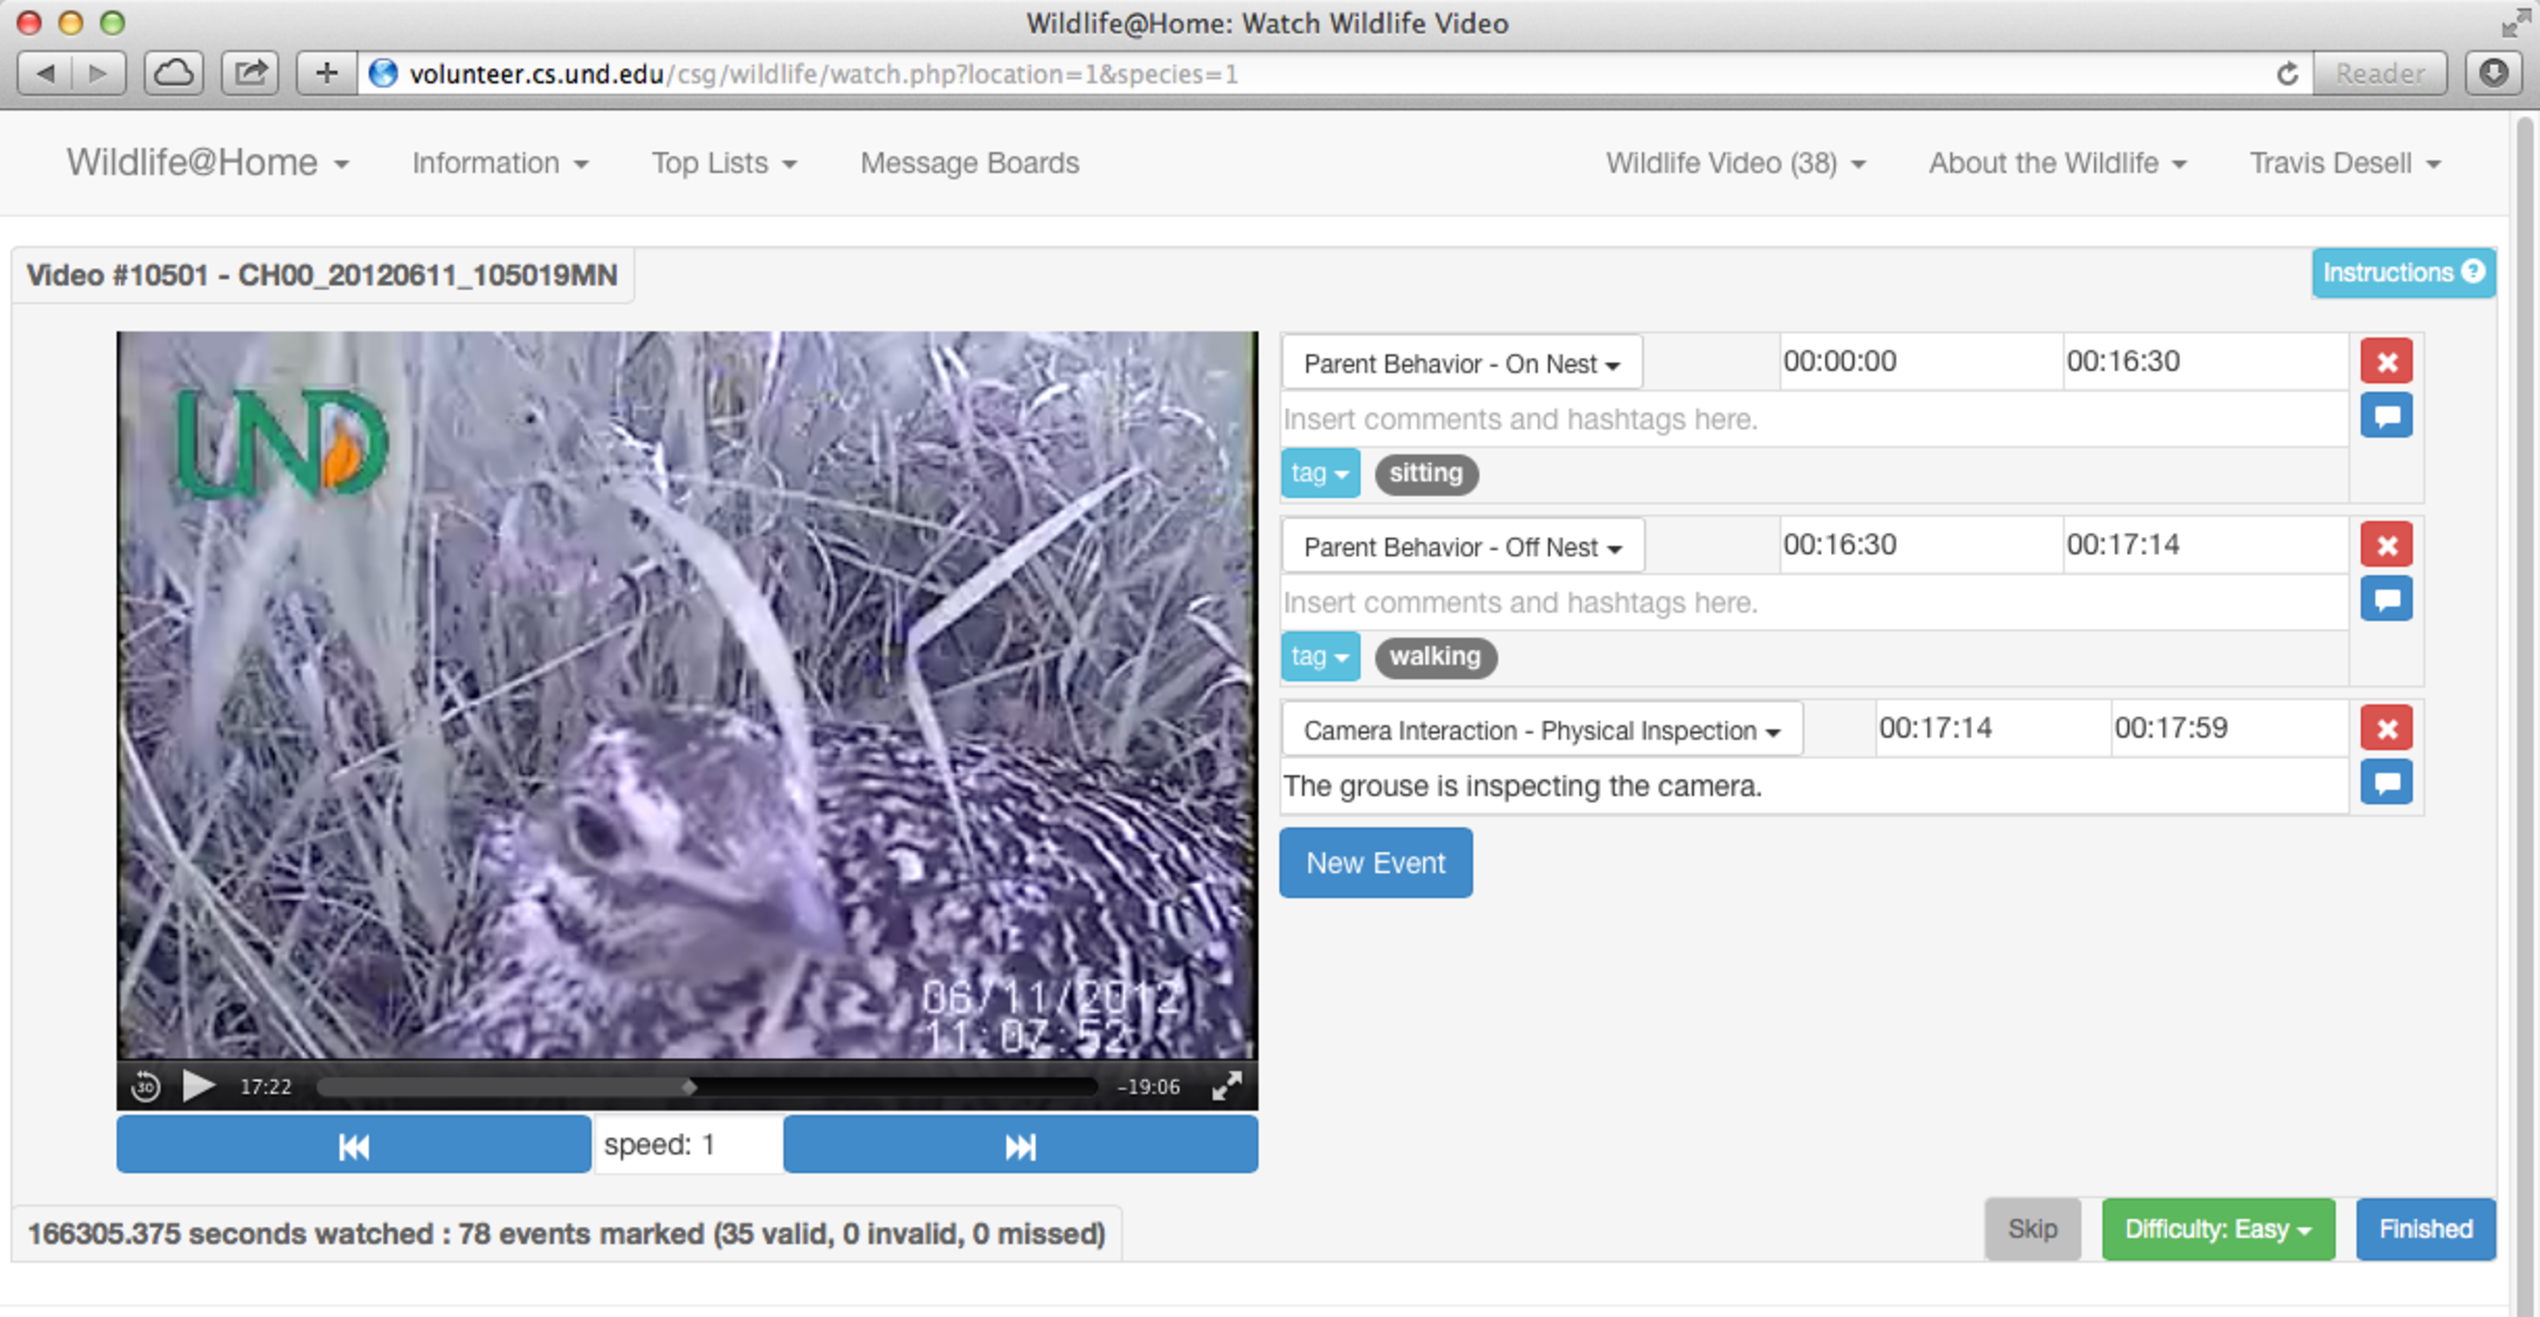
\includegraphics[width=5.8in]{./img/crowd_source_example_new.pdf}
\caption{An example of Wildlife@Home's video viewing interface. Users are shown 30 minute to 2 hour long nesting videos, and can specify the start and end time for various events of interest, and provide tags and comments for additional detail. Users can also specify how difficult it was to determine events for the video and discuss segments of the video on the project's message boards.}
\label{fig:wildlife_interface}
\end{figure*}

The Wildlife@Home project has accumulated over 85,000 hours of 24/7 uncontrolled outdoor surveillance video. This amount of data becomes problematic for humans to classify, even with software tools to help create and store event data. A lot of time is spent viewing regions of the video where the birds are not present at all or where a bird is present but highly inactive for long periods of time. Users watching video use the scrub bar to move more quickly through the video, especially uninteresting potions, and this can cause missed events. Scientists tasked with classifying long periods of uninteresting video can more quickly tire and lose focus.

This paper investigates the use of computer vision, machine learning, and background subtraction for the detection of avian nesting behaviors. The machine learning attempts to mimic the functionality of the human scientists by using image feature detection (SIFT~\cite{lowe_1999_object} \& SURF~\cite{bay_2006_surf}) and a support vector machine (SVM~\cite{burges_1998_tutorial, carpenter_2009_cusvm, chang_2007_psvm, chang_2011_libsvm}) to classify video frames. The background subtraction techniques focus on highlighting interesting or active section of video in order to aid scientists in behavior classification.

Feature detection and machine learning are effective for detection and classification of rigid objects~\cite{faro_2011_adaptive} but has also shown success in the recognition of pedestrians and some wildlife~\cite{heikkila_2004_real, dalal_2005_histograms, fan_2013_pedestrian,oren_1997_pedestrian, boom_2012_long}. We test the effectiveness of this method by using scientist observations as training data and compare algorithm performance in recognizing bird nesting behaviors.

Background subtraction is commonly used in surveillance video as a technique for segmenting objects of interest from a scene~\cite{mcivor_2000_background, piccardi_2004_background}. By extracting segments of the collected video with an abnormal amount of foreground activity, it is possible to algorithmically present scientists with video containing classifiable events and filter out video where no events occur.

While both methods focus on reducing scientist workload, they use very different methods to do so. The machine learning method attempts to determine an event type for each video frame by learning form previous classifications made by scientists. Each video frame is tagged with ongoing events and descriptors collected from that frame are used with a support vector machine to learn bird behaviors. The goal of this process is to automatically classify nesting behaviors, especially \emph{in video} and \emph{not in video} events. The background subtraction focuses on eliminating work for scientists by finding sections of video with bird activity or \emph{interesting} events. Background subtraction doesn't allow for classification of events but can greatly reduce scientist workload.

Feature detection with SURF and event classification with LIBSVM~\cite{chang_2011_libsvm} has shown to be a poor performer on the Wildlife@Home video. Many factors may cause poor performance on the footage, including video quality, brightness fluctuations, species cryptic coloration, and slightly incorrect event boundaries set by scientists. The poor results seen from this research sparked a shift to study the effectiveness of background subtraction in the same domain.

Given the diversity of species and nest locations, results find that background subtraction performance is sensitive to the amount of background movement, camera brightness, and cryptic coloration in a video. Using modern background subtraction techniques, such as Mixture of Gaussians (MOG)~\cite{power_2002_understanding}, and modified versions of the ViBe~\cite{van_2014_vibe} and Pixel-Based Adaptive Segmentation (PBAS)~\cite{hofmann_2012_background} algorithms, it is possible to show a strong correlation between scientist observed events and those calculated with background subtraction. By confidently narrowing the amount of video scientists are watching, it will be possible to focus on showing worth-while video segments and increase user incentive and focus.

Chapter~\ref{ch:related_work} presents modern techniques used for common feature detection algorithms, SVMs, and background subtraction problems. Chapter~\ref{ch:methodology} covers the approaches we took to classifying frames and extracting regions of the video with activity. Performance results and limitations of the algorithms are in described Chapter~\ref{ch:results}. Finally, Chapter~\ref{ch:conclusion} concludes with future work and a discussion of the next steps to collecting more results, improving the algorithms, and use of the data.

\begin{figure*}[!t]
\centering
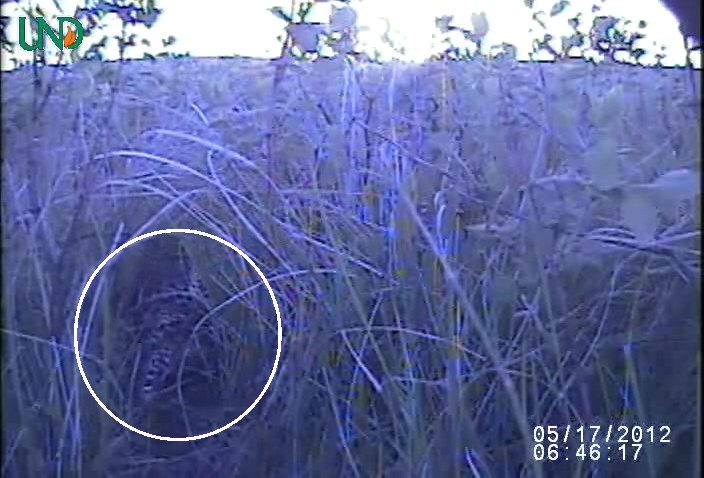
\includegraphics[width=2.5in]{6396_sample_grouse}
\caption{Sample Sharp-Tailed Grouse footage. The nest is marked with a white oval.}
\label{fig:sample_grouse}
\end{figure*}

\begin{sidewaysfigure}[!t]
\centering
\subfloat[Sample I]{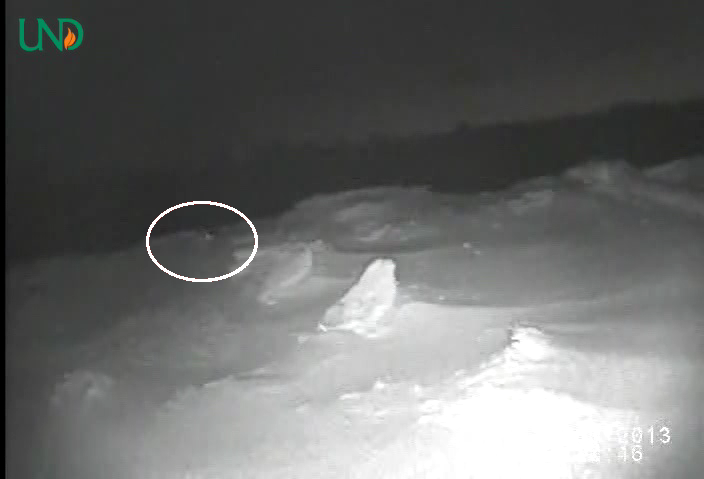
\includegraphics[width=2.9in]{59032_1}
\label{fig:first_case}}
\hfil
\subfloat[Sample II]{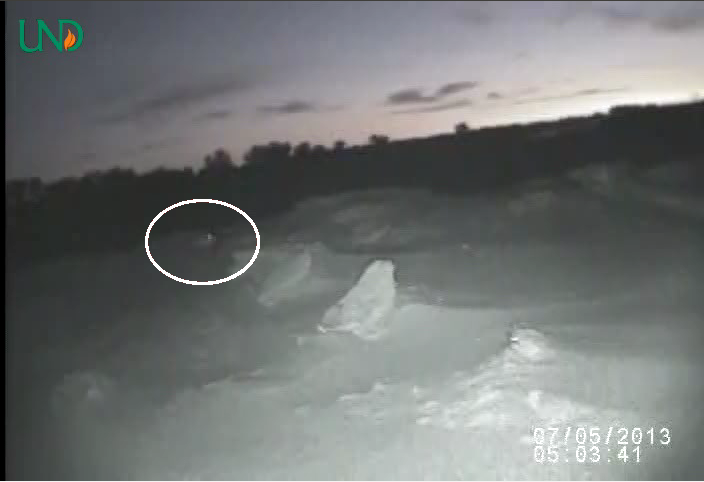
\includegraphics[width=2.9in]{59032_2}
\label{fig:second_case}}
\hfil
\subfloat[Sample III]{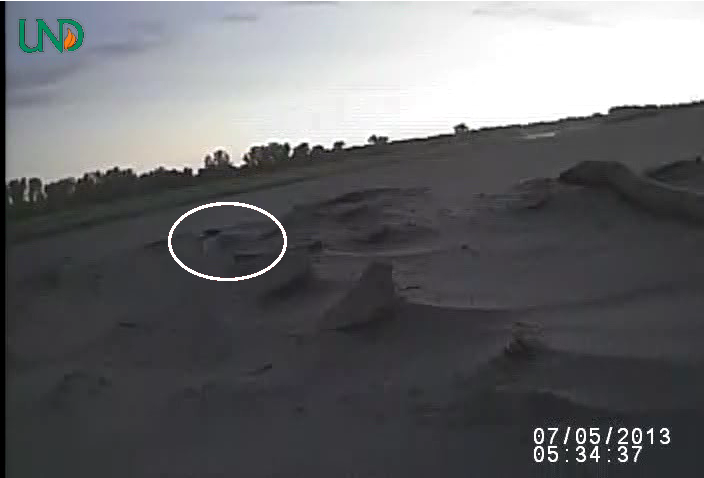
\includegraphics[width=2.9in]{59032_3}
\label{fig:third_case}}
\caption{Sample sunrise Interior Least Tern footage. The nest is marked with a white oval.}
\label{fig:example_tern_video}
\end{sidewaysfigure}


\chapter{Related Work} \label{ch:related_work}

%----------------------------------------
% AIRCRAFT OPERATIONS
%----------------------------------------
\section{Aircraft Operations}

	In Dr. Ed Wischmeyer's paper, \emph{The Myth of the Unstable Approach}~\cite{wischmeyer2004the-myth}, he discusses how the term ``unstable approach'' is now becoming too vague to be used in accident and incident reports.  He argues there are too many factors that play into an approach; therefore, labeling it solely as an ``unstable approach'' is not sufficient.  This aligns with one of the goals of the \toolname\ in that it was developed to detect unstable approaches and be able to state what the specific parameter was that caused the approach to be unstable.  In doing this, it allows for finer-grained statistics to be generated, which can reveal further patterns to be detected within an organization if it becomes a wide-spread problem.
    
    Nazeri \etal~\cite{Nazeri:2008:Analyzing-Relat} researched accident and incident data from several different commercial flight data sources in order to discover the factors that cause those events.  They created eight high-level categories, each with sub-factors, for classification.  They used an algorithm to analyze the data for correlations between different attribute-value pairs across the accident and incident data sets.  A factor support ratio was calculated for each attribute-value pair and ranked in decreasing order to find the most significant factors.  The following high-level factors were the four top ranked in order:  company, air traffic control, pilot, and aircraft.  They also did a time-series analysis of the data for the ten-year period in which the data was collected (1995-2004).  This time-series data showed the pilot and aircraft factors are generally decreasing over time, while the air traffic control factors are generally increasing.  By uncovering these patterns and analyzing them over time, they were able to find the factors that are leading causes for accidents/incidents and can address these factors for improvement.


%----------------------------------------
% POST-FLIGHT EVALUATION TOOLS
%----------------------------------------
\section{Post-Flight Evaluation Tools}

	There are several software projects that have created post-flight evaluation tools, which a pilot can use to analyze their performance during various phases of flight.  Each project has a similar methodology, but varying presentation techniques.  Knighton and Claramunt~\cite{knighton2001an-aeronautical} created a system that included hardware for collecting real-time flight data and an interactive graphical user interface (GUI).  The GUI is capable of 2D flight re-animation and simple plots of the aircraft's vertical profile throughout the flight.  The flight re-animation also has a panel with indicators showing the real-time sensor data at each time step.  They found through experiments using volunteers that their interface was intuitive and encouraged exploration of different aspects of flight performance.  Despite the usefulness of the flight parameter graphs, the downside to their research is that any analysis has to be performed manually by the user as there are no automated analysis results provided.
    
    Masiulionis and Stankunas~\cite{masiulionis2017review} provide a review of several software packages for flight analysis including \textit{IGC Flight Replay}, \textit{OziExplorer}, \textit{GPS TrackMaker}, and \textit{ArcGIS}.  They found that none of the packages provided all the aspects they sought:  interactively enabling/disabling map layers, graphing multiple flight parameters on a single plot, and high-resolution maps.  Thus, they experimented with flight analysis and visualization using \textit{Google Earth}.  \textit{Google Earth} met all of their standards, but the only disadvantage is that the altitude and speed graphs can become compressed for flights with an extended duration.  It does not include any features to resize or drill-down into the graphs to make them more viewable. \note{comment on how mine is different}
    
    Goblet \etal~\cite{goblet2016phase,goblet2015identifying} researched into automatically classifying phases of GA flights.  The focus is on the Climb, Cruise, and Descent phases as they are the most difficult phases to identify in GA due to the variation of mission profiles and purposes of flight when compared to Commercial Aviation. Several methods were explored for identifying these phases:  altitude-based and smoothing-and-differentiation-based (which includes down-sampling, moving average, and local regression).  It was found the best method to use for a particular flight is determined by specific characteristics found within that flight.  An algorithm is then given to automatically select the best method for each flight.  Although the Climb, Cruise, and Descent phases are the most difficult to identify, it is known that the Takeoff, Approach, Landing, and Go-Around phases are the most critical and dangerous in GA (as discussed in \Cref{ch:introduction}), thus is the reason this work focuses on analysis of those phases. 
    
    Fala and Marais~\cite{fala2016detecting} developed a method of detecting unsafe aircraft parameters, termed ``safety events'', in GA flights.  Similar to phase identification, detecting safety events in GA is difficult due to the variability in operations.  In their research, they only focus on the Approach phase and provide the numerical parameter limits for a Cirrus SR20 aircraft during the Approach phase.  For each parameter, they provide a Level 1 and Level 2 limit stating that Level 2 is more dangerous than Level 1.  They analyzed the Approach phases from a sample of 23 flights using their defined thresholds and performed a one-way ANOVA analysis to evaluate whether the average number of instances for each type of safety event was similar.  They found their initial threshold definitions were not similar enough across the parameters.  They revised the definitions, re-analyzed the flights, and performed another ANOVA analysis to find that they were then significantly similar.  When detecting safety events, Fala and Marais did not distinguish between sporadic exceedances of the thresholds and a span of consecutive exceedances.  This differs from the work in this project, where an event can span multiple seconds instead of only single time steps.\todo{explain why I chose this approach}
	

%----------------------------------------
% NGAFID RELATED WORK
%----------------------------------------
\section{NGAFID Related Work}

	Other work on the NGAFID has focused in two different areas.  In the first, Desell \etal\ have examined methods based on the prediction of flight data parameters using recurrent neural networks (RNNs).  They have shown that training Jordan and Elman RNNs using evolutionary algorithms such as Particle Swarm Optimization and Differential Evolution can provide strong predictive results for flight data parameters such as airspeed, altitude, pitch, and roll~\cite{desell2014evolving}; and that these results can be further refined utilizing a novel neuroevolution technique based on ant colony optimization to evolve the structure of the RNNs~\cite{desell2015evolving}. Further work by ElSaid \etal\ has utilized Long Short-Term Memory (LSTM) RNNs to predict aircraft engine vibration events~\cite{elsaid2016vibration,elsaid2016thesis}.
    
    The other area has been in utilizing unsupervised machine learning methods to detect anomalous flights.  Clachar \etal\ have used self organizing maps (SOMs), a type of neural network, to both cluster time series flight data and identify anomalous flights~\cite{sophine2014identifying,sophine2016phd} based on approach phases, with SOMs providing significant benefits in terms of parallelism and performance over other clustering methods such as DBSCAN.


%----------------------------------------
% DATA MINING TECHNIQUES
%----------------------------------------
\section{Data Mining Techniques}

	Harris \etal~\cite{harris-jr.1998recent} of MITRE Corporation mined accident and incident reports provided by the International Civil Aviation Organization (ICAO) in order to determine the specific attributes that were the cause in each kind of report and also needed to be considered ``interesting'' (i.e., anything that is an exception to commonly accepted knowledge among aviation experts) by the aviation expert who collaborated with them.  They discovered that using traditional data mining methods was not sufficient enough to find ``interesting'' results.  This is because experts have studied the field of aviation so extensively that all the obvious rules and correlations have already been discovered.  Next, they developed their own system called Smithers, which uses a technique called attribute focusing, that finally uncovered an interesting correlation which shows that having an advanced heads up display (HUD) can help reduce the amount of damage as a result of a runway incursion\footnote{Defined by the Federal Aviation Administration (FAA) as, ``any occurrence at an aerodome involving the incorrect presence of an aircraft, vehicle, or person on the protected area of a surface designated for the landing and take off of aircraft''~\cite{federal-aviation-administrationrunway}.}.  This shows that even though aviation safety has been studied extensively, there are still new correlations that can be made when applying several different data mining methods.
    
    Matthews \etal~\cite{matthews2013discovering} performed similar research in which their goal was to find anomalous data in flights.  They differ in the fact that they used algorithms that could analyze at both a fleet-level and flight-level.  Doing this allowed them to find anomalies for an entire organization or just a single flight, which makes it very useful in order to find patterns of problems.  This idea is similar to the NGAFID project in which flight data can be analyzed on multiple levels while giving statistics for each.

% !TEX root =  ../main.tex

\chapter{Methodology} \label{ch:methodology}

	The \toolname\ provides several features: \textit{(i)} phase of flight identification, \textit{(ii)} quality analysis of each phase, \textit{(iii)} grade assignment, and \textit{(iv)} a web interface to display results.  Since there are three separate phases of concern, there will be a separate subsection for each in both identification and quality analysis.  These features are discussed in more detail in the rest of this Chapter.

%----------------------------------------
% PHASE IDENTIFICATION
%----------------------------------------
\section{Phase of Flight Identification} \label{sec:phase_identification}

	%----------
    % APPROACH
    %----------
	\subsection{Approach}
    
    	The approach phase is defined as the time between the aircraft entering the airport's traffic pattern (shown in \Cref{fig:traffic_pattern}), or 1,000 feet above the runway elevation, to the beginning of the landing flare under Visual Flight Rules (VFR).  For Instrument Flight Rules (IFR), it is the time from the Initial Approach Fix (IAF) to the beginning of the landing flare~\cite{cictt2013phase}.
        
        \begin{figure}
        	\centering
            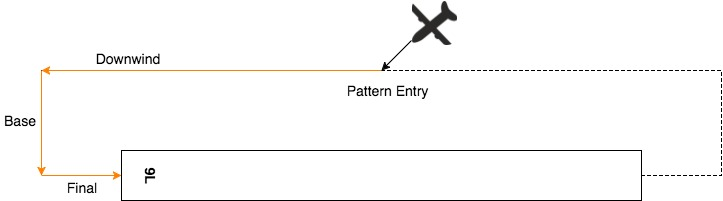
\includegraphics[width=\linewidth]{img/airport_traffic_pattern}
            \caption{Example showing an airport's traffic pattern and the subphases of the approach.}
            \label{fig:traffic_pattern}
        \end{figure}
        
        Along with detecting the approach phase (\Cref{alg:detect_approach}), this section also details the algorithms for detecting \textit{(i)} the airport and runway that the aircraft is approaching and \textit{(ii)} the final turn so it can later be analyzed for an undershoot or overshoot.
        
        The algorithm for detecting an aircraft's approach needs to iterate through all of the time values since there can be multiple approaches within a single flight.  Once the algorithm detects the aircraft is 1 mile away from an airport and is less than 500 feet above ground level (AGL) (\Cref{alg:detect_approach} Line 6), it is determined that the pilot is beginning an approach and a unique approach identifier is generated in order to store metadata later in the process.  Next, the algorithm continues to iterate through time values until either the aircraft goes under 200 ft AGL, or it goes back above 500 ft AGL, which will then be recorded as a go-around later in the process (\Cref{alg:detect_approach} Lines 8-12).  If the aircraft goes under 200 ft AGL, then it is determined to be on the final approach.  The aircraft is considered to be on the final approach while it is within 1 mile away from the airport and it is between 50 and 200 feet AGL inclusive (\Cref{alg:detect_approach} Lines 16-22).
    
    Once the aircraft either goes above 200 feet AGL or goes below 50 feet AGL, then the final approach is marked as finished, and the critical metadata associated with the approach is stored.  At this point, the runway that is being approached can be detected using a combination of the aircraft's current geolocation and heading since the intended runway may not be closest to the aircraft depending on the degree of the final turn (\Cref{alg:detect_approach} Line 24).
        
        %%%%% Detect Approaches Pseudo-code
        \begin{algorithm}
            \begin{algorithmic}[1]\raggedright
            	\State $ \var{airplanePoint} \gets \var{data[i].geoPoint} $
            	\State $ \var{airport} \gets \var{detectAirport(airplanePoint)} $
                \State $ \var{airplaneAltitude} \gets \var{data[i].altitude} $
                \State $ \var{heightAGL} \gets \var{airplaneAltitude} - \var{airport.altitude} $
                \State $ \var{distance} \gets \var{airplanePoint.distanceTo(airport.geoPoint)} $
                \If{$ \var{distance} < 1$\,mi and $\var{heightAGL} < 500$\,ft}
                    \State $ \var{apprID} \gets \var{genNewApproachID()} $
                    \While{$ 200\,\text{ft} < \var{heightAGL} < 500\,\text{ft} $ and $ \var{i} < \var{data.length} $}
                        \State $ \var{airplaneAltitude} \gets \var{data[i].altitude} $
                        \State \var{heightAGL} $ \gets $ \var{airplaneAltitude} $-$ \var{airport.altitude}
                        \State $ i \gets i + 1 $
                    \EndWhile

                    \State $ \var{approachStartTime} \gets i $
                    \State $ \var{airplaneHdg} \gets \var{data[i].hdg} $
                    \State $ \var{airplanePoint} \gets \var{data[i].geoPoint} $

                    \While{$ \var{distance} < 1$\,mi and $ 50\,\text{ft} \leq \var{heightAGL} \leq 200\,\text{ft} $ and $ \var{i} < \var{data.length} $}
                        \State $ \var{airplaneAltitude} \gets \var{data[i].altitude} $
                        \State $ \var{airplanePoint} \gets \var{data[i].geoPoint} $
                        \State $ \var{distance} \gets \var{airplanePoint.distanceTo(airport.geoPoint)} $
                        \State $ \var{heightAGL} \gets \var{airplaneAltitude} - \var{airport.altitude} $
                        \State $ i \gets i + 1 $
                    \EndWhile

                    \State $ \var{approachEndTime} \gets i $
                    \State $ \var{runway} \gets $ \var{detectRunway(airplanePoint, airplaneHdg, airport)}
                    \State \var{approaches[apprID]} $ \gets $ store approach metadata
                    \State \Return \var{(approachStartTime, approachEndTime)}
                \EndIf
            \end{algorithmic}
            \caption{Pseudo-code for function which detects when an aircraft is approaching a runway.}
            \label{alg:detect_approach}
        \end{algorithm}
        
        
        %----------
        % AIRPORT DETECTION
        %----------
        \subsubsection{Airport detection.} \label{sec:detect_airport}
        
        	For identifying the airport that is being approached, a QuadTree~\cite{finkel1974quad} data structure was used.  It was used due to the fact that a two-dimensional tree structure is needed in order to efficiently find the closest airport latitude and longitude point when given the aircraft's latitude and longitude.  The QuadTree is constructed using a list of airport objects from a database then is optimized.  Both the insertion and searching algorithms yield $\mathcal{O}(\log n)$ complexity.


        %----------
        % RUNWAY DETECTION
        %----------
        \subsubsection{Runway detection.}
        
            The algorithm used for finding the runway that is being approached is a simple sequential search with a constraint that the difference between the aircraft's heading and the runway's heading must be within an upper limit.  The reasoning for this constraint is the fact that the runway closest to the aircraft may not necessarily be the one it is approaching depending on the arrangement of the runways and the degree of the final turn (see \Cref{fig:runway_selection}).  A value of $20^\circ$ was used for the heading constraint since it is double the value used for detecting a heading exceedance (see \Cref{tab:approach_thresholds}).  Thus if the runway returned by the algorithm is not the intended runway, it means the aircraft's heading is significantly off-center from the runway's heading and the pilot will need to perform severe corrections to get back on course.
            
            In this case, using a sequential search is efficient enough since an airport has a very small number of runways, whereas there are thousands of airports within the United States which requires a more sophisticated algorithm.  The runway detection algorithm is given in \Cref{alg:detect_runway}.
            
            
            \begin{figure}
            	\centering
				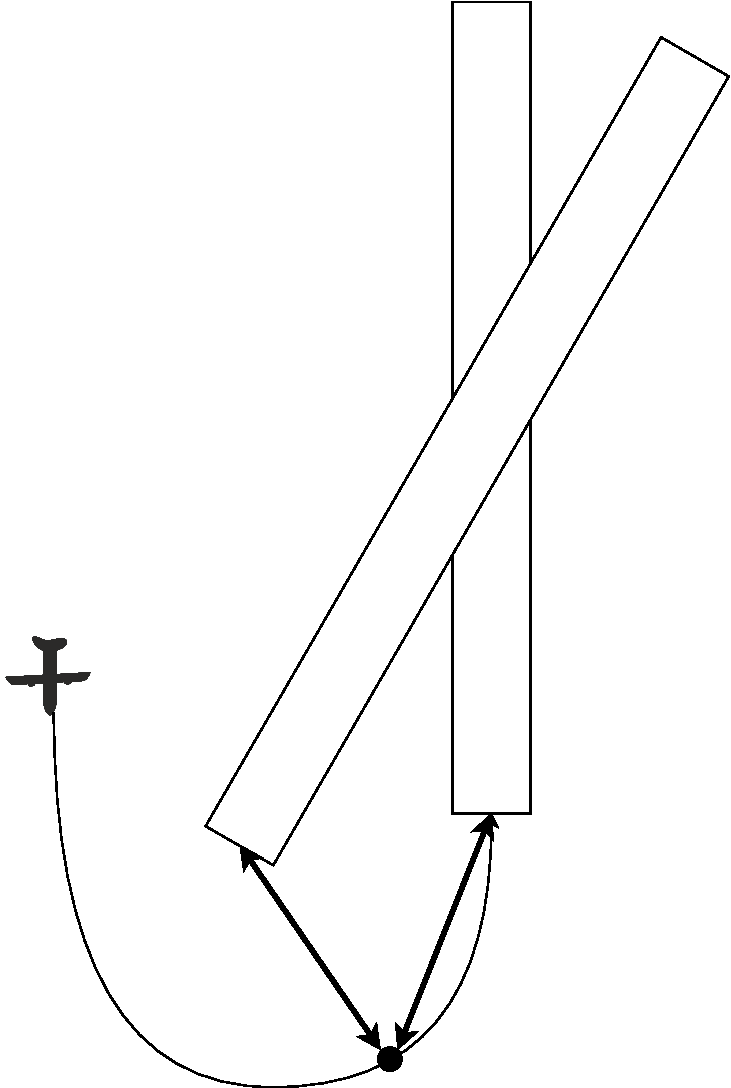
\includegraphics[width=0.5\linewidth]{runway_selection_example}
				\caption{Example showing that the closest runway to the aircraft may not necessarily be the one they are attempting to land on.  If we use the black dot as a reference point for when we attempt to detect the runway, it can be seen that the runway on the left may actually be closer.  However, the aircraft's heading will match closer to the runway on the right (the pilot's intended target).  This is the purpose of searching for the closest runway with a constraint on the heading difference.}
				\label{fig:runway_selection}
            \end{figure}
            

            %%%%% Detect Runway Pseudo-code
            \begin{algorithm}
                \begin{algorithmic}[1]\raggedright
                    \Function{DetectRunway}{airplanePoint, airplaneHdg, airport}
                        \State $ \var{theRunway} \gets \textit{NULL} $
                        \State $ \var{closestDistance} \gets \infty $

                        \For{\var{runway} in \var{airport.runways}}
                            \If{$ \abs{\var{headingDifference(runway.hdg, airplaneHdg)}} \leq 20^\circ $}
                                \State $ \var{distance} \gets \var{airplanePoint.distanceTo(runway.geoPoint)} $
                                \If{$ \var{distance} \le \var{closestDistance} $}
                                    \State $ \var{theRunway} \gets \var{runway} $
                                    \State $ \var{closestDifference} \gets \var{difference} $
                                \EndIf
                            \EndIf
                        \EndFor

                        \State \Return{theRunway}
                    \EndFunction
                \end{algorithmic}
                \caption{Pseudo-code for \textit{detectRunway} function which detects the runway an aircraft is approaching.}
                \label{alg:detect_runway}
            \end{algorithm}
        
        
        %----------
        % FINAL TURN DETECTION
        %----------
        \subsubsection{Final turn detection.}
        
        	In order to detect the final turn subphase of the approach, we first get the previous three minutes of data before the approach ends.  The previous three minutes are used to reduce the search space and because it does not make logical sense for a final turn to occur greater than three minutes before the approach ends.  Next, the algorithm searches for the final turn start and end time.  It finds these by searching for the points at which the aircraft's heading creates a $90^\circ$ and $15^\circ$ angle, respectively, to the runway's heading.  A visualization of these reference points can be seen in \Cref{fig:final_turn_example}.  The search is performed backwards through the slice of data in order to obtain the last occurrence of each angle difference.  Once both points have been found, they are stored for later use in the analysis stage.  If the aircraft did not have a heading difference greater than $90^\circ$ in the final three minutes, the pilot performed a straight-in approach and, consequently, did not execute the final turn subphase.
        	The final turn detection algorithm is given in \Cref{fig:detect_final_turn}.
            
            \begin{figure}
            	\centering
                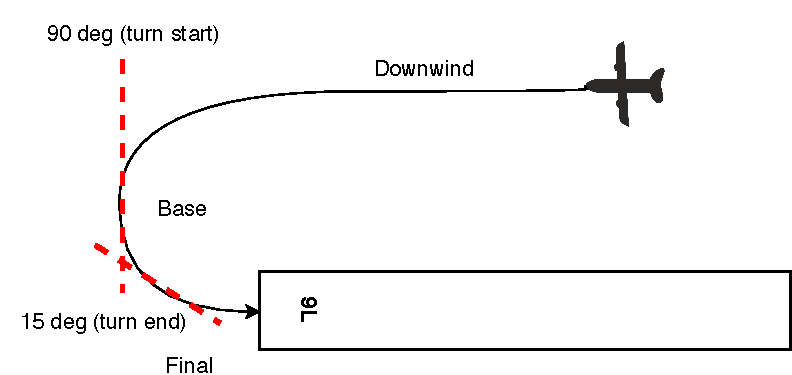
\includegraphics[width=\linewidth]{turn_to_final}
                \caption{Example showing the approach subphases and the slice of data used in the final turn analysis.  The dashed lines represent when the final turn starts ($90^\circ$ heading difference) and ends ($15^\circ$ heading difference).}
                \label{fig:final_turn_example}
            \end{figure}
        
            %%%%% Detect Final Turn Pseudo-code
            \begin{algorithm}
                \begin{algorithmic}[1]\raggedright
                    \Function{DetectFinalTurn}{approachEndTime, runway}
                        \State $ \var{last3Mins} \gets $ get previous 3 mins of data before \var{approachEndTime}
                        \State $ \var{turnStartTime} \gets \textit{NULL} $
                        \State $ \var{turnStartFound} \gets \textit{false} $
                        \State $ \var{turnEndTime} \gets \textit{NULL} $
                        \State $ \var{turnEndFound} \gets \textit{false} $
                        \State $ \var{i} \gets \var{last3Mins.length} - 1 $
                        
                        \Comment Loop backwards through the last 3 mins of data
                        \While{not \var{turnStartFound} and not \var{turnEndFound} and $\var{i} \geq 0$}
                        	\State $ \var{headingError} \gets \abs{\var{headingDifference(runway.hdg, last3Mins[i].hdg)}} $
                            \If{$\var{headingError} \geq 90$ and not \var{turnStartFound}}
                            	\State $ \var{turnStartTime} \gets \var{i} $
                                \State $ \var{turnStartFound} \gets \textit{true} $
                            \EndIf
                            \If{$\var{headingError} \geq 15$ and not \var{turnEndFound}}
                            	\State $ \var{turnEndTime} \gets \var{i} $
                                \State $ \var{turnEndFound} \gets \textit{true} $
                            \EndIf
                            
                            \State $ \var{i} \gets \var{i} - 1 $
                        \EndWhile
                        
                        \State $ \var{approaches[apprID]} \gets $ store final turn metadata
                        \State \Return \var{(turnStartTime, turnEndTime)}
                    \EndFunction
                \end{algorithmic}
                \caption{Pseudo-code for function which detects the final turn subphase of the approach.}
                \label{fig:detect_final_turn}
            \end{algorithm}
        
        
    
    %----------
    % LANDING
    %----------
    \subsection{Landing}
    
    The landing phase is defined as the time from the beginning of the landing flare until the aircraft performs one of the following actions: \textit{(i)} exits the landing runway, \textit{(ii)} comes to a complete stop on the runway (full-stop), or \textit{(iii)} when power is applied for takeoff in the case of a touch-and-go landing~\cite{cictt2013phase}.
    
    The landing phase and result detection is able to differentiate between a full-stop, touch-and-go, and a go-around\footnote{Go-around is included here as a possibility for the result of a landing phase since only one of the full-stop, touch-and-go, and go-around maneuvers can be executed after an approach/landing even though the aircraft does not physically contact the ground.}.  Pseudo-code for this process is given in \Cref{alg:detect_landing}.
    
    This detection algorithm iterates through time values starting where the final approach detection finished (\Cref{alg:detect_landing} Lines 10-29).  It continues to iterate while the aircraft is below 500 feet AGL; or if it is the aircraft's final landing and the time values run out, then it stops analyzing.  While the algorithm iterates through the time values, it checks if the aircraft's indicated airspeed (IAS) is less than or equal to 35 knots (\Cref{alg:detect_landing} Line 13).  If this is true, then it is determined the aircraft is no longer traveling at a flying speed, thus it is making a complete stop.  The stall speed of a Cessna 172S aircraft is 40 knots IAS (KIAS)~\cite{und_poh}; therefore, the value of 35 knots guarantees the aircraft cannot be flying.  In order to detect a touch-and-go landing, the previous five elevation readings are stored and their average is calculated (\Cref{alg:detect_landing} Lines 20-28).  If it is found the aircraft is not making a stop-and-go landing, then the average elevation for the last five seconds is checked to see if it is less than five feet AGL (\Cref{alg:detect_landing} Line 15).  This means the aircraft is still at a flying speed (above 35 knots) and is also maintaining a stable elevation of five feet or less for at least five seconds.
    
    Once the aircraft goes above 500 feet AGL or the time values run out, then the landing result is determined from the conditions found during the analysis (\Cref{alg:detect_landing} Line 32 and \Cref{alg:landing_result_helper}).  If it was found the aircraft was making a complete stop, then a value of ``full-stop'' is stored.  If it was not making a complete stop and had a relatively stable elevation of 5 feet or less above the runway, then a value of ``touch-and-go'' is stored.  The final result type, ``go-around'', is used as a fall-through since there are only three classifications, as mentioned previously.  The three landing result types and how they are detected are summarized in \Cref{tab:landing_types}.
    
    After the landing is classified, then it is determined whether there is a takeoff phase that follows the current landing phase.  If the end of the data has been reached or a go-around is being performed (\Cref{alg:detect_landing} Line 33), there will not be a subsequent takeoff phase.  Otherwise, we need to find the transition from landing to takeoff.  This is done by finding the index of the engine's minimum RPM value between \textit{landingStartTime} and \textit{landingEndTime} (\Cref{alg:detect_landing} Line 36 and \Cref{alg:last_rpm_helper}).  By using the engine's minimum RPM value, we know all RPM values afterwards will be greater, which means the pilot will be using more throttle in order to takeoff.  The \textit{landingEndTime} is then reset to this transition mark.  Lastly, the critical metadata found during the analysis is stored.
    
    %%%%% Detect Landing Pseudo-code
   	\begin{algorithm}
    	\begin{algorithmic}[1]
        \Function{DetectLanding}{approachEndTime, runway}
        	\State $ \var{landingStartTime} \gets \var{approachEndTime} $
        	\State $ \var{i} \gets \var{approachEndTime} $
        	\State $ \var{airplaneAltitude} \gets \var{data[i].altitude} $
            \State $ \var{heightAGL} \gets \var{airplaneAltitude} - \var{runway.altitude} $
            
            \State $ \var{isFullStop} \gets \textit{false} $
            \State $ \var{isTouchAndGo} \gets \textit{false} $
            \State $ \var{elevations} \gets \var{[]}$
            \State $ \var{avg5SecElevation} \gets 5\,\text{ft} + 1 $
            	\Comment value to guarantee first check passes
            
            \While{$\var{heightAGL} < 500$\,ft and $\var{i} < \var{data.length}$}
            	\If{not \var{isFullStop}}
                	\State $ \var{airplaneIAS} \gets \var{data[i].ias} $
                    \If{$ \var{airplaneIAS} \leq 35$\,kts}
                    	\State $ \var{isFullStop} \gets \textit{true} $
                    \ElsIf{$ \var{avg5SecElevation} \leq 5$\,ft}
                    	\State $ \var{isTouchAndGo} \gets \textit{true} $
                    \EndIf
                \EndIf
                \State $ i \gets i + 1 $
                \State $ \var{airplaneAltitude} \gets \var{data[i].altitude} $
                \State $ \var{heightAGL} \gets \var{airplaneAltitude} - \var{runway.altitude} $
                \If{$ \var{elevations.length} < 5$\,seconds}
                	\State $ \var{elevations.append(heightAGL)} $
                \Else
                	\State $ \var{elevations.pop()} $
                    \State $ \var{elevations.append(heightAGL)} $
                    \State $ \var{avg5SecElevation} \gets \var{avg(elevations)} $
                \EndIf
            \EndWhile
            
            \State $ \var{landingEndTime} \gets \var{i} $
            \State $ \var{isEndOfData} \gets \var{landingEndTime} == \var{data.length} - 1 $
            
            \State $ \var{landingResult} \gets \var{getLandingResult(isFullStop, isTouchAndGo)} $
         
            \State $ \var{isFollowedByTakeoff} \gets not (\var{isEndOfData} $ or $ \var{landingType} == \text{`go-around'}) $
            
            \Comment{If landing is followed by a takeoff, then we need to find the transition from landing to takeoff}
            \If{\var{isFollowedByTakeoff}}
            	\State $ \var{landingDataSlice} \gets $ get slice of data between \var{landingStartTime} and \var{landingEndTime}
                
                \Comment{Marks where the pilot is transitioning from landing to takeoff}
            	\State $ \var{lastOccurrence} \gets \var{getLastOccurrenceOfMinRPM(landingDataSlice)} $
                \State $ \var{landingEndTime} \gets \var{lastOccurrence} $
            \EndIf
            
            \State $ \var{approaches[apprID]} \gets $ store landing metadata
            \State \Return \var{(landingStartTime, landingEndTime)}
        \EndFunction
        \end{algorithmic}
        \caption{Pseudo-code for function which detects the landing from its associated approach.}
        \label{alg:detect_landing}
    \end{algorithm}
    
    
    \begin{algorithm}
    	\begin{algorithmic}[1]
        	\Function{GetLandingResult}{isFullStop, isTouchAndGo}
        		\If{\var{isFullStop}}
                    \State $ \var{landingResult} \gets $ `full-stop'
                \ElsIf{\var{isTouchAndGo}}
                    \State $ \var{landingResult} \gets $ `touch-and-go'
                \Else
                    \State $ \var{landingResult} \gets $ `go-around'
                \EndIf
                \State \Return \var{landingResult}
            \EndFunction
        \end{algorithmic}
        \caption{Pseudo-code for \var{getLandingResult} helper function.}
        \label{alg:landing_result_helper}
    \end{algorithm}
    
    
    \begin{algorithm}
    	\begin{algorithmic}[1]
        	\Function{GetLastOccurrenceOfMinRPM}{dataSlice}
        		\State $ \var{minRPM} \gets \var{min(dataSlice[`rpm'])} $
                \State $ \var{lastOccurrence} \gets 0 $
                \State $ \var{i} \gets 0 $
                
                \While{$\var{i} < \var{dataSlice.length}$} \Comment{loop through slice of data to find last occurrence of minimum RPM}
                	\If{\var{dataSlice[i].rpm} == \var{minRPM}}
						\State $ \var{lastOccurrence} \gets \var{i} $
                    \EndIf
                \EndWhile
                \State \Return \var{lastOccurrence}
            \EndFunction
        \end{algorithmic}
        \caption{Pseudo-code for \var{getLastOccurrenceOfMinRPM} helper function.}
        \label{alg:last_rpm_helper}
    \end{algorithm}
    
    %%%%% Landing Types Table
    \begin{table}
        \caption{\small{Landing result types and their conditions.}}
        \label{tab:landing_types}
        \vspace{3pt}
        \centering
        \begin{tabular}{@{} c m{.70\linewidth} @{}}
            \hline
            \bfseries Type & \bfseries Condition \\ \hline
            full-stop    & Aircraft's indicated airspeed speed (IAS) falls below 35 knots \\ \hline
            touch-and-go & Aircraft is not making a complete stop and maintains a stable altitude of five feet AGL or less for at least five seconds \\ \hline
            go-around    & All other cases \\ \hline
        \end{tabular}
    \end{table}
    

%----------------------------------------
% PHASE QUALITY ANALYSIS
%----------------------------------------
\section{Phase of Flight Quality Analysis \& Exceedance Detection} \label{sec:phase_quality}
    
    %----------
    % APPROACH
    %----------
	\subsection{Approach}
        
        Along with analyzing the approach phase, this section also details the algorithms for analyzing \textit{(i)} the final turn subphase for an undershoot or overshoot and \textit{(ii)} the pilot's self-defined glide path angle.
        
        The algorithm for analyzing an approach phase iterates through all the time values found during the phase identification stage (\Cref{alg:analyze_approach} Lines 4-17).  For each time value, the analysis for unstableness is performed.  During this analysis, several flight parameters are checked against predetermined thresholds to see if any were exceeded (\Cref{alg:analyze_approach} Lines 8-11).  The values used for the thresholds are summarized in \Cref{tab:approach_thresholds}.  A \textit{true} value for a condition means the parameter is stable.  Thus, if any of the parameters are unstable, \var{isUnstable} will result to being \textit{true}, meaning the entire aircraft is in an unstable state (\Cref{alg:analyze_approach} Line 12).  If the aircraft is found to be unstable, the corresponding time value is stored as well as the parameter values that caused the unstableness (\Cref{alg:analyze_approach} Line 14).
        
        %%%%% Exceedance Thresholds Table
        \begin{table}
            \caption{\small{Stabilized approach criteria for Cessna 172S~\cite{und_flight_manual}.}} \label{tab:approach_thresholds}
            \vspace{3pt}
            \centering
            \begin{tabular}{@{} c >{\raggedright\arraybackslash} m{.3\linewidth} m{.42\linewidth} @{}}
                \hline\noalign{\smallskip}
                \bfseries Parameter & \bfseries Description & \bfseries Value \\
                \noalign{\smallskip}
                \hline
                \noalign{\smallskip}
                F & Flight path correct & Less than 10$^\circ$ off runway heading, less than 50 ft left or right of the runway center line (cross track error) \\ \hline
                L & Landing configuration correct & N.A. \\ \hline
                A & Airspeed proper & Indicated airspeed (IAS) within 55-75 kts \\ \hline
                P & Power setting appropriate & N.A. \\ \hline
                S & Sink rate appropriate & Vertical speed indicated (VSI) does not exceed -1000 ft/min \\ \hline
            \end{tabular}
        \end{table}
        
        
        %%%%% Analyze Approach Pseudo-code
        \begin{algorithm}
            \begin{algorithmic}[1]\raggedright
            \Function{AnalyzeApproach}{startTime, endTime, runway}
                \State $ \var{approachDataSlice} \gets $ get slice of data between \var{startTime} and \var{endTime}
                \State $ \var{i} \gets 0 $
                \While{$\var{i} < \var{approachDataSlice.length}$}
                    \State $ \var{airplaneHdg} \gets \var{approachDataSlice[i].hdg} $
                    \State $ \var{airplaneIAS} \gets \var{approachDataSlice[i].ias} $
                    \State $ \var{airplaneVSI} \gets \var{approachDataSlice[i].vsi} $
                    \State $ \var{airplanePoint} \gets \var{approachDataSlice[i].geoPoint} $

                    \State $ \var{headingIsStable} \gets 180^\circ - \abs{\abs{\var{runway.hdg} - airplaneHdg} - 180^\circ} \leq 20^\circ $
                    \State $ \var{crossTrackIsStable} \gets \var{calculateCrossTrack(} \break \var{airplanePoint, airplaneHdg, runway)} \leq 50\,\text{ft} $
                    \State $ \var{iasIsStable} \gets 55\,\text{kts} \leq \var{airplaneIAS} \leq 75\,\text{kts} $
                    \State $ \var{vsiIsStable} \gets \var{airplaneVSI} \geq -1000\,\text{ft/min} $
                    \State $ \var{isUnstable} \gets $ not (\var{headingIsStable} and \var{crossTrackIsStable} and \var{iasIsStable} and \var{vsiIsStable})

                    \If{\var{isUnstable}}
                        \State $ \var{approaches[apprID]} \gets $ store index as unstable and corresponding unstable parameter values
                    \EndIf

                    \State $ \var{i} \gets \var{i} + 1 $
                \EndWhile
            \EndFunction
            \end{algorithmic}
            \caption{Pseudo-code for function which analyzes an approach for unstableness.}
            \label{alg:analyze_approach}
        \end{algorithm}
        
        
        %----------
        % Final Turn
        %----------
        \subsubsection{Final turn.}
        
        	The final turn subphase is very critical for achieving a flight path aligned with the runway.  Since the end of the turn occurs fairly late in the approach phase, any mistakes can greatly reduce the pilot's ability to stabilize the aircraft by 200 ft AGL.  If the pilot makes a turn that is too sharp (undershoot) or too wide (overshoot), they may have to make a large corrective maneuver to re-align themselves, which could stall the aircraft if performed incorrectly and potentially result in a loss of control (LOC) event.  Stalls and loss of control events contributed to 52.0\% and 17.4\% of all landing accidents in 2014~\cite{kenny201726th}, respectively. 
            
            Analyzing this subphase only requires the end time value and runway found during the identification stage.  For this single time value, the aircraft's cross track error is calculated (\Cref{alg:analyze_final_turn} Line 5).  Next, the direction of the turn is determined by calculating which roll attitude direction was greater\footnote{If the aircraft rolls to the left, it is recorded as a negative degree and vice versa if the aircraft rolls to the right.  This is why we find the minimum roll attitude as the highest degree in which aircraft rolled left, and the maximum roll attitude as the highest degree in which the aircraft rolled right.} (\Cref{alg:analyze_final_turn} Lines 6-12).  The severity of the cross track error is then determined (\Cref{alg:analyze_final_turn} Lines 13-19).  A Risk Level 1 error is a value greater than 25 feet, while a Risk Level 2 error is a value greater than 100 feet.  The turn error is determined next based on the roll direction and direction of the cross track error (\Cref{alg:analyze_final_turn} Lines 20-32).  For example, if the pilot rolled left and had a negative cross track error\footnote{Meaning they are left of the runway's centerline.}, it is considered an ``undershoot''.  See \Cref{tab:final_turn_matrix} for all possible combinations of roll direction and cross track error.  However, if the cross track error is less than a Level 1 risk, then the turn is considered to be safe and a Risk Level 0 is stored (\Cref{alg:analyze_final_turn} Line 18).  Lastly, the turn error and severity are stored.  See \Cref{fig:final_turn_examples} for visualizations of several different final turn scenarios.
            
            If a final turn was not found in the detection phase (due to the pilot performing a straight-in approach), the analysis stage will be skipped.
            
            
            \begin{figure}
            	\centering
                \subfloat[Aligned.\label{fig:aligned_example}]{
                	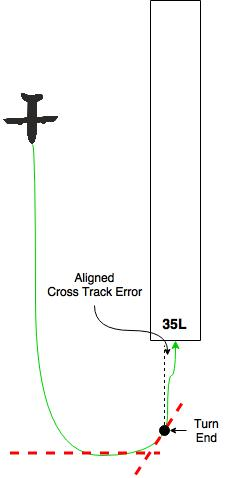
\includegraphics[width=0.29\textwidth]{img/aligned}
                }\hfill%
                \subfloat[Undershoot.  In this case, it is a small severity (Level 1) and color-coded as orange.\label{fig:undershoot_example}]{
                	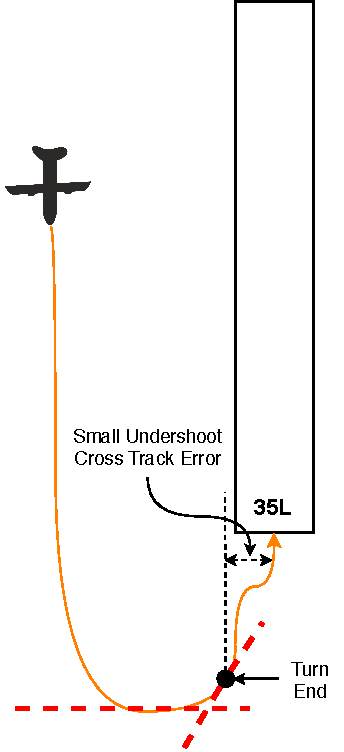
\includegraphics[width=0.29\textwidth]{img/undershoot}
                }\hfill%
                \subfloat[Overshoot.  In this case, it is a large severity (Level 2) and color-coded as red.\label{fig:overshoot_example}]{
                	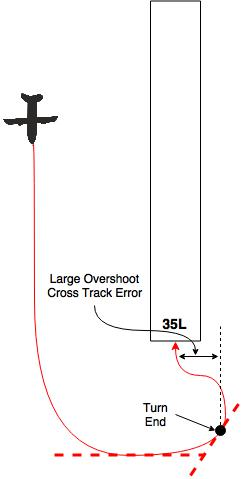
\includegraphics[width=0.29\textwidth]{img/overshoot}
                }%
                \caption{Examples showing various final turn qualities.}
                \label{fig:final_turn_examples}
            \end{figure}
            
            
            \begin{table}
            	\centering
                \caption{\small{Final turn matrix of the combinations of roll direction and cross track error.}} \label{tab:final_turn_matrix}
                \vspace{3pt}
                \begin{tabular}{|>{\bfseries}c | c c|}
                	\hline
                    \bfseries \diagbox{Direction}{Cross Track} & \bfseries $\mathbf{< 0}$\,ft & \bfseries $\mathbf{> 0}$\,ft \\
                    \hline
                    Left  & Undershoot & Overshoot \\ \hline
                    Right & Overshoot  & Undershoot \\ \hline
                \end{tabular}
            \end{table}
            
            
            %%%%% Analyze Final Turn Pseudo-code
            \begin{algorithm}
                \begin{algorithmic}[1]\raggedright
                \Function{AnalyzeFinalTurn}{startTime, endTime, runway}
                    \State $ \var{turnDataSlice} \gets $ get slice of data between \var{startTime} and \var{endTime}
                    \State $ \var{airplaneHdg} \gets \var{turnDataSlice[endTime].hdg} $
                    \State $ \var{airplanePoint} \gets \var{turnDataSlice[endTime].geoPoint} $
                    \State $ \var{crossTrackError} \gets \var{calculateCrossTrack(} \break \var{airplanePoint, airplaneHdg, runway)} $
                    
                    \State $ \var{leftDirection} \gets \abs{\var{min(turnDataSlice[`roll'])}} $
                    \State $ \var{rightDirection} \gets \abs{\var{max(turnDataSlice[`roll'])}} $
                    \If{$\var{leftDirection} > \var{rightDirection}$}
                    	\State $ \var{rollDirection} \gets $ `left'
                    \Else
                    	\State $ \var{rollDirection} \gets $ `right'
                    \EndIf
                    
                    \If{$\abs{\var{crossTrackError}} > 100$\,ft}   \Comment Level 2
                    	\State $ \var{severity} \gets $ 2
                    \ElsIf{$\abs{\var{crossTrackError}} > 25$\,ft} \Comment Level 1
                    	\State $ \var{severity} \gets $ 1
                    \Else
                    	\State $ \var{severity} \gets $ 0
                    \EndIf
                    
                    \If{\var{rollDirection} == `left'}
                        \If{$\var{crossTrackError} < 0$}
                        	\State $ \var{turnError} \gets $ `undershoot'
                        \Else
                        	\State $ \var{turnError} \gets $ `overshoot'
                        \EndIf
                    \Else
                        \If{$\var{crossTrackError} > 0$}
                        	\State $ \var{turnError} \gets $ `undershoot'
                        \Else
                        	\State $ \var{turnError} \gets $ `overshoot'
                        \EndIf
                    \EndIf
                    
                    \State $ \var{approaches[apprID]} \gets $ store severity and error
                    
                    \State \Return \var{(severity, turnError)}
                \EndFunction
                \end{algorithmic}
                \caption{Pseudo-code for function which analyzes the quality of a final turn phase.}
                \label{alg:analyze_final_turn}
            \end{algorithm}
        
        
        %----------
        % SELF-DEFINED GLIDE PATH
        %----------
        \subsubsection{Self-defined glide path.}
        
        	A majority of runways in the U.S. publish an ideal glide slope that all pilot's should adhere to.  However, not all runways have a published glide slope.  Therefore, a method for analyzing the aircraft's actual glide path angle (GPA) during the final approach is needed in order for the pilot to be able to see what their average GPA was and how well they adhered to it.  This is why we termed this method a ``self-defined glide path angle''.  \Cref{fig:self_defined_example} shows an example of what the self-defined glide path analysis is performing.
            
            Major deviations from the ideal glide slope can be very costly.  For example, if the pilot is approaching at a steep angle, a hard landing or a landing short of the runway can occur.  On the other hand, if the pilot is approaching at a shallow angle, a runway overrun can occur.
            
            First, the slice of data for the corresponding approach phase found during the detection stage is obtained (\Cref{alg:analyze_glide_path} Line 2).  Next, a linear regression using the least squares approach is calculated (\Cref{alg:analyze_glide_path} Line 3) using the aircraft's height AGL (dependent variable) over all the time values (independent variable).  From that calculation we obtain the y-intercept, slope, and r-value (correlation coefficient) of the linear regression model (\Cref{alg:analyze_glide_path} Lines 4, 5, 15).  Then, all the necessary values for computing the pilot's defined GPA are calculated (\Cref{alg:analyze_glide_path} Lines 6-13).  Once all the supporting values are found, then the actual GPA is calculated using the $\arctan$ of the predicted vertical distance dropped over the traveled horizontal distance (\Cref{alg:analyze_glide_path} Line 14).  Furthermore, the square of the r-value is calculated (\Cref{alg:analyze_glide_path} Line 16), which explains how well the pilot's glide path ``fit'' the ideal glide path.  Lastly, the calculated values and metadata are stored in the database.
            
            
            \begin{figure}[t]
            	\centering
                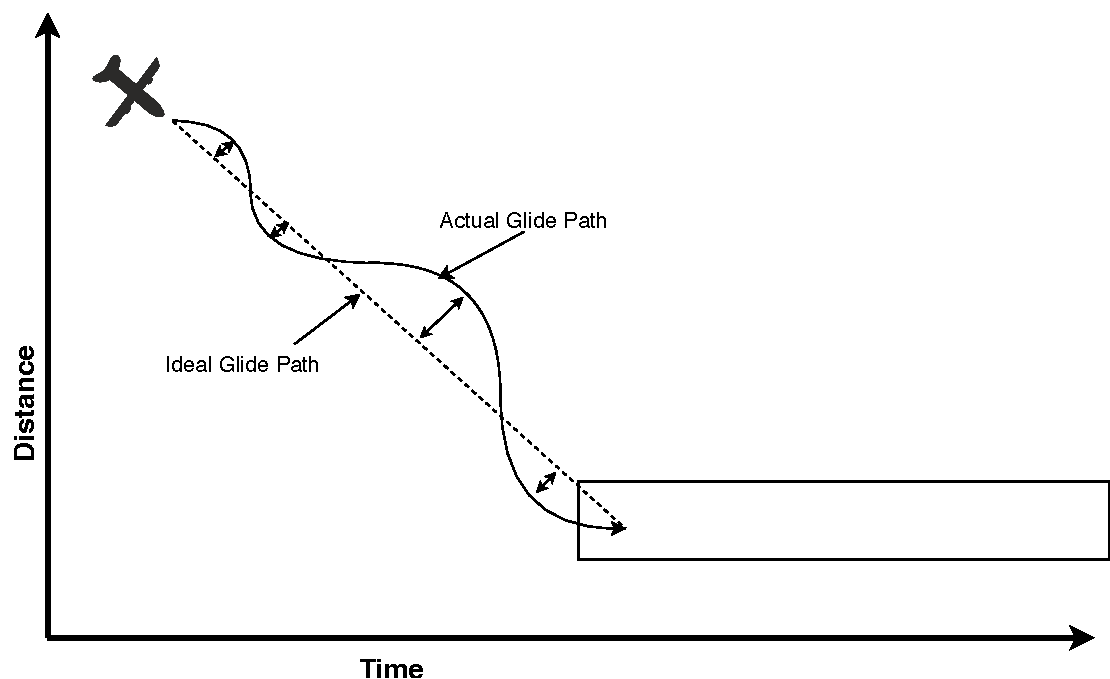
\includegraphics[width=\linewidth]{img/self_defined_example}
                \caption{Example showing the self-defined glide path angle analysis.  This shows a side view of the pilot oscillating about the glide slope during the approach phase.  The calculation uses a linear regression of the aircraft's vertical distance over time fitted using the least squares approach.  The solid line is the aircraft's actual glide path while the dotted line is the ideal glide path.}
                \label{fig:self_defined_example}
            \end{figure}
            
            
            %%%%% Analyze Self-Defined Glide Path Pseudo-code
            \begin{algorithm}[t]
                \begin{algorithmic}[1]\raggedright
                \Function{AnalyzeGlidePath}{startTime, endTime, runway}
                    \State $ \var{approachDataSlice} \gets $ get slice of data between the approach \var{startTime} and \var{endTime}
                    
                    \State $ \var{regressionResult} \gets \var{linearRegression(} \break \var{approachDataSlice[`time'], approachDataSlice[`agl'])} $
                    \State $ \var{yIntercept} \gets \var{regressionResult.intercept} $
                    \State $ \var{slope} \gets \var{regressionResult.slope} $
                    
                    \State $ \var{maxDistance} \gets \var{max(approachDataSlice[`distance'])} $
                    \State $ \var{minDistance} \gets \var{min(approachDataSlice[`distance'])} $
                    \State $ \var{horizontalDistance} \gets \var{maxDistance} - \var{minDistance} $
                    
                    \State $ \var{maxTime} \gets \var{max(approachDataSlice[`time'])} $
                    \State $ \var{minTime} \gets \var{min(approachDataSlice[`time'])} $
                    
                    \State $ \var{predictedMaxAGL} \gets \var{slope} * \var{maxTime} + \var{yIntercept} $
                    \State $ \var{predictedMinAGL} \gets \var{slope} * \var{minTime} + \var{yIntercept} $
                    
                    \State $ \var{predictedVerticalDistance} \gets \var{predictedMaxAGL} - \var{predictedMinAGL} $
                    
                    \State $ \var{actualGlidePathAngle} \gets \var{degrees(} \break \var{atan(predictedVerticalDistance / horizontalDistance))} $
                    
                    \State $ \var{pearsonsR} \gets \var{regressionResult.rvalue} $
                    \State $ \var{rSquared} \gets \var{pearsonsR} * \var{pearsonsR} $
                    
                    \State $ \var{approaches[apprID]} \gets $ store self-defined glide path metadata
                    \State \Return \var{(actualGlidePathAngle, rSquared)}
                \EndFunction
                \end{algorithmic}
                \caption{Pseudo-code for function which analyzes the quality of the aircraft's glide path angle during the approach phase.}
                \label{alg:analyze_glide_path}
            \end{algorithm}
    

%----------------------------------------
% GRADING METRICS
%----------------------------------------
\section{Grading Metrics}
    
    When creating the risk level metrics to be used for grading the approach analysis data, we wanted to ensure they were backed by statistics obtained from the results from the sample set of flights.  Towards that goal, the risk level metrics have been created from the data found during the approach quality analysis.  For each parameter of concern, the recorded values across all approach phases in the sample set were used to create a normalized histogram showing the probability density of each value range.  From these histograms, the mean and standard deviation were calculated in order to create a best-fit line to overlay the histogram.  The charts were then analyzed by an aviation statistics expert at the University of North Dakota who gave his opinion on reasonable values to use for Risk Level 1 and 2 value ranges based on each mean, standard deviation, and best-fit line.  Even though those elements were created from the analysis statistics, the aviation expert wanted to also ensure the safe value ranges (Risk Level 0) did not conflict with the values published in UND's standardization manual~\cite{und_flight_manual} and the Cessna C172S Pilot's Operating Handbook (POH)~\cite{und_poh}.
    
    After the risk level metrics have been established, the approach quality analysis results will be re-processed and graded according to the metrics.  The resulting grade is then stored along with the other generated approach analysis data within the database.  The specific details of the grading results from using the risk level metrics will be discussed further in \Cref{ch:results}.
    
    
%----------------------------------------
% WEB INTERFACES
%----------------------------------------
\section{Web Interfaces}

	This Section details the newly developed web pages for the NGAFID, which dynamically display results based on the user's chosen filters.  At the time of this writing, there have been new tools developed for each of the approach, final turn, and self-defined glide path analyses.  Each tool will be discussed further in the subsequent Subsections.
    
    
    %----------
    % APPROACH
    %----------
    \subsection{Approach}
    
    	A new web page was implemented in the NGAFID for the purpose of dynamically displaying the approach analysis results produced by the \toolname\ to users (\Cref{fig:approach_tool_screenshot}).  The results are given in four tabs, one for each parameter, as histograms over a specified date range.  A user is able to dynamically add additional date ranges, which will create an additional series in the chart for comparison.  This feature can be used to detect changes in trends over time.  A user is also, optionally, able to filter the results to an airport and further filter to a single runway.  This will allow users to identify trends that are potentially occurring at a specific runway but not at any other runways.
    
    	\begin{figure}
    		\centering
            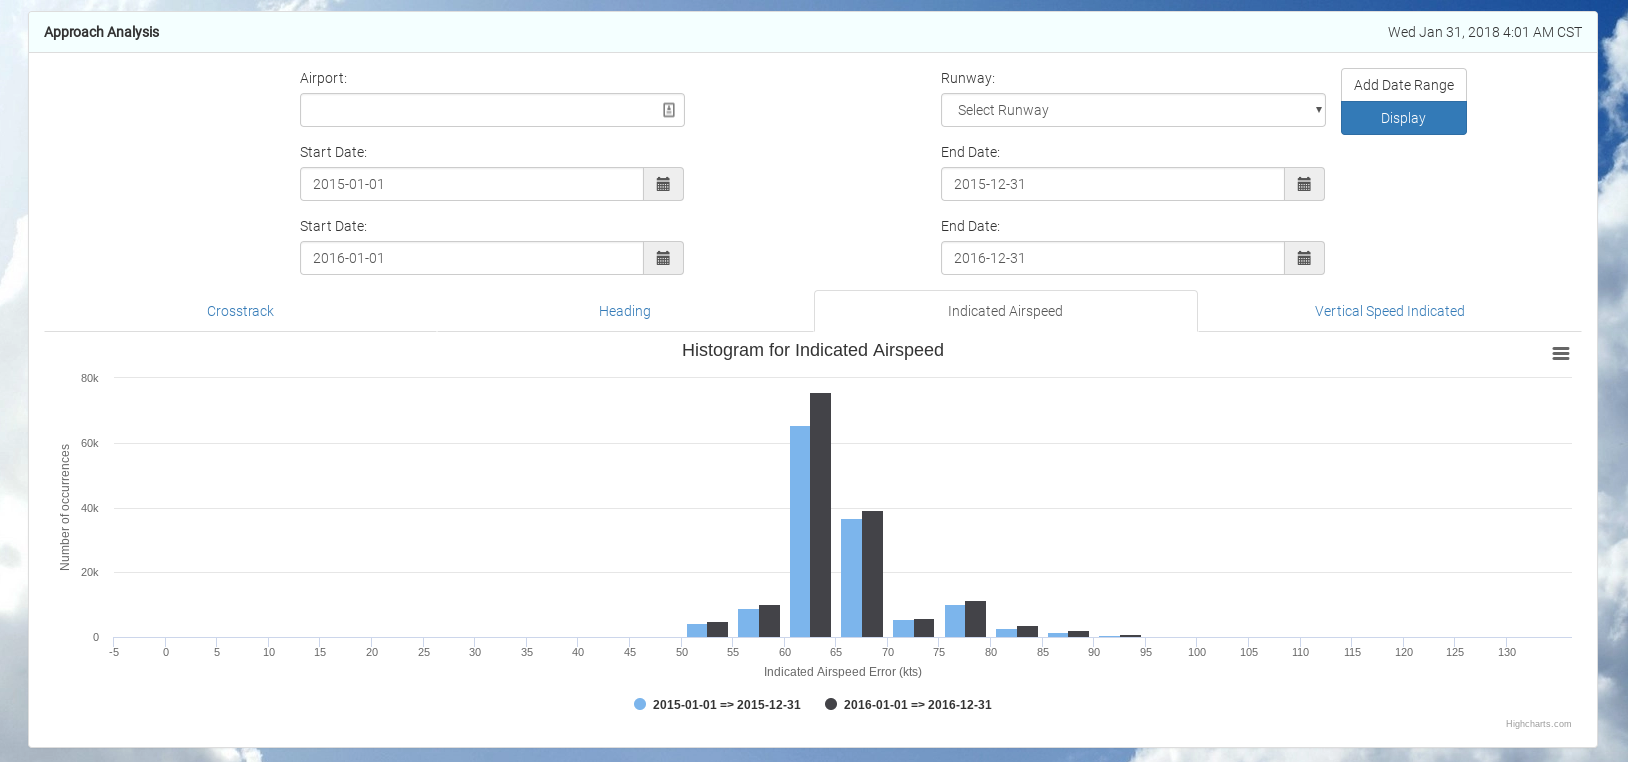
\includegraphics[width=\linewidth]{img/approach_tool_screenshot}
            \caption{A screenshot of the Approach analysis tool on the NGAFID.  It is showing the histogram for indicated airspeed error with two date range filters: 2015-01-01 to 2015-12-31 and 2016-01-01 to 2016-12-31.  The frequency of exceedances can be seen with all values that fall outside of the 55-75 knots range.}
            \label{fig:approach_tool_screenshot}
    	\end{figure}
    
    
    %----------
    % FINAL TURN
    %----------
    \subsection{Final Turn}
    
    	The tool developed for analyzing final turn phases in the NGAFID was implemented with two modes:  \textit{(i)} ``Single Flight'' and \textit{(ii)} ``Aggregate''.
    
    	For the ``Single Flight'' mode, the user can input an ID for a specific flight they'd like to analyze (\Cref{fig:single_ttf_screenshot}).  Once the user clicks the ``Display Single Flight'' button, the interactive map then dynamically transitions to the first approach for that flight.  The map will only display one approach at a time; although, there are tabs across the top for each approach which the user can choose.  Once a different tab is chosen, the map automatically transitions the view to that corresponding approach.  The flight path shows different color codings for the separate final turn, approach, and landing phases as well as different colors for the final turn specifically depending on the severity of the turn error.  A Level 1 turn error will be colored yellow, while a Level 2 turn error will be colored red.  If the turn error is less than the Level 1 criteria, it is colored green.  The user is also able to download a PNG screenshot of the map by clicking the ``Download PNG'' button.
        
        For the ``Aggregate'' mode; the user can choose a specific airport, runway, and month and year combination; which will then display all the approaches that occurred at the chosen runway during the chosen time-frame (\Cref{fig:agg_ttf_screenshot}).  This mode allows a user to see trends in final turn phases during a given time span.  This mode displays the same color code scheme as the ``Single Flight'' mode.
    
    	\begin{figure}
    		\centering
            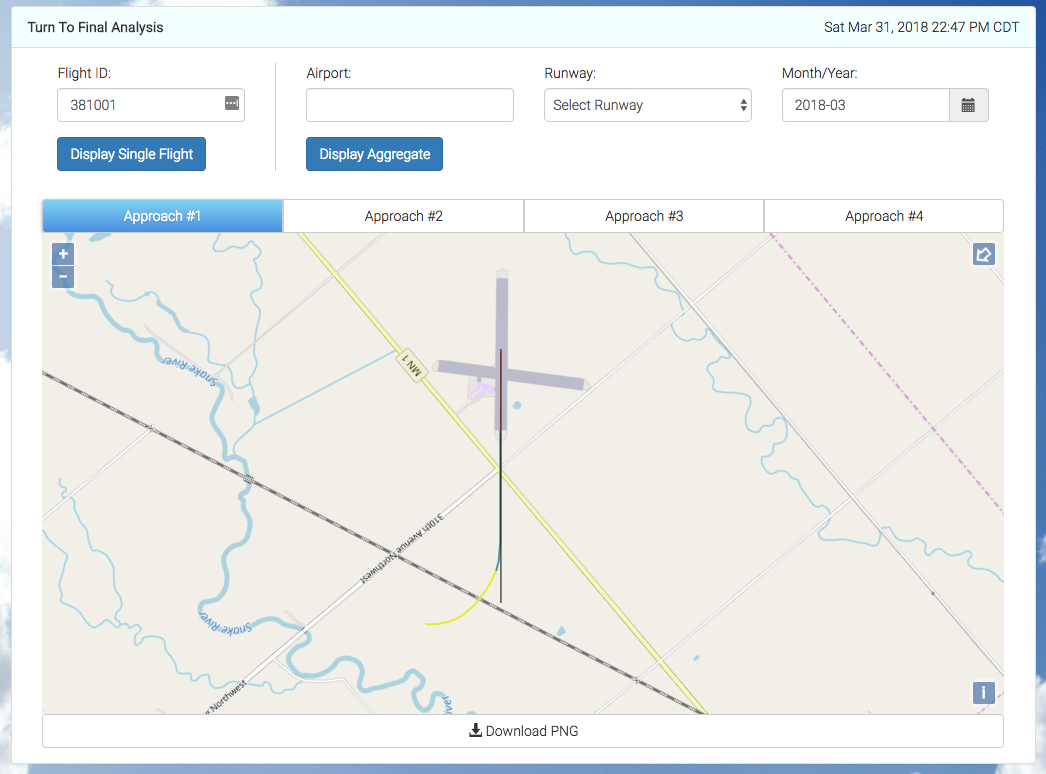
\includegraphics[width=\linewidth]{img/single_ttf_screenshot}
            \caption{A screenshot of the Final Turn analysis tool on the NGAFID in ``Single Flight'' mode.  It is currently showing approach \#1 for Flight ID \#381001.  Approach \#1 shown here had a Level 1 (yellow color code) undershoot.}
            \label{fig:single_ttf_screenshot}
    	\end{figure}
        
        \begin{figure}
    		\centering
            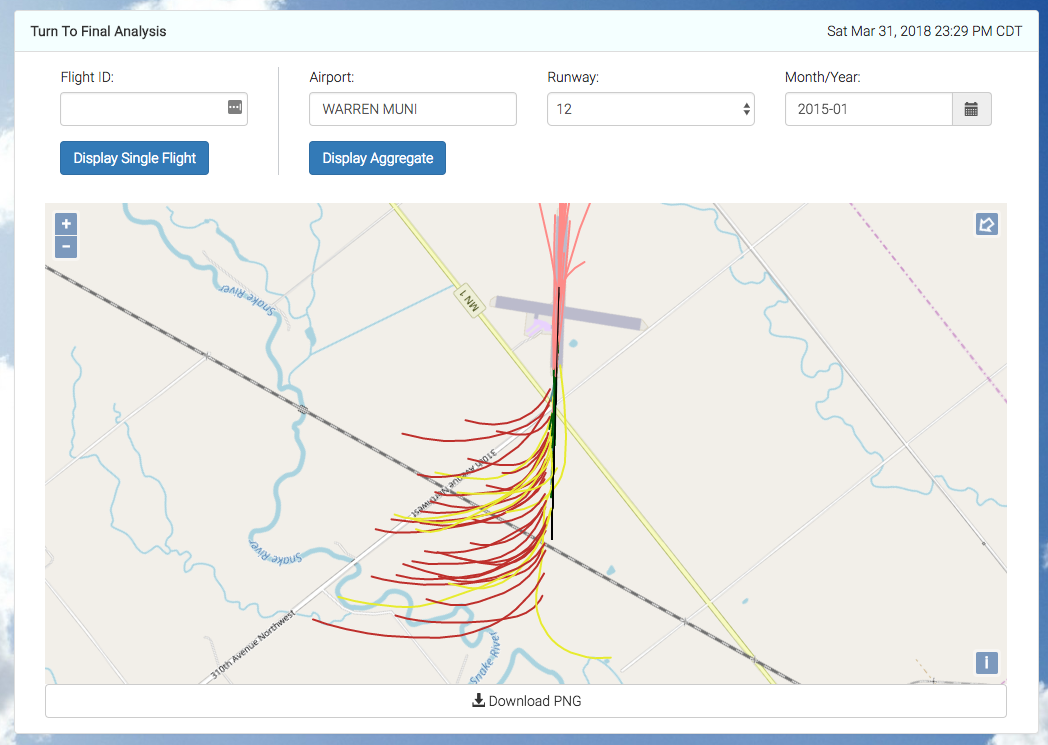
\includegraphics[width=\linewidth]{img/agg_ttf_screenshot}
            \caption{A screenshot of the Final Turn analysis tool on the NGAFID in ``Aggregate'' mode.  It is currently showing all approaches at the Warren Municipal Airport (KD37) for Runway 12 during the month of January 2015.  The many red and yellow lines coming in from the left side mean that a majority of the turns were Level 1 \& 2 undershoots.}
            \label{fig:agg_ttf_screenshot}
    	\end{figure}
    
    %----------
    % SELF-DEFINED
    %----------
    \subsection{Self-Defined Glide Path}
    
    	The tool implemented in the NGAFID for displaying the results of the self-defined glide path analysis currently only supports an aggregate mode (\Cref{fig:self_defined_screenshot}).  It works similarly to the final turn tool as the user chooses an airport, runway, and month and year combination.  This will then display a sideways histogram of all the approaches at the given runway during the given time-frame.  The y-axis shows glide path angles from $0^\circ$ to $10^\circ$ in $0.5^\circ$ increments, and the x-axis shows the number of occurrences that fell within each angle bin.  Lastly, the user can download an image of the displayed chart by clicking the ``hamburger'' menu button.
    
    	\begin{figure}
    		\centering
            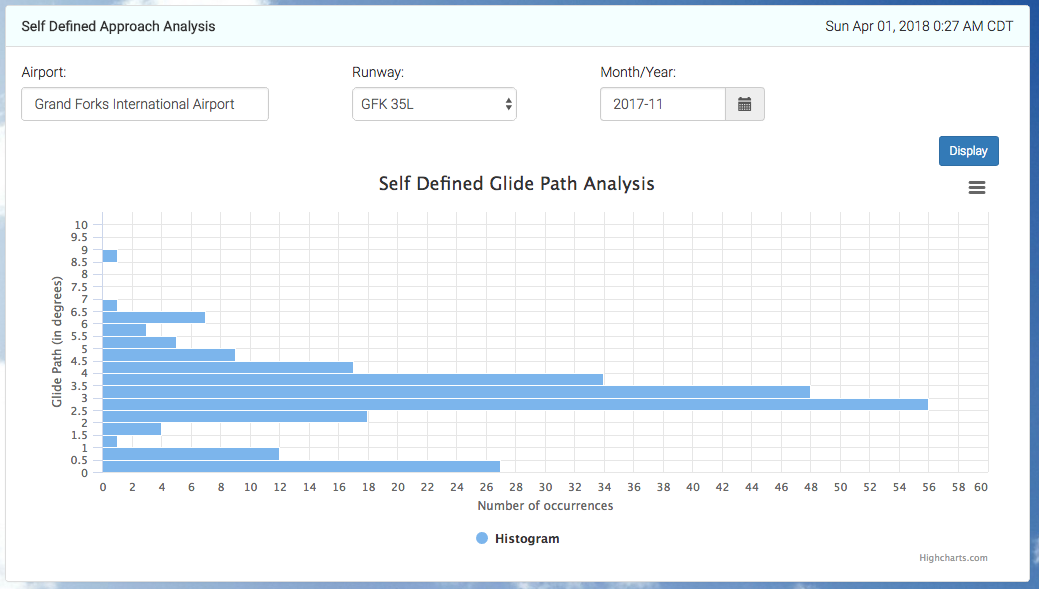
\includegraphics[width=\linewidth]{img/self_defined_screenshot}
            \caption{A screenshot of the Self-Defined Approach analysis tool on the NGAFID.  It is currently showing all approaches at the Grand Forks International Airport (KGFK) for Runway 35L during the month of November 2017.  It displays a sideways histogram with glide path angles on the y-axis and the number of occurrences for each angle on the x-axis.}
            \label{fig:self_defined_screenshot}
    	\end{figure}



\chapter{Implementation} \label{ch:implementation}

%----------------------------------------
% PROGRAMMING LANGUAGES & LIBRARIES
%----------------------------------------
\section{Programming Languages and Libraries}

	The Python programming language was used for implementing the flight analysis due to its ease of use, its reputable scientific and graphing libraries, and the ability to quickly produce a viable application.  The libraries utilized are MySQLdb\footnote{http://mysql-python.sourceforge.net/MySQLdb.html} for interacting with the MySQL database, matplotlib\footnote{https://matplotlib.org/} for graphing flight parameters in the early stages of the application, NumPy\footnote{http://www.numpy.org/} and Pandas\footnote{https://pandas.pydata.org/} for their scientific functions, and the geodesy scripts created by Chris Veness\footnote{http://www.movable-type.co.uk/scripts/latlong.html}.  All source code is available at \url{https://github.com/KeltonKarboviak/NGAFID}.
    
    For web interface\todo{Fix this.}: Laravel 5.0\footnote{https://laravel.com/} as a PHP back-end framework, jQuery 2.2.4\footnote{https://jquery.com/} \& jQuery UI 1.11.2\footnote{https://jqueryui.com/}, Bootstrap 3\footnote{https://getbootstrap.com/docs/3.3/} for CSS styling, OpenLayers 4.6.4\footnote{http://openlayers.org/} for creating an interactive map, OpenStreetMap\footnote{https://www.openstreetmap.org} for the images used by OpenLayers, and Turf.js 5.1.5\footnote{http://turfjs.org/} for its geodesy functions.  All source code for the web interface is available at \url{https://github.com/travisdesell/ngafid}.


%----------------------------------------
% HARDWARE SPECS
%----------------------------------------
\section{Hardware Specs}

	All experiments were performed on a 2013 Mac Pro running macOS 10.11.6 with a 3.5 GHz 6 hyper-threaded core Intel Xeon E5 processor (for a total of 12 logical processing cores). The machine also has 32 GBs of 1866 MHz DDR3 ECC RAM.


%----------------------------------------
% PARALLELIZATION
%----------------------------------------
\section{Parallelization}

	The application was originally created to process the flight data in a linear fashion.  This proved to be fairly time consuming when running the application in batch mode with the significant number of flights contained in the NGAFID.  In order to improve the performance and efficiency of the application, Python's built-in multiprocessing module was used.  The parallel application uses the simple Producer-Consumer model in which the parent process acts at the Producer by enqueuing all of the unique flight identifiers onto a queue and the child subprocesses act as the Consumers by dequeuing a flight identifier then processing it.  The multiprocessing module was chosen over the built-in threading module due to the issue with Python's Global Interpreter Lock (GIL) effectively restricting bytecode execution to a single core~\cite{Beazley:2010:Understanding-t}.  This makes the threading module unusable for long-running CPU-bound tasks, which this application heavily relies on.
% !TEX root = ../main.tex

\chapter{Results} \label{ch:results}

%----------------------------------------
% EXPERIMENTS
%----------------------------------------
\section{Experiments}

	The experiments were run using Cessna 172S flight data produced by students at the University of North Dakota during the month of September 2015.  Student flight data is ideal for unstable analysis testing as it contains very noisy data, which provides a diverse array of flying patterns.  A random sample of 100 flights was chosen for the experiments.
        
    First, the application was run against the 100 flights to obtain the automated analysis results.  The same 100 flights were then manually analyzed in order to get human results for the phase identification, which could be compared to the automated results then determine the accuracy of the application.  The test of the 100 flights was also run ten times each with the single-process version and the multi-process version as previously described.  This was done in order to compare and contrast the performance of the separate versions.


%----------------------------------------
% ACCURACY OF PHASE IDENTIFICATION
%----------------------------------------
\section{Accuracy of Phase Identification}

	The manual validation was performed using a combination of tools available on the NGAFID website:  the Cesium flight reanimation tool and the Keyhole Markup Language (KML) generator to visualize the flight path in \textit{Google Earth}~\cite{nolan2014keyhole} (see \Cref{fig:kml_example}).
    
    \begin{figure}
    	\centering
        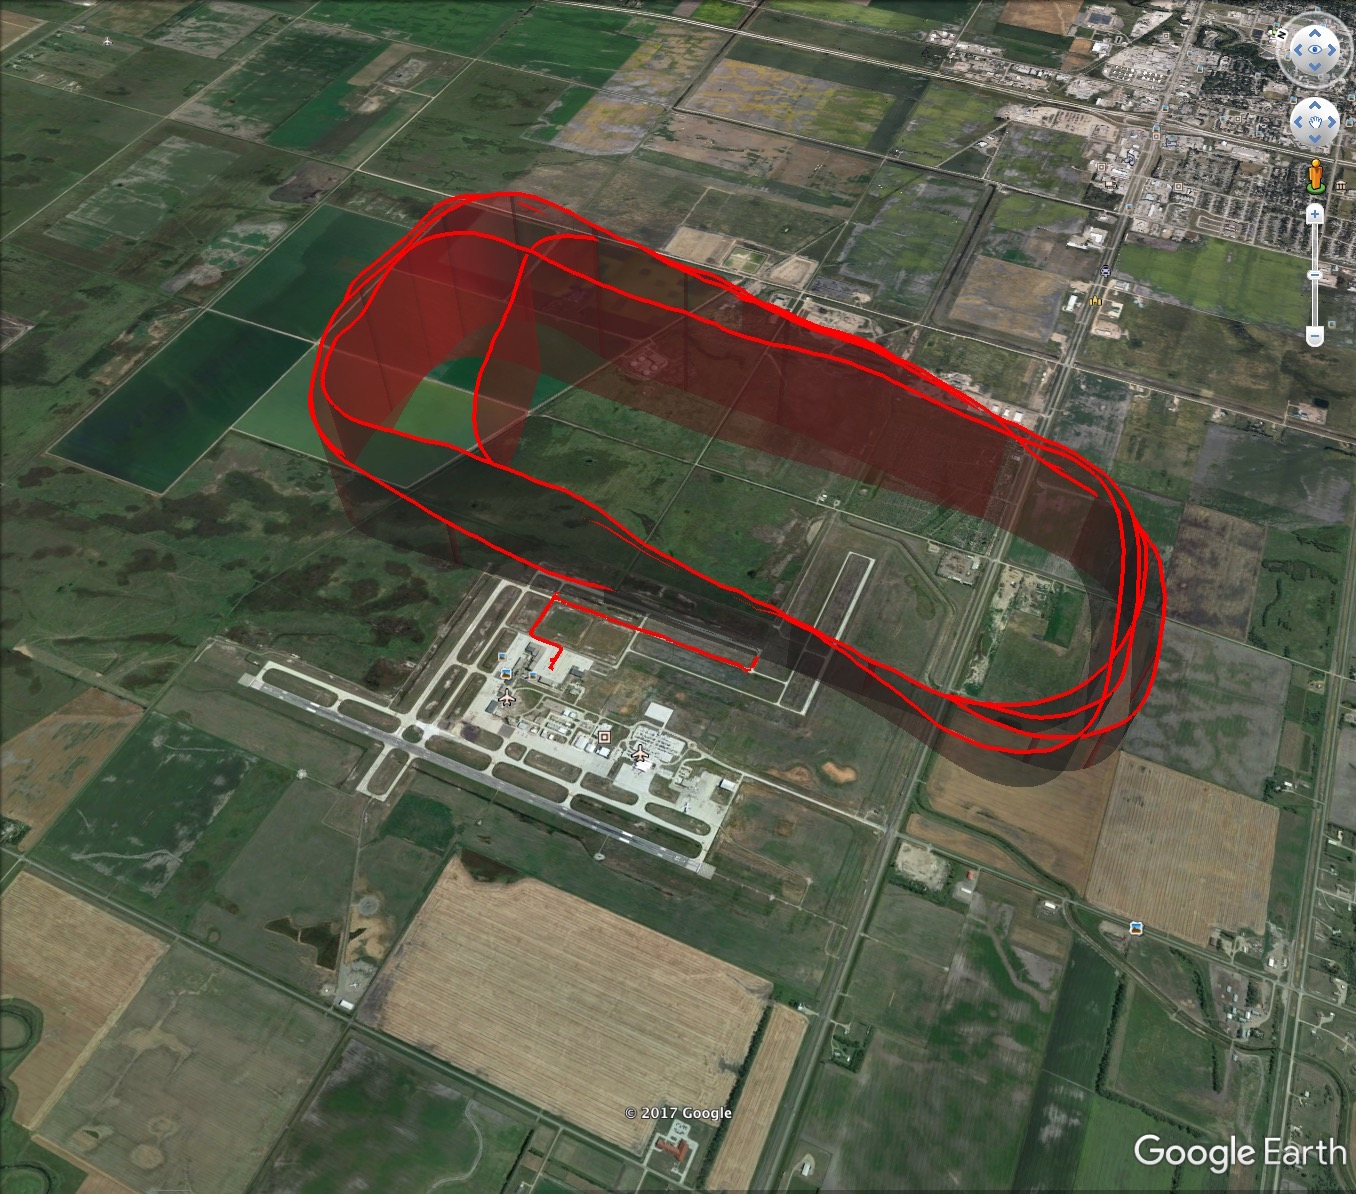
\includegraphics[width=\linewidth]{img/kml_example}
        \caption{Example of using a KML file to visualize a flight path in \textit{Google Earth}.  This flight visualization is an example of a student flight that has multiple Approach phases.}
        \label{fig:kml_example}
    \end{figure}
    
    
    %----------
    % APPROACH
    %----------
    \subsection{Approach}
    
        The \toolname\ generated a total of 380 approaches for the 100 flights that were tested. As seen in \Cref{fig:kml_example}, student flights typically consist of multiple approaches as this is something that needs to be practiced.  Out of the total; there are 3730 (98.16\%) true positives, five (1.32\%) false positives, and two (0.53\%) false negatives.  These results can also be found in \Cref{fig:validation_results}.
        
        In the context of this application, a true positive is a case where the tool correctly indicates that an approach is occurring during a specified time frame.
        
        A false positive occurs when the tool indicates that an approach is occurring but is not in reality.  Typically, a false positive occurs when the flight data has invalid values for about the first ten rows, which then throws off the beginning of the algorithms.  This happens infrequently, but could be accounted for in a future work by sanitizing the data before analysis.
        
        A false negative is the exact opposite where the tool indicates that an approach is not occurring but it is in reality.  Typically, a false negative occurs when the approached runway's geological data is not contained within the database.  These types of occurrences should stop once the airport and runway databases are expanded with more entries.
        
        The tool misclassified the approached runway 13 times (3.42\%).  A runway is misclassified when the difference between the aircraft and runway headings is greater than $20^\circ$.  This occurs during the runway detection portion of the approach analysis algorithm, and the algorithm either returns a \emph{null} runway or an incorrect runway due to the large heading difference.  Lastly, there was a total of 42 (11.05\%) approaches that were given a \textit{null} runway.  This number overlaps with some of the 13 misclassifications, while the rest are due to a lack of runway information as mentioned previously.

        In this same context, it is difficult to quantify the number of true negatives since these would be cases where the tool correctly indicates that an approach is not occurring.  The difficulty lies in how to define a single occurrence.  Should a single true negative be counted for every second the tool indicates that an approach is not occurring?  If so, then this would create a numerous amount of true negatives and would dilute the percentages of the other statistics, which are more important in this application.

        The validation results demonstrate that the \toolname\ is exceptionally accurate in its ability to appropriately detect and classify most approaches in a flight.

        \begin{figure}
            \centering
            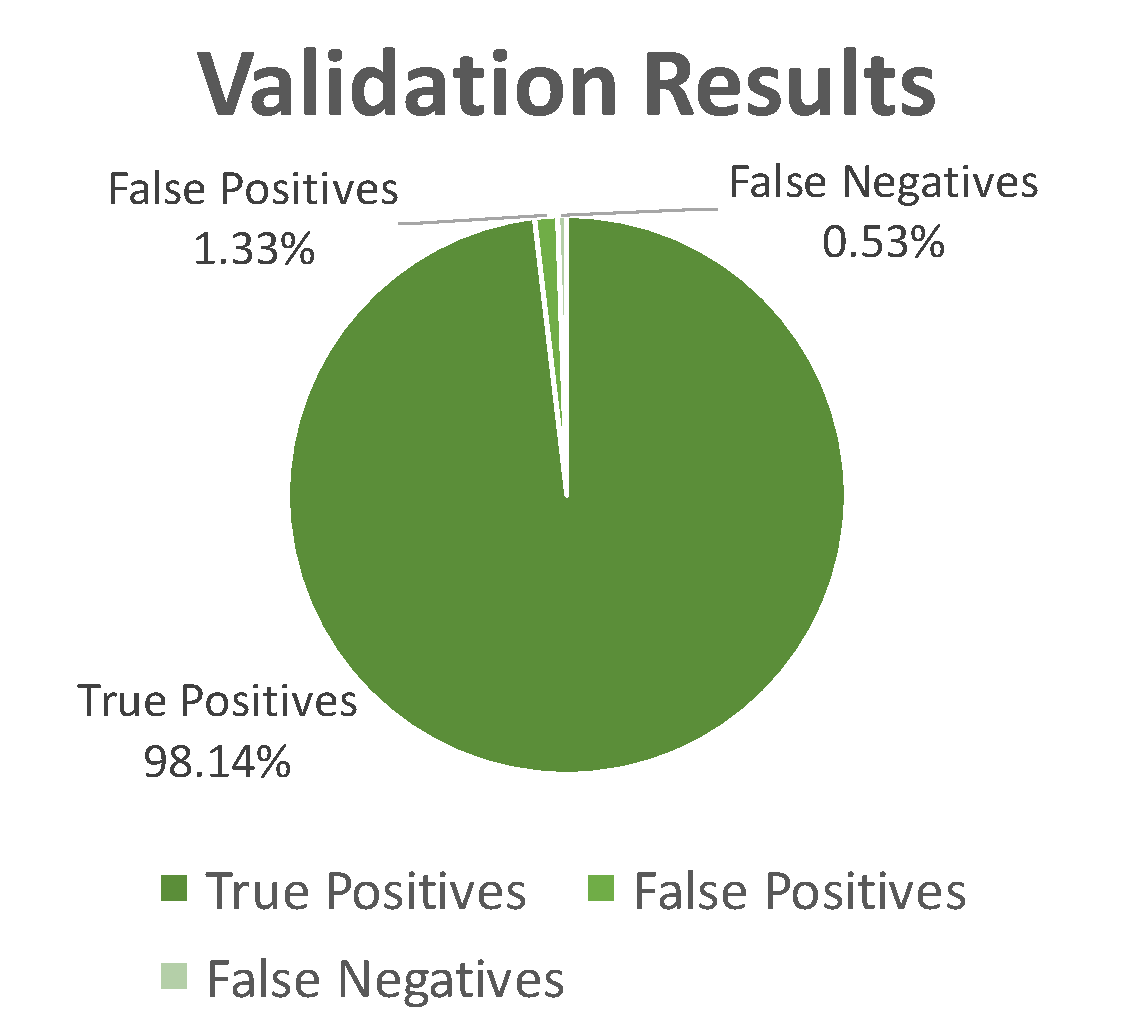
\includegraphics[width=0.75\linewidth]{validation_results}
            \caption{Pie chart showing the manual validation results including true positives, false positives, and false negatives.}
            \label{fig:validation_results}
        \end{figure}
    
    
%----------------------------------------
% QUALITY ANALYSIS RESULTS
%----------------------------------------
\section{Quality Analysis}


	%----------
    % APPROACH
    %----------
    \subsection{Approach}
    
    	The results of the application have provided many possibilities for statistical analysis since numerous statistics can be calculated from the generated approach data.  This can be seen in \Cref{subfig:stableness_results,subfig:unstable_landing_results,subfig:unstable_parameters,subfig:landing_type_results} in which a sample of the possible results were calculated from the experiments of the 100 flights used in this research.  With these various results, trends can be found in the data that has been analyzed.  For example, we can see in \Cref{subfig:stableness_results} that out of the 380 approaches in the sample data, 57.11\% (217) were stable and 42.89\% (163) were unstable.  By drilling down into that data, we can see the frequency for each of the landing types for stable and unstable approaches.  \Cref{subfig:landing_type_results} depicts this more detailed information and shows that full-stop landings occur most frequently for both stable and unstable approaches.  This result is not very surprising for stable approaches; however, it is very undesirable for unstable approaches.  If we look even further into the proportions for unstable approaches alone (\Cref{subfig:unstable_landing_results}), we see that an unstable approach resulted in a go-around only 34.97\% of the time.  This is far lower than the hopeful 100\%, but was expected to be approximately 20\% by our aviation safety experts.  As mentioned previously, this is largely due to pilot misjudgment since all the analyzed flights were piloted by aviation students; meaning they are still learning and are not yet professionals.
    
    When looking at the unstable approaches and the parameters that caused them (\Cref{subfig:unstable_parameters}), additional interesting results can be found.  We found the parameter that was exceeded the most was heading with 91 occurrences.  Heading was not predicted to be the leading cause of unstable approaches, but our safety experts believe the 10$^\circ$ threshold (as defined in \Cref{tab:approach_thresholds}) may be too strict.  Indicated airspeed was the second highest, but was predicted to be the leading cause since it was stated by our aviation safety experts to be a trend for UND's student pilots to be going too fast on final approaches.
    
    \begin{figure}
    	\centering
        \subfloat[Pie chart showing the number of stable approaches compared to the number of unstable approaches.\label{subfig:stableness_results}]{
        	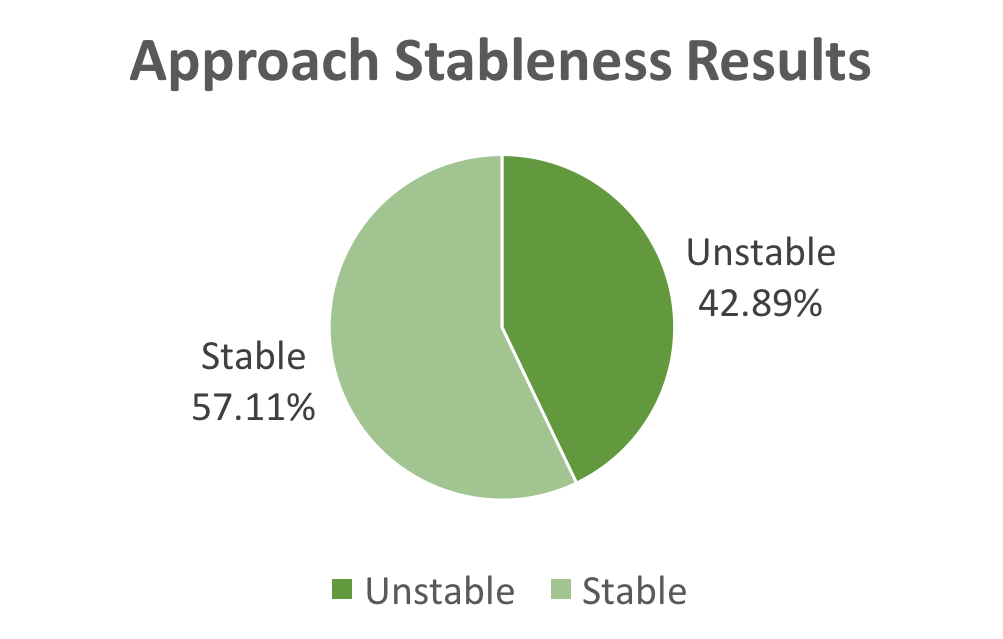
\includegraphics[width=0.45\linewidth]{stableness_results}
        }\hfill%
        \subfloat[Frequency of the occurrences of each landing type for stable and unstable approaches.\label{subfig:landing_type_results}]{
        	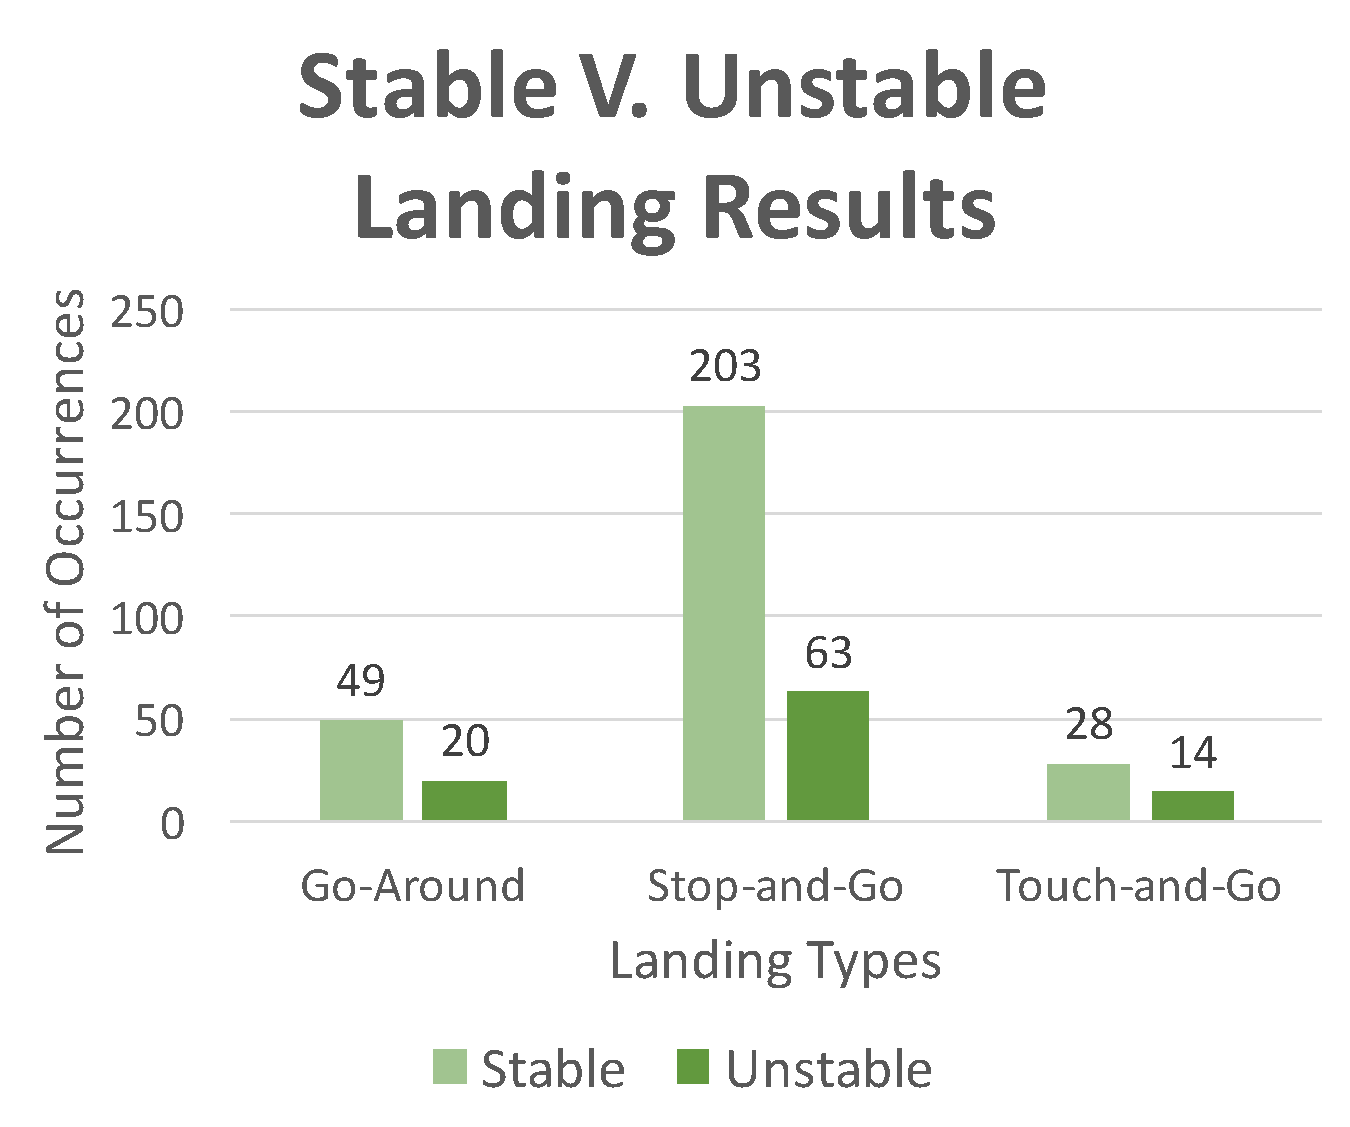
\includegraphics[width=0.45\linewidth]{landing_type_results}
        }%
        
        \subfloat[Pie chart comparing the number of occurrences for each landing type after an unstable approach.\label{subfig:unstable_landing_results}]{
        	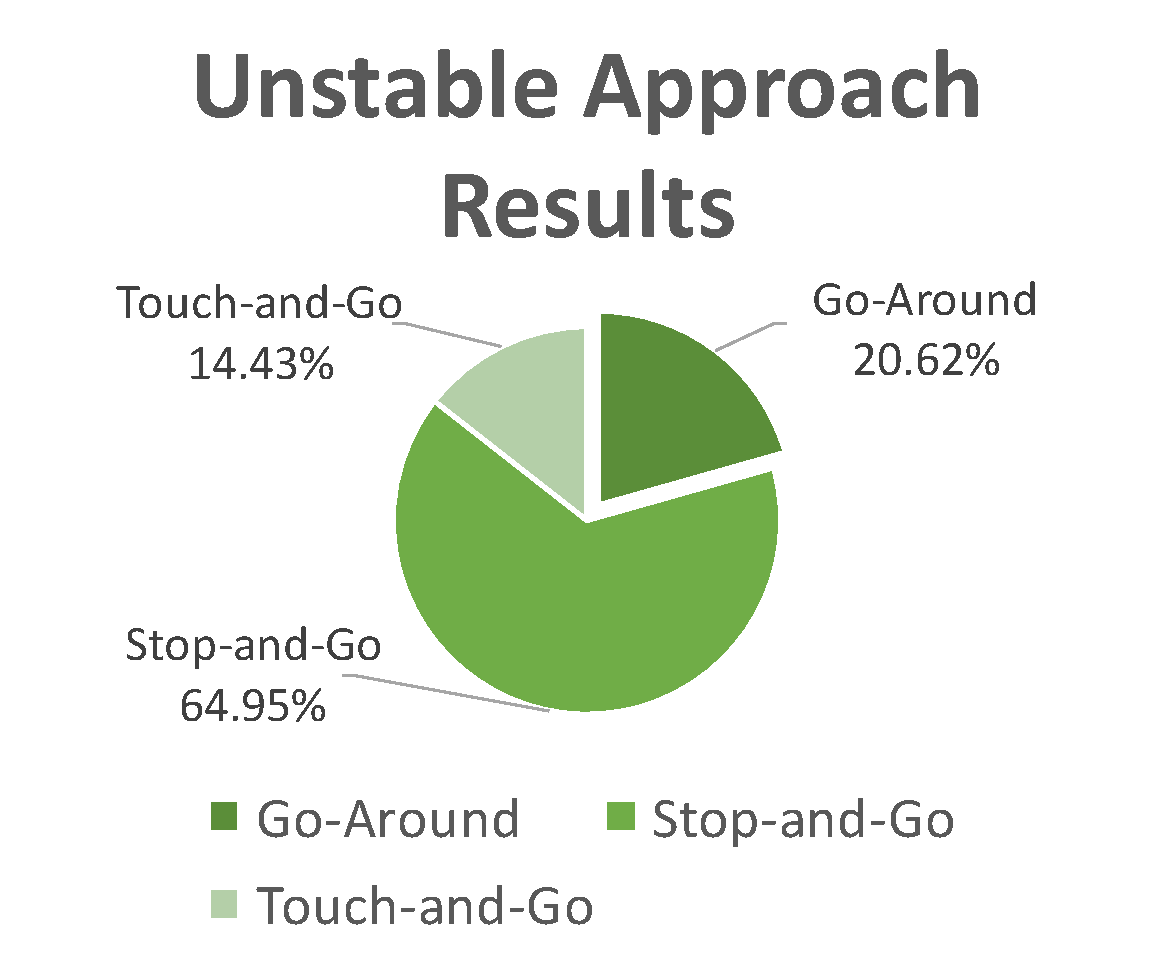
\includegraphics[width=0.45\linewidth]{img/unstable_approach_landing_results}
        }\hfill%
        \subfloat[Frequency of parameters that caused an aircraft to be unstable during an approach.  Note that a single approach can have multiple unstable parameters, which causes the sum of the occurrences to not equal the total number of unstable approaches.\label{subfig:unstable_parameters}]{
        	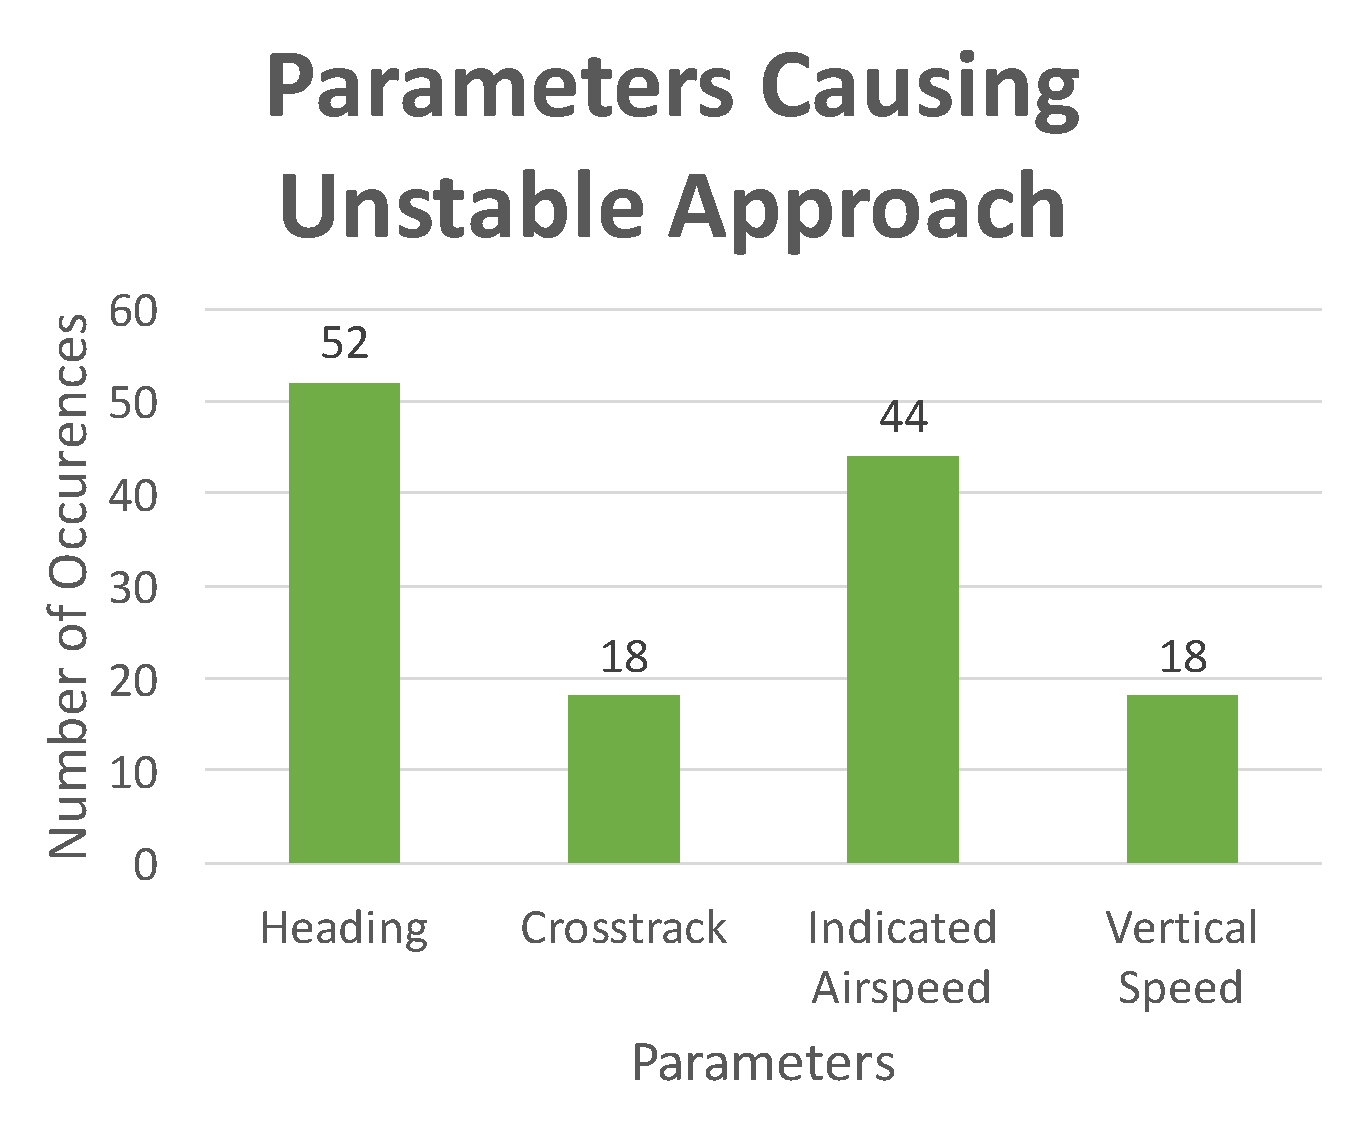
\includegraphics[width=0.45\linewidth]{unstable_parameter_results}
        }%
        \caption{Sample set of the statistics and trends that can be found from the automated analysis results.}
        \label{fig:example_statistics}
    \end{figure}
    
    
    Another interesting set of statistics that can be drawn from the analysis are parameter value frequencies.  Creating histograms of the values for each parameter during all Approach phases can show the values that occur most frequently (highest density).  \Cref{subfig:approach_ias_hist,subfig:approach_vsi_hist,subfig:approach_cross_track_hist,subfig:approach_heading_hist} visualize these histograms and give the corresponding mean and standard deviation values.  These graphs are able to show how well pilots are adhering to the published stabilized approach criteria (see \Cref{tab:approach_thresholds}).  As mentioned previously, the standard deviations will be used in defining the grading metrics and will be discussed in more detail later in this Chapter.
    
    \begin{figure}
    	\centering
        \subfloat[Indicated airspeed.\label{subfig:approach_ias_hist}]{
        	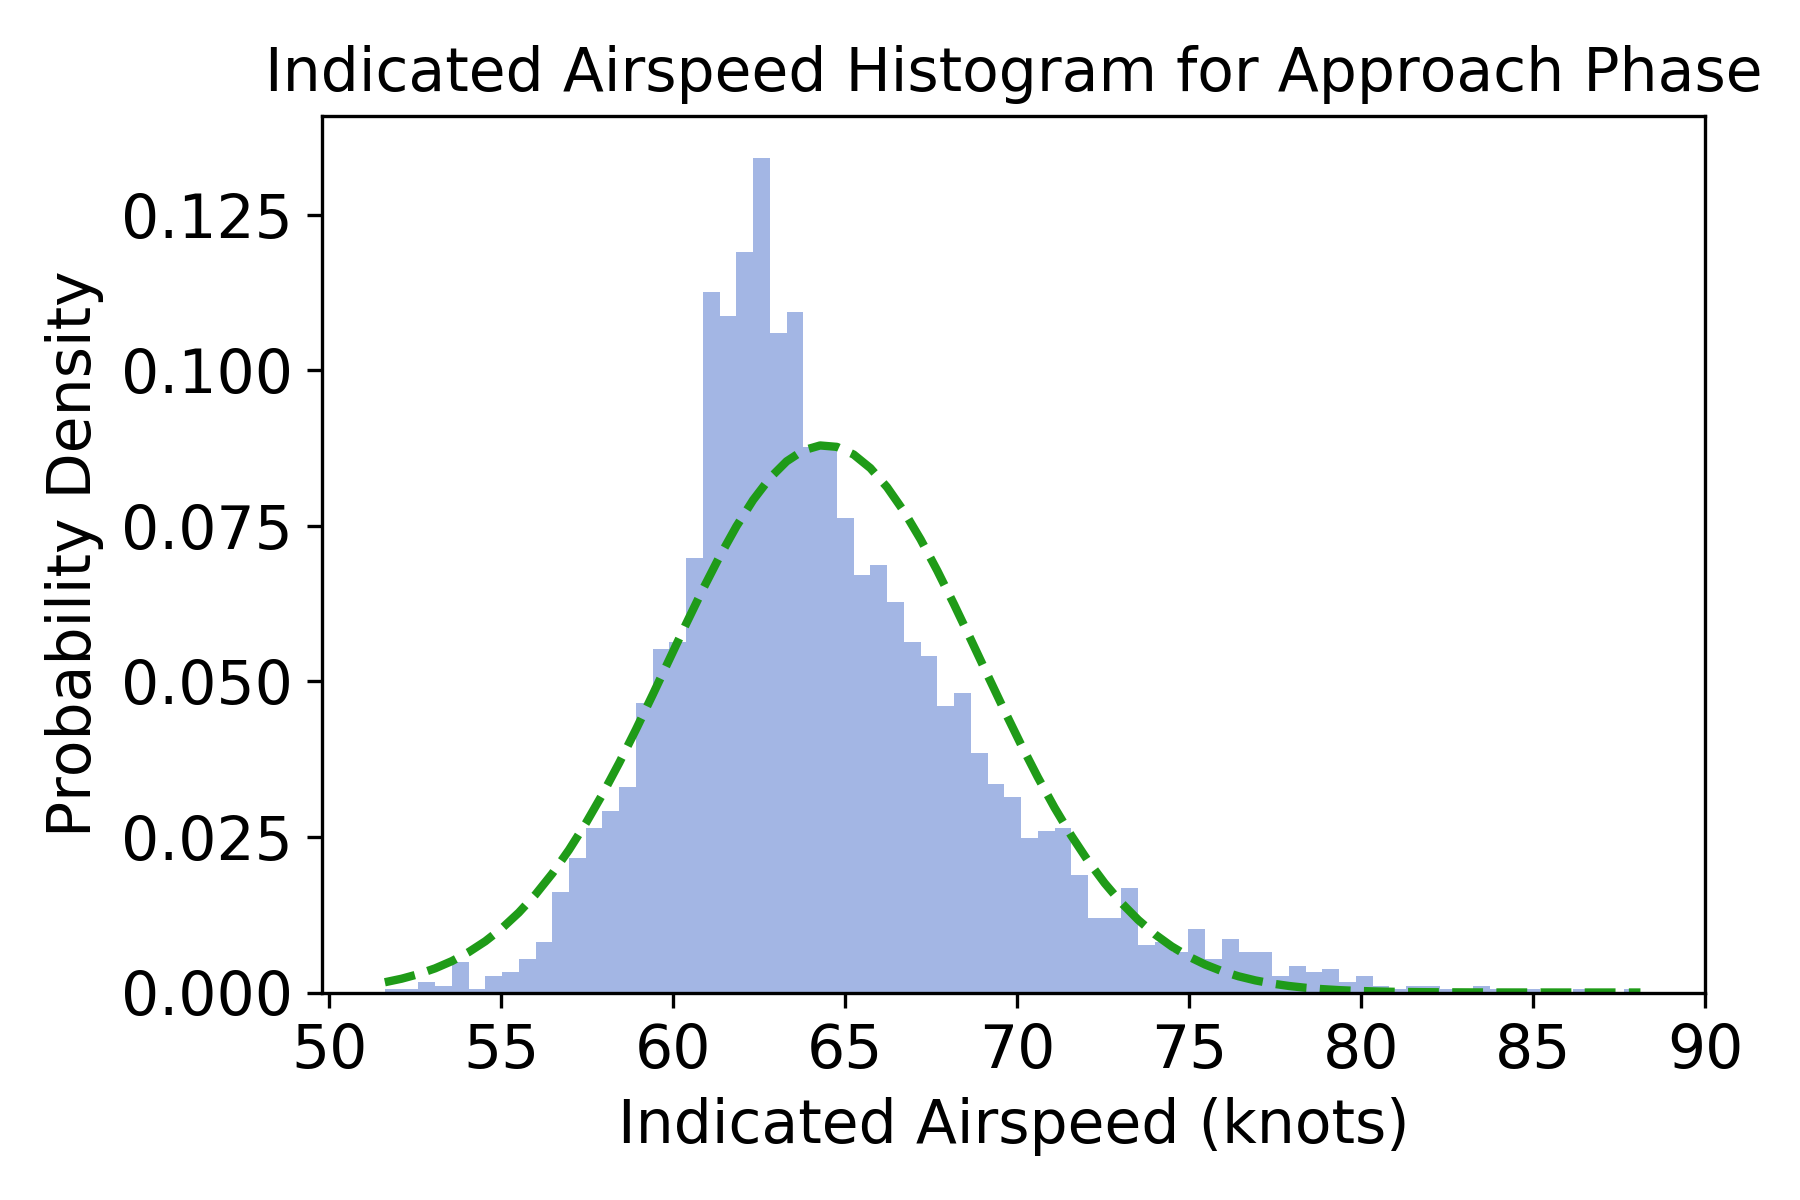
\includegraphics[width=0.45\linewidth]{orig_ias_hist}
        }\hfill%
        \subfloat[Vertical speed indicated.\label{subfig:approach_vsi_hist}]{
        	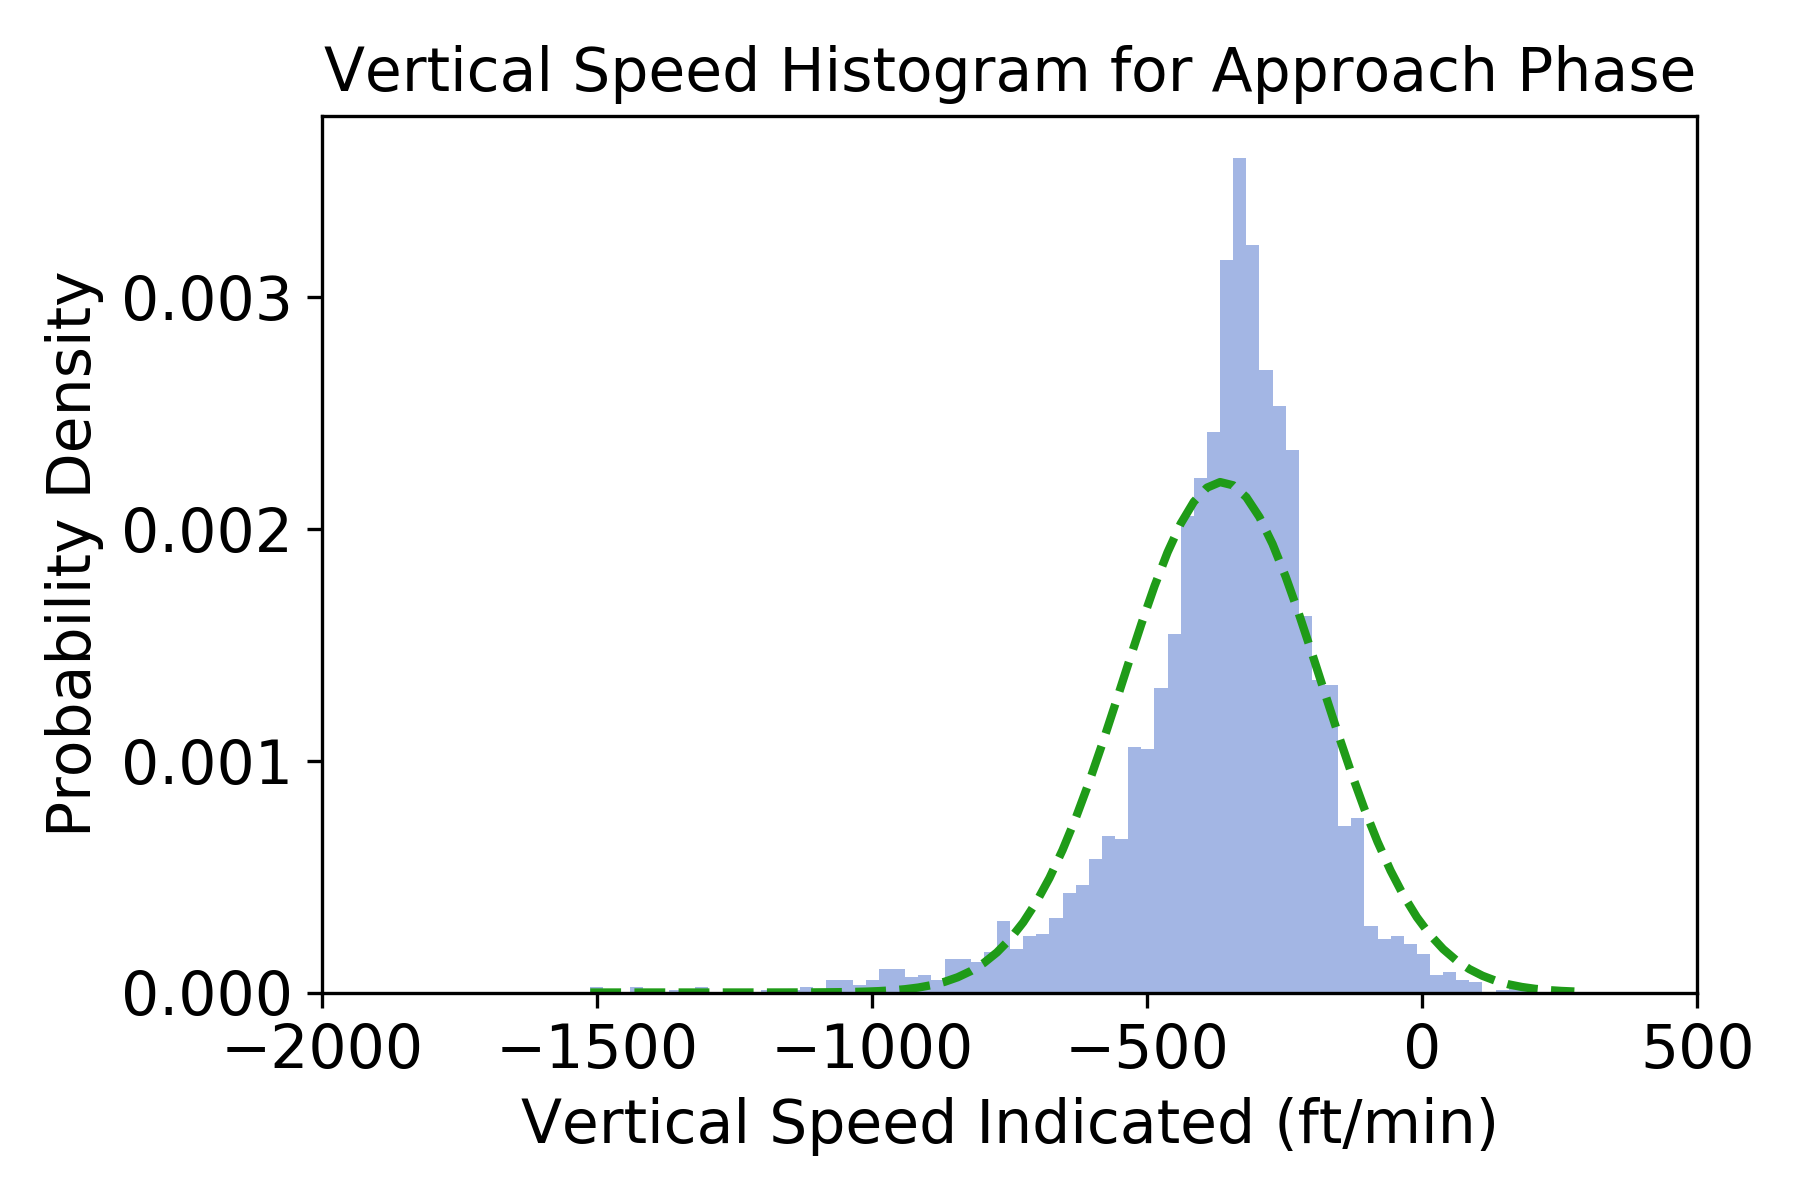
\includegraphics[width=0.45\linewidth]{orig_vsi_hist}
        }%
        
        \subfloat[Cross track error.\label{subfig:approach_cross_track_hist}]{
        	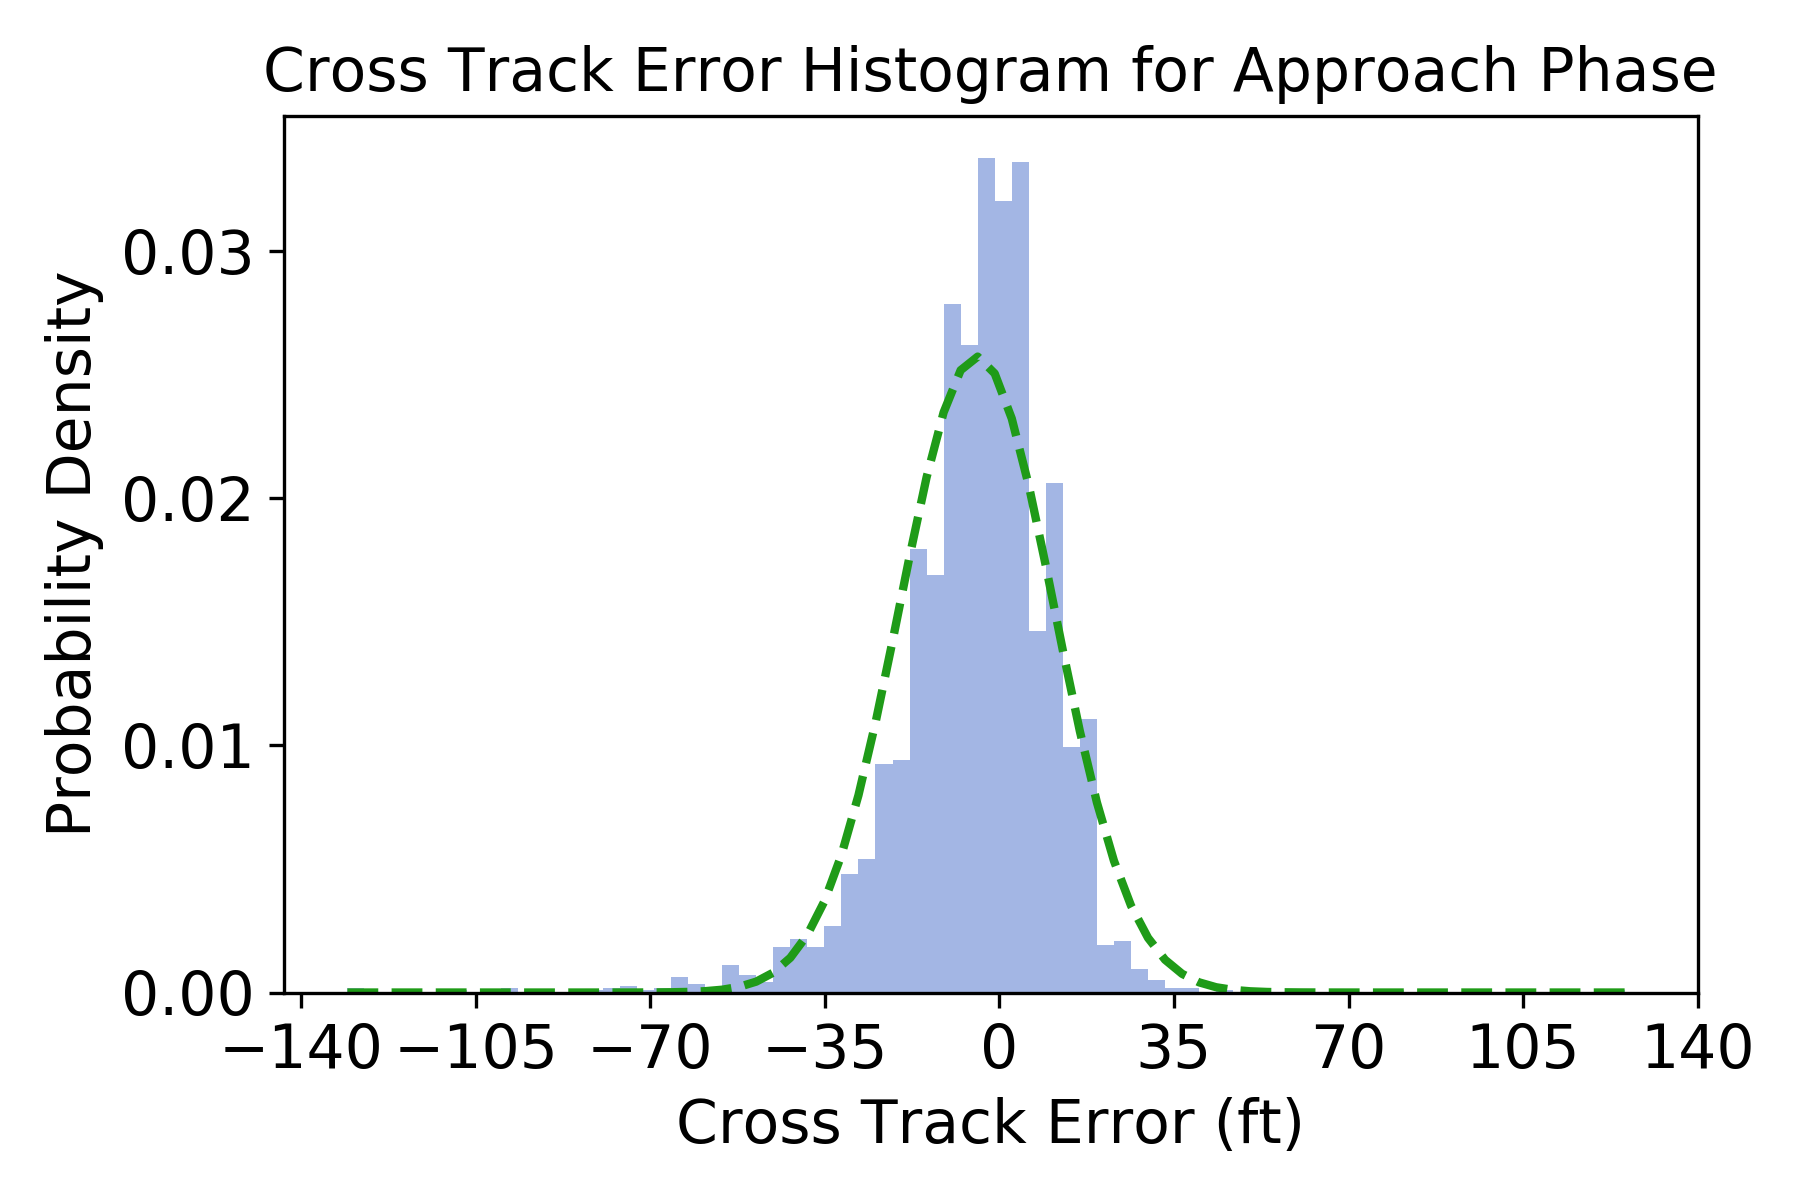
\includegraphics[width=0.45\linewidth]{orig_cross_track_hist}
        }\hfill%
        \subfloat[Heading error.\label{subfig:approach_heading_hist}]{
        	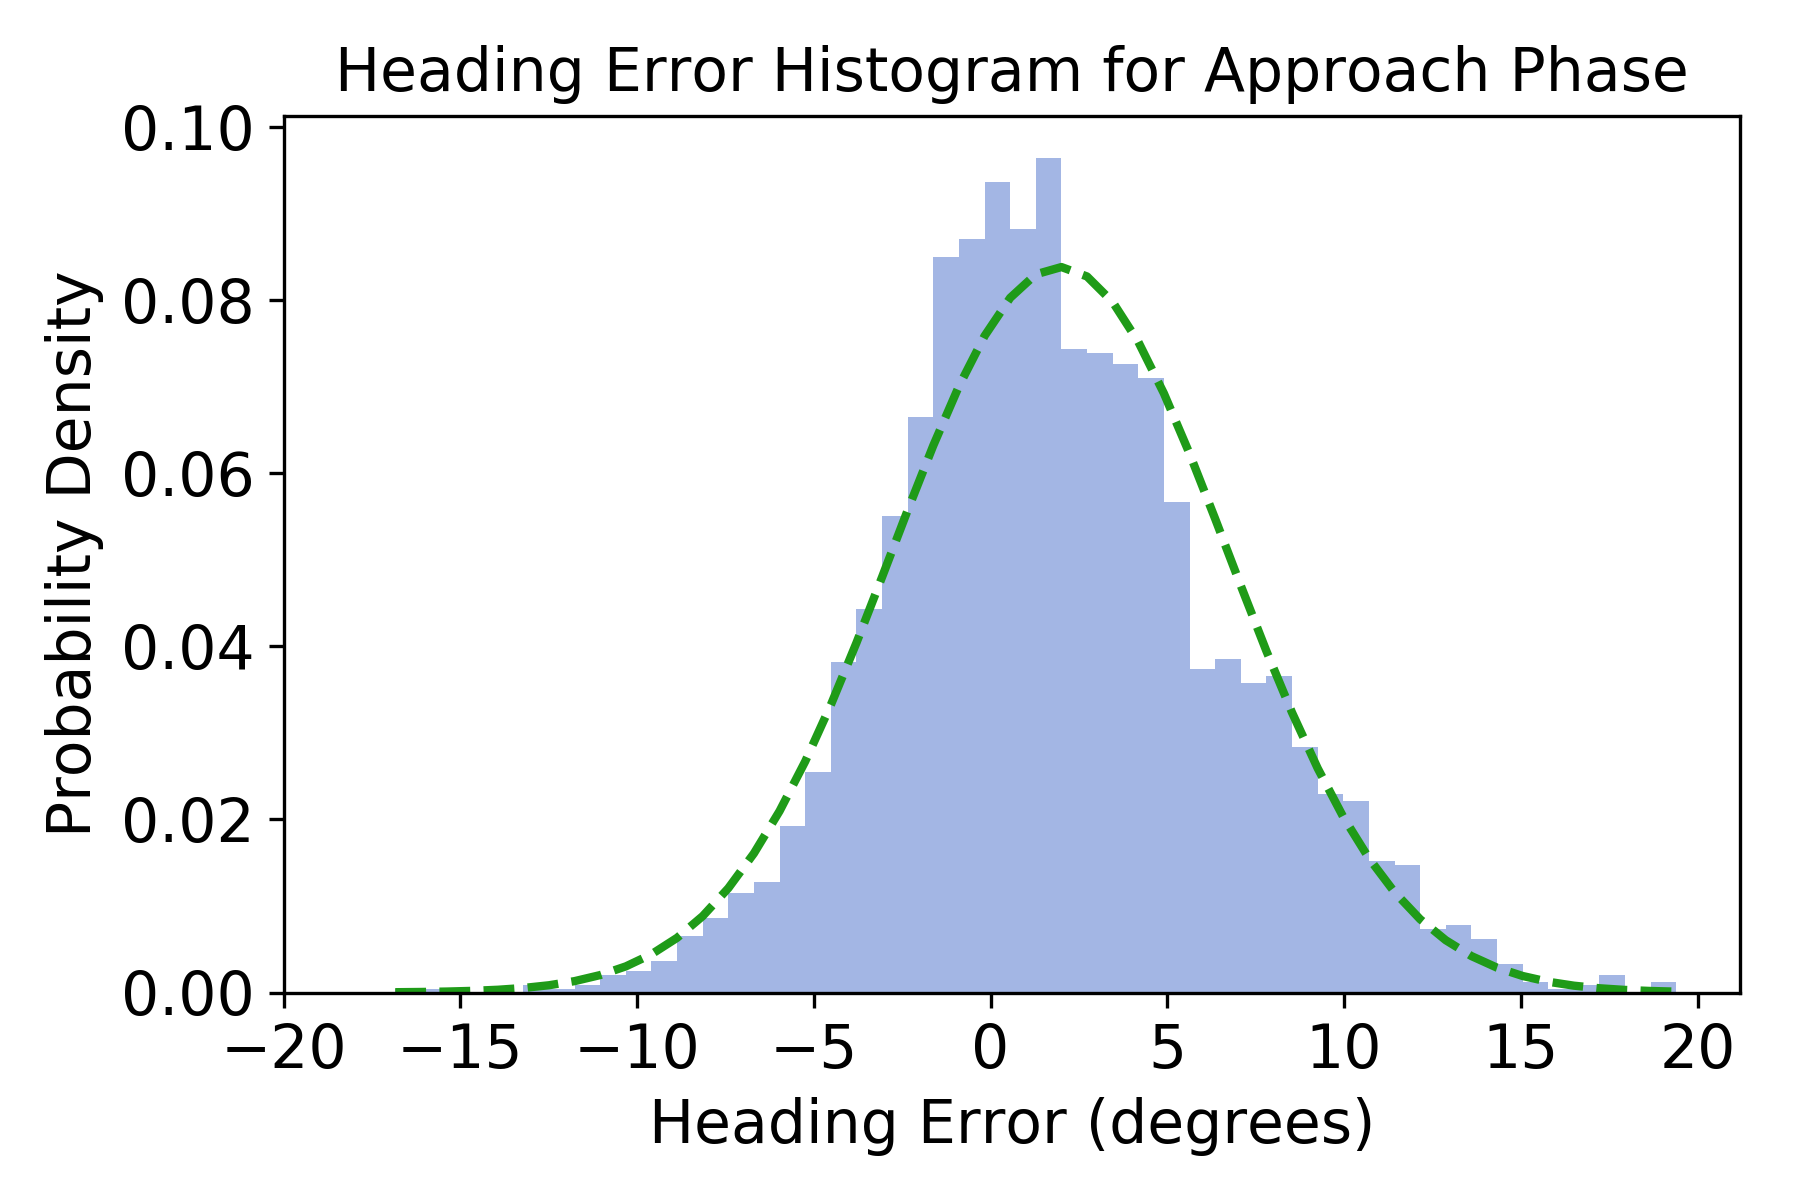
\includegraphics[width=0.45\linewidth]{orig_heading_hist}
        }%
        \caption{Histograms showing the frequencies of values for each parameter during all Approach phases.  Each graph also has a dotted best-fit line to show how close the frequencies adhere to a normal distribution.}
        \label{fig:approach_histograms}
    \end{figure}
    
    
    	%----------
        % FINAL TURN
        %----------
        \subsubsection{Final Turn.}
        
        	Out of the 380 detected approaches; 262 (68.95\%) had a Final Turn subphase, 76 (20.00\%) performed a straight-in approach, and 42 (11.05\%) were not able to detect the runway and, therefore, could not detect whether a Final Turn was performed.  \Cref{fig:final_turn_results_ratios} depicts these ratios.  As mentioned earlier, the 42 \textit{null} runways will be drastically reduced in the future once additional airports and runways are added to the geological database.  Once the airport and runway databases are more complete, the runway error rate should become much more acceptable.
            
            \Cref{fig:final_turn_results_by_risk} gives a comparison of the number of occurrences for each turn error type and Risk Level classification.  This graph is displaying the subset of 262 detected Final Turn subphases found in \Cref{fig:final_turn_results_ratios}.  The figure shows that 76.34\% of the Final Turns resulted in an undershoot and a large proportion (45.420\%) resulted in a Risk Level 2 undershoot.  Those statistics are definitely interesting and are an example of an anomaly that is worth looking into by an aviation expert.  One explanation could be that there is frequently a strong wind component against the aircraft, which could cause the numerous undershoots.  Further analysis such as this could be performed as a future work since wind and other meteorological factors were not taken into consideration in the analyses within this research.
            
            \begin{figure}
            	\centering
                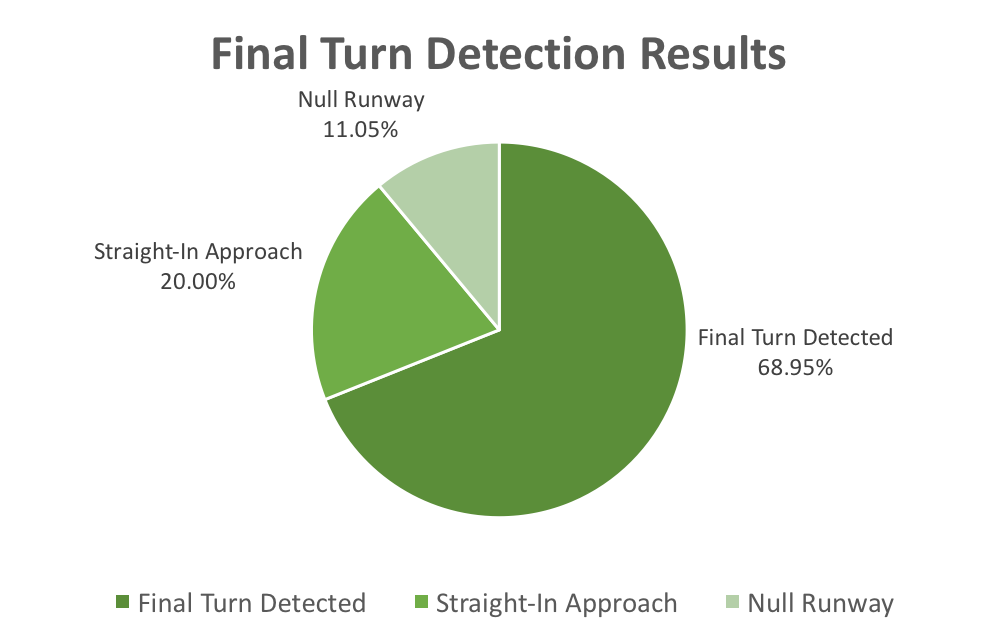
\includegraphics[width=0.75\linewidth]{final_turn_detection_results}
                \caption{Pie chart showing the results from the Final Turn detection algorithm.}
                \label{fig:final_turn_results_ratios}
            \end{figure}
            
            \begin{figure}
            	\centering
                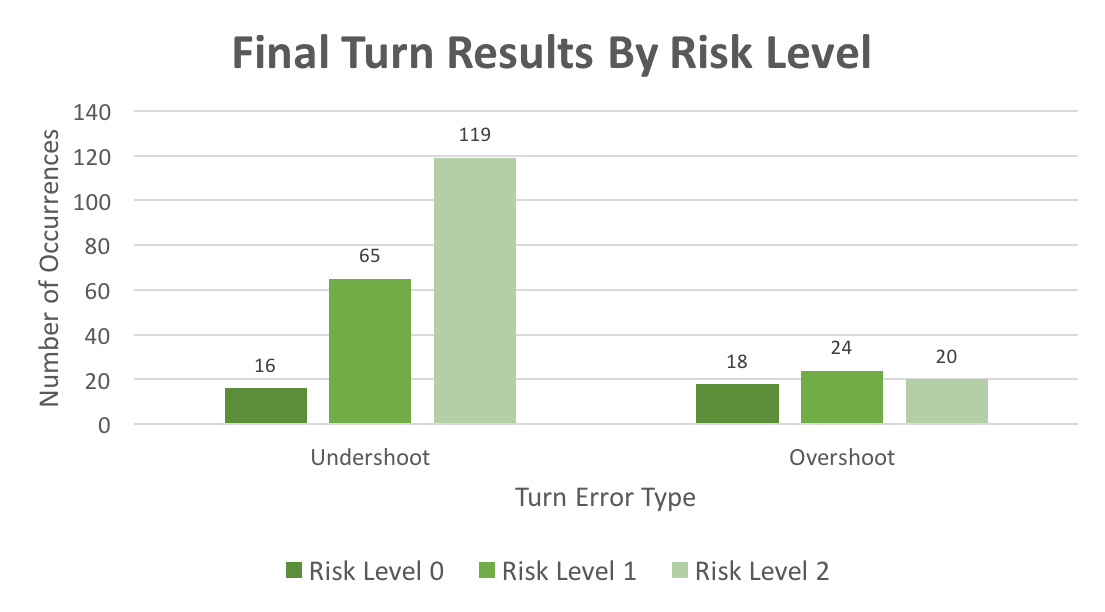
\includegraphics[width=0.95\linewidth]{final_turn_results_by_risk}
                \caption{Frequency of the occurrences of each turn error type for Risk Levels 0, 1, and 2.}
                \label{fig:final_turn_results_by_risk}
            \end{figure}
            
        
        %----------
        % SELF-DEFINED GLIDE PATH
        %----------
%         \subsubsection{Self-defined glide path.}
        
%         	\note{Not sure.  May remove this section since the Web Interface shows exactly the charts that can be created.}


%----------------------------------------
% GRADING METRICS: DEFINE FROM PARAMETER FREQUENCIES
%----------------------------------------
\section{Grading Metrics:  Define From Parameter Frequencies}

	As mentioned in \Cref{ch:methodology}, the goal for creating the Risk Level metrics is to use statistical results from the Approach quality analysis to determine reasonable values that still adhere to the published stable value ranges.  \Cref{subfig:approach_ias_hist,subfig:approach_vsi_hist,subfig:approach_cross_track_hist,subfig:approach_heading_hist} above contain normalized histograms showing the probability density for the parameter values.  These graphs were analyzed by an aviation statistics expert from UND in order to create a safe range (Risk Level 0), a moderate risk range (Risk Level 1), and a high risk range (Risk Level 2) for each parameter of concern.  These graphs will be re-used in the following Sections, but will have additional information showing the value ranges that were created.  The Risk Level 1 values will be a yellow dotted line, while the Risk Level 2 values will be a red dotted line.


	%----------
    % APPROACH
    %----------
%     \subsection{Approach}
    
    	
    %----------
    % IAS
    %----------
    \subsection{Indicated Airspeed Between 55 and 75 knots}
    
          The indicated airspeed values had a mean of 64.401 knots and a standard deviation of 4.535 knots.  The aviation expert stated that the UND standardization manual~\cite{und_flight_manual} has a strict safe range of 61 -0/+5 knots, and thus anything less than 61 knots should be automatically classified as a Risk Level 2.  He advised the higher Risk Level 1 should begin with any value greater than 66 knots due to the same rule.  Lastly, he advised setting the higher Risk Level 2 at 71 knots in order to use the consistent 5 knots increment, which is also relatively close to one standard deviation.  As is shown in \Cref{fig:revised_ias_hist}, the graph is slightly skewed to the right following the -0/+5 knots rule, which is more lenient towards faster speeds than slower speeds.

		\begin{figure}
			\centering
            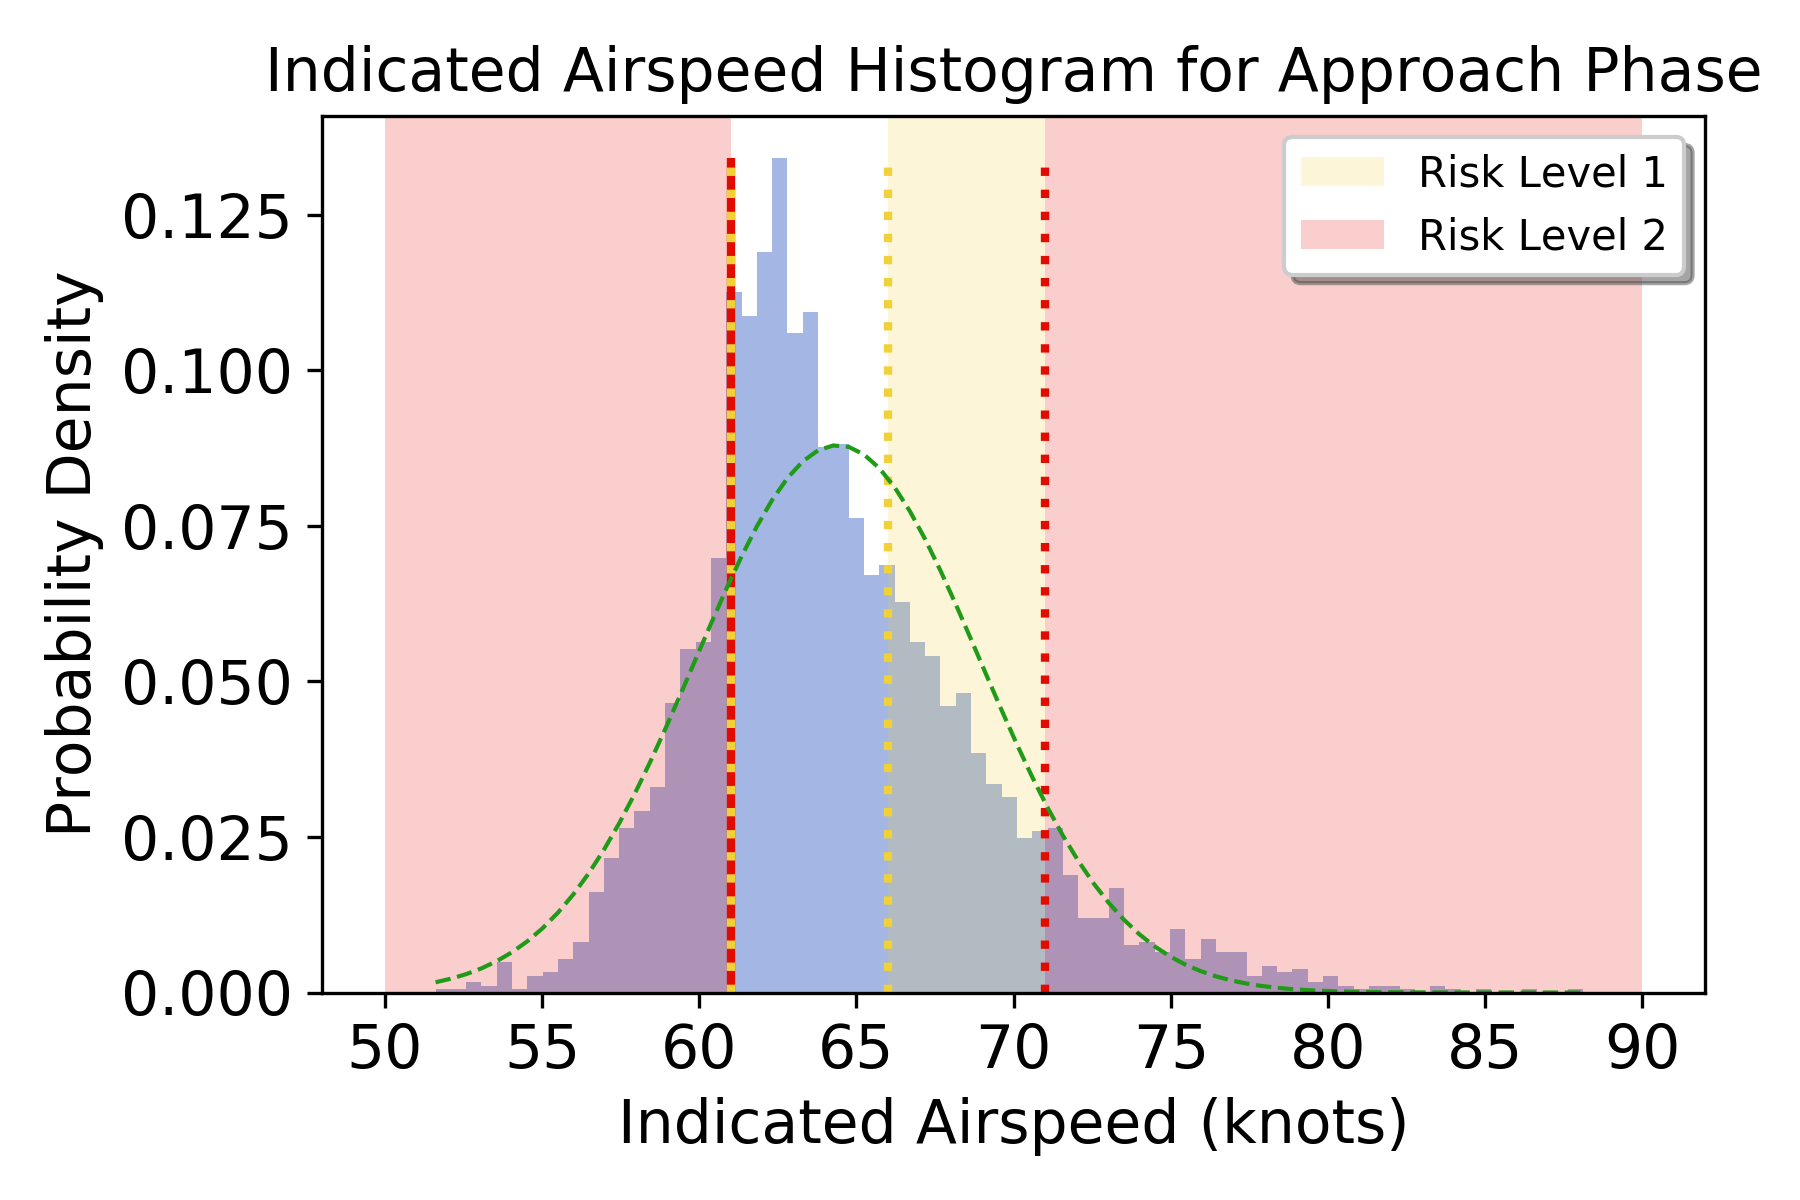
\includegraphics[width=\linewidth]{revised_ias_hist}
            \caption{Histogram for indicated airspeed ($\mu = 64.401, \sigma = 4.535$).  The safe range is between 61 and 66 knots.  There is no lower Risk Level 1 since the Risk Level 2 is anything less than 61 knots.  The higher Risk Level 1 range is between 66 and 71 knots, and the Risk Level 2 is anything greater than 71 knots.}
            \label{fig:revised_ias_hist}
		\end{figure}



    %----------
    % VSI
    %----------
    \subsection{Vertical Speed Indicated Greater Than -1000 ft/min}
    
    	The vertical speed indicated values had a mean of -364.528 ft/min and a standard deviation of 181.210 ft/min.  Although the UND standardization manual states that a vertical speed greater than -1000 ft/min should be achieved for a stabilized approach, the aviation expert stated that a safe range of -800 to -500 ft/min is typically suggested instead of the wide range provided in the manual.  The lower Risk Level 1 is any value that is less than -800 ft/min, and the lower Risk Level 2 is any value less than -1000 ft/min in order to adhere to the stable limit given in the manual.  The higher Risk Level 1 is any value greater than -500 ft/min, and the higher Risk Level 2 is any value greater than -250 ft/min.  These higher limits were chosen because if the aircraft is descending at 250 ft/min, it will typically result in an unsafe and shallow glide slope.  \Cref{fig:revised_vsi_hist} shows these limits and shows that the values are slightly skewed to the left, which corresponds to the risk limits that we've set.

		\begin{figure}
			\centering
            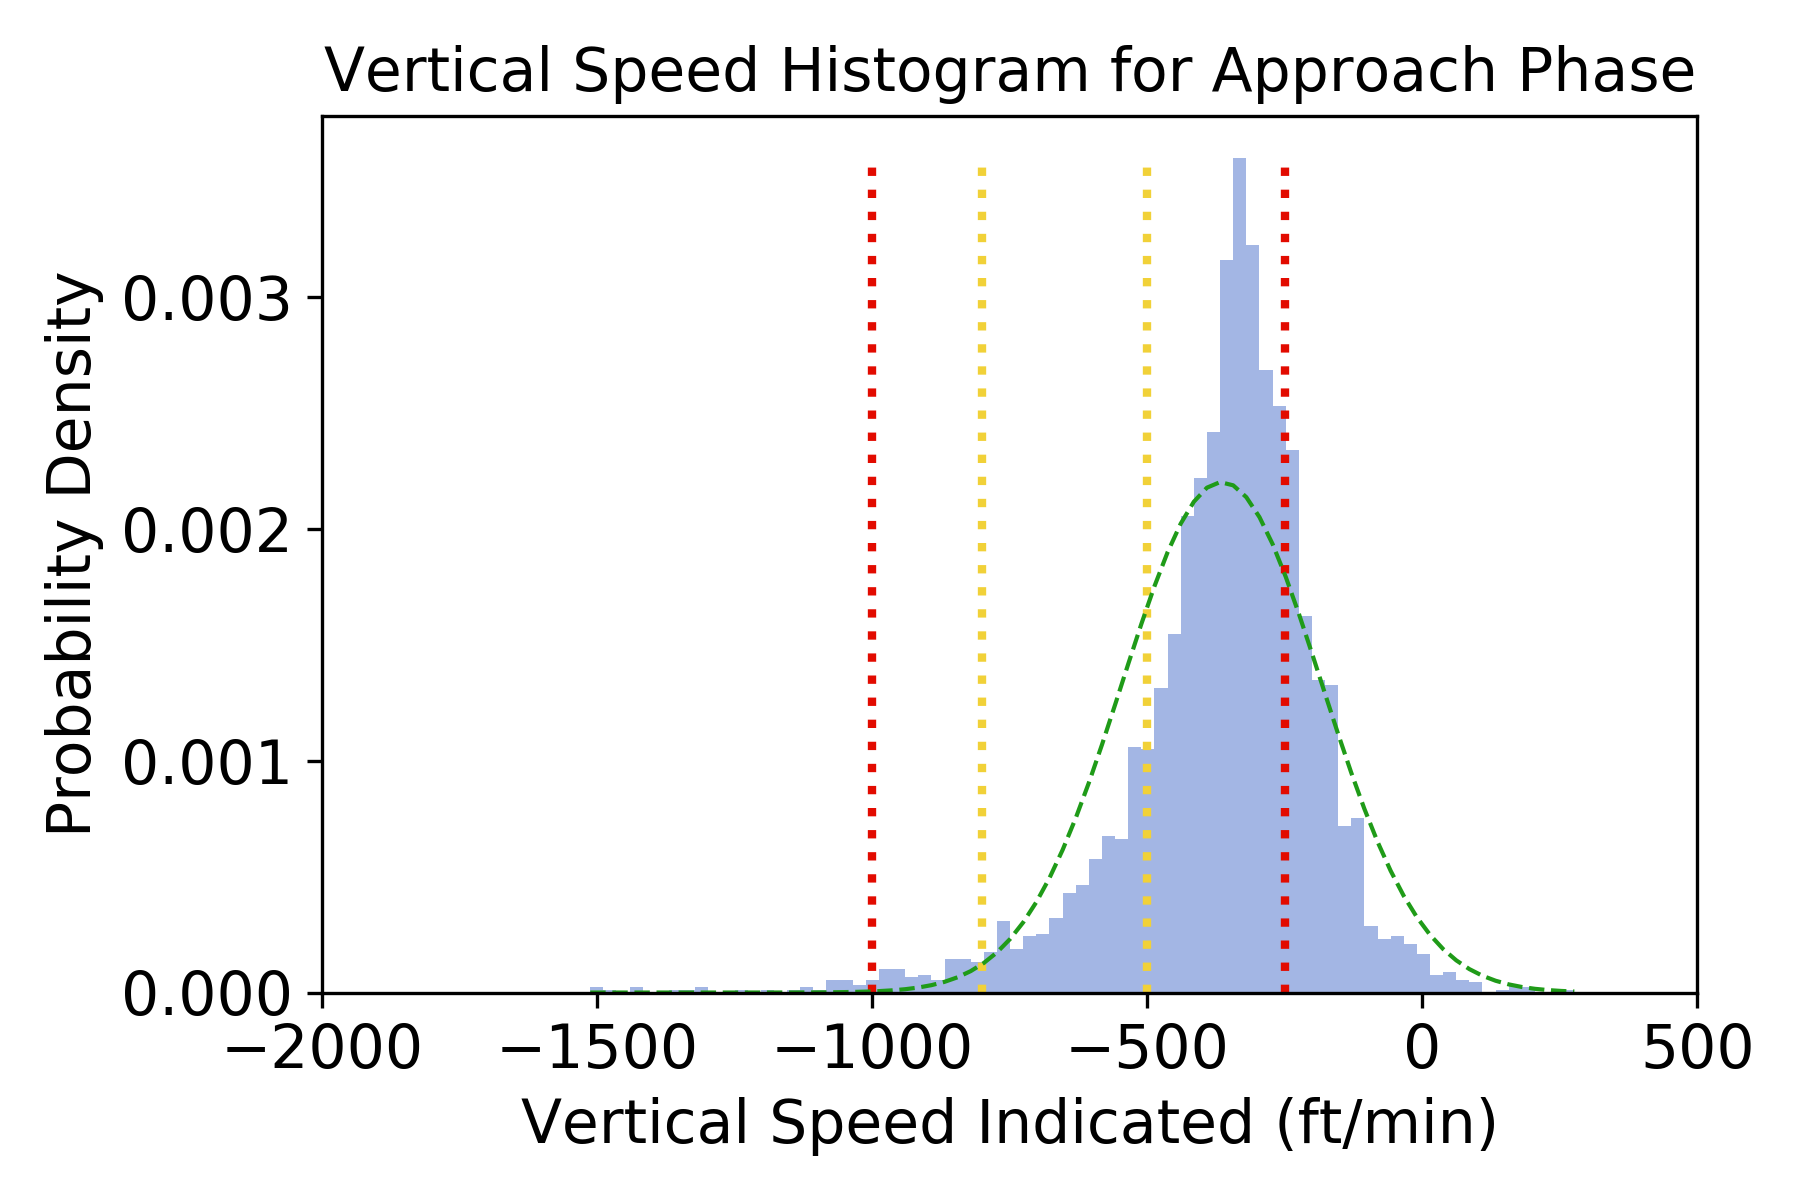
\includegraphics[width=\linewidth]{revised_vsi_hist}
            \caption{Histogram for vertical speed indicated ($\mu = -364.528, \sigma = 181.210$).  The safe range is between -800 and -500 ft/min.  The lower Risk Level 1 range is between -1000 and -800 ft/min, and the Risk Level 2 is anything less than -1000 ft/min.  The higher Risk Level 1 range is between -500 and -250 ft/min, and the Risk Level 2 is anything greater than -250 ft/min.}
            \label{fig:revised_vsi_hist}
		\end{figure}



    %----------
    % CROSS TRACK ERROR
    %----------
    \subsection{Absolute Cross Track Error Less Than 50 ft}
    
    	The cross track error values had a mean of -4.542 feet and a standard deviation of 15.499 feet.  \Cref{fig:revised_cross_track_hist} displays the histogram for these values and it can be seen that the graph is relatively normal with a slight skew to the left.  The aviation expert stated that a deviation in cross track error is not as risky as a deviation in airspeed or vertical speed.  Thus, a wider safe range was defined as -40 feet to 40 feet, which is about where the tails wane on both sides.  Consequently, the lower and higher Risk Level 1 ranges are -50 feet to -40 feet and 40 feet to 50 feet, respectively.  The lower and higher Risk Level 2 values are then -50 feet and 50 feet, respectively, in order to correspond with the original stable limits that were used.
        
		\begin{figure}
			\centering
            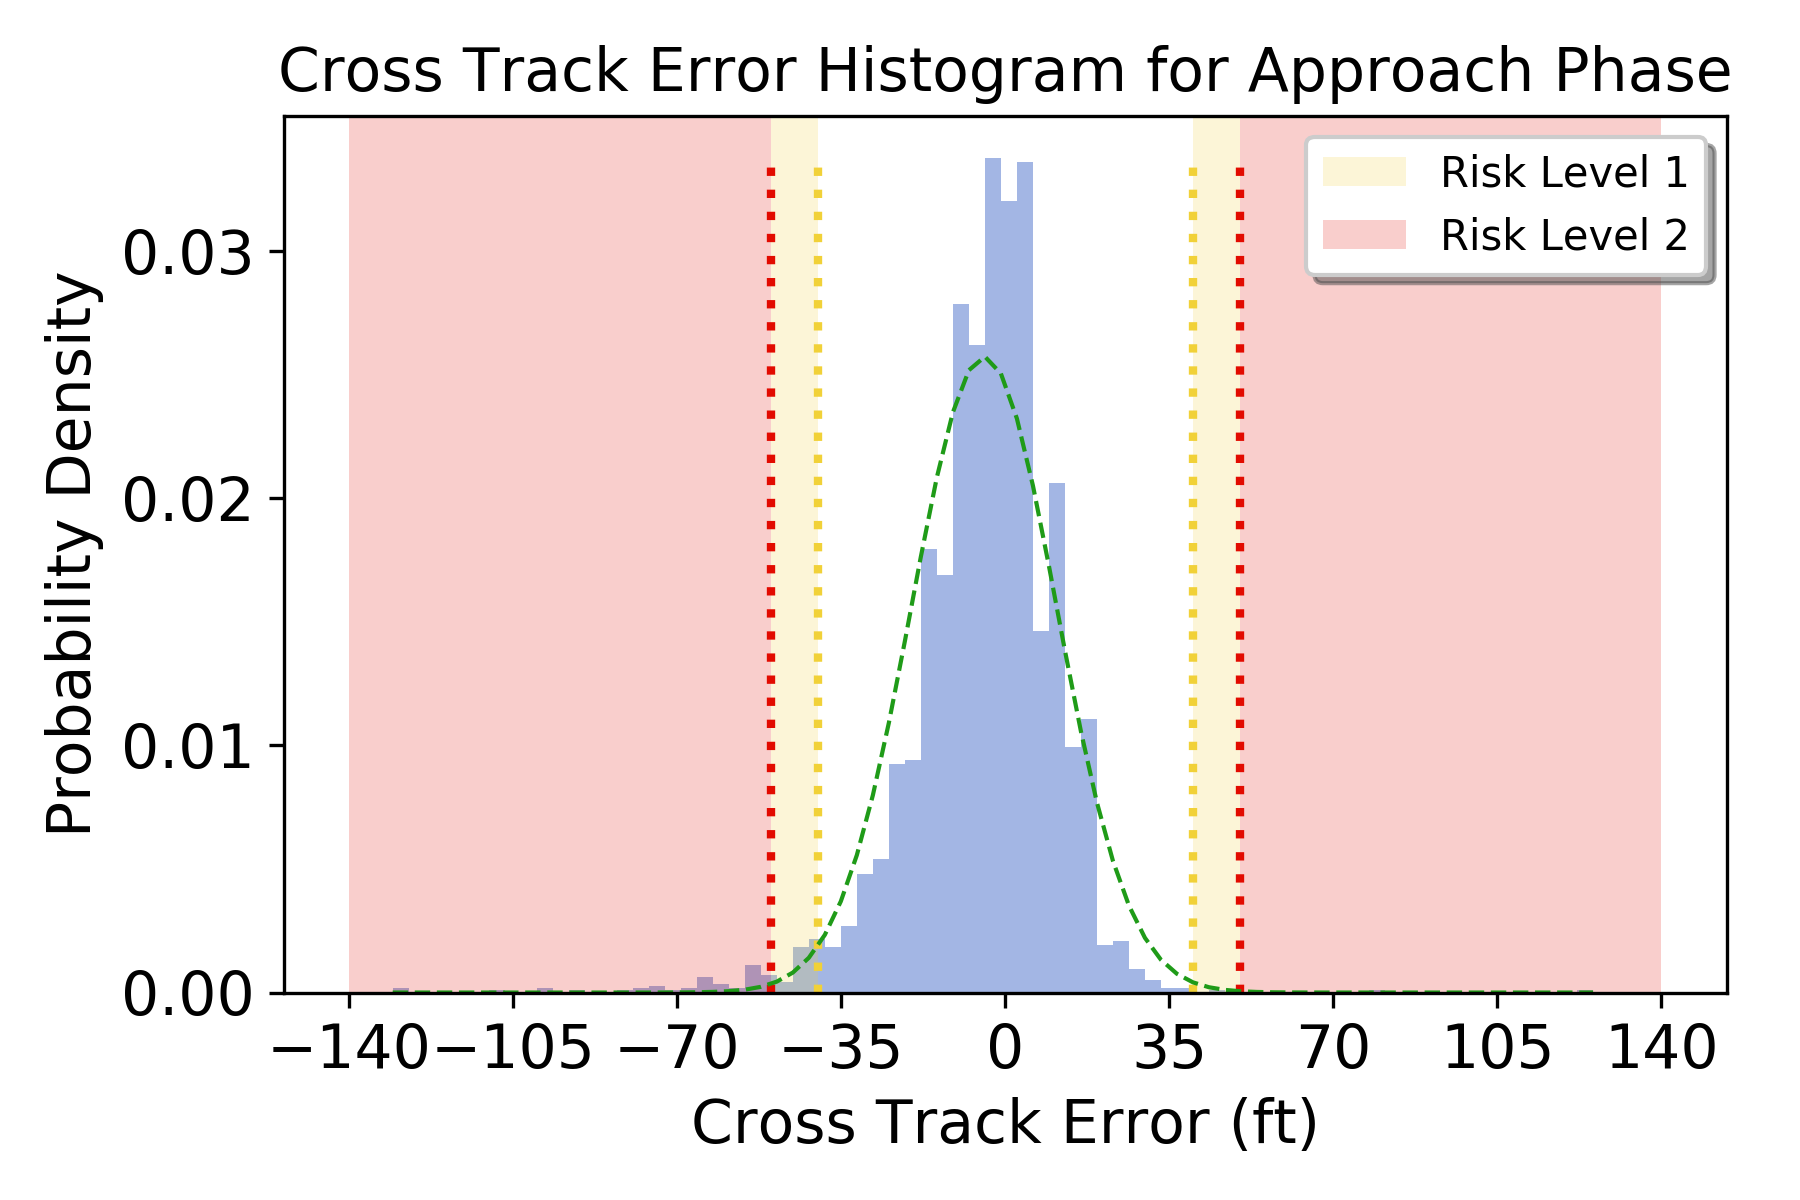
\includegraphics[width=\linewidth]{revised_cross_track_hist}
            \caption{Histogram for cross track error ($\mu = -4.542, \sigma = 15.499$).  The safe range is between -40 and 40 ft.  The lower Risk Level 1 range is between -50 and -40 ft, and the Risk Level 2 is anything less than -50 ft.  The higher Risk Level 1 range is between 40 and 50 ft, and the Risk Level 2 is anything greater than 50 ft.}
            \label{fig:revised_cross_track_hist}
		\end{figure}



    %----------
    % HEADING ERROR
    %----------
    \subsection{Absolute Heading Error Less Than 10 degrees}
    
    	The heading error values had a mean of $1.958^\circ$ and a standard deviation of $4.761^\circ$.  Similar to cross track error, the aviation expert stated that heading error is not as risky as error in the other parameters.  He also mentioned that heading error is slightly more difficult to judge without knowing the wind component on the aircraft since the pilot may have to purposely direct the aircraft several degrees off-center in order to counteract the push of the wind.  Both of these facts means that the safe range for heading error will contain a majority of values.  With that said, the expert advised using a safe range of $-15^\circ$ to $15^\circ$.  The lower and higher Risk Level 1 ranges are from $-20^\circ$ to $-15^\circ$ and $15^\circ$ to $20^\circ$, respectively.  Consequently, the lower and higher Risk Level 2 values are $-20^\circ$ and $20^\circ$, respectively.  The histogram for heading error, as shown in \Cref{fig:revised_heading_hist}, appears to best fit a normal distribution.
        
        \begin{figure}
			\centering
            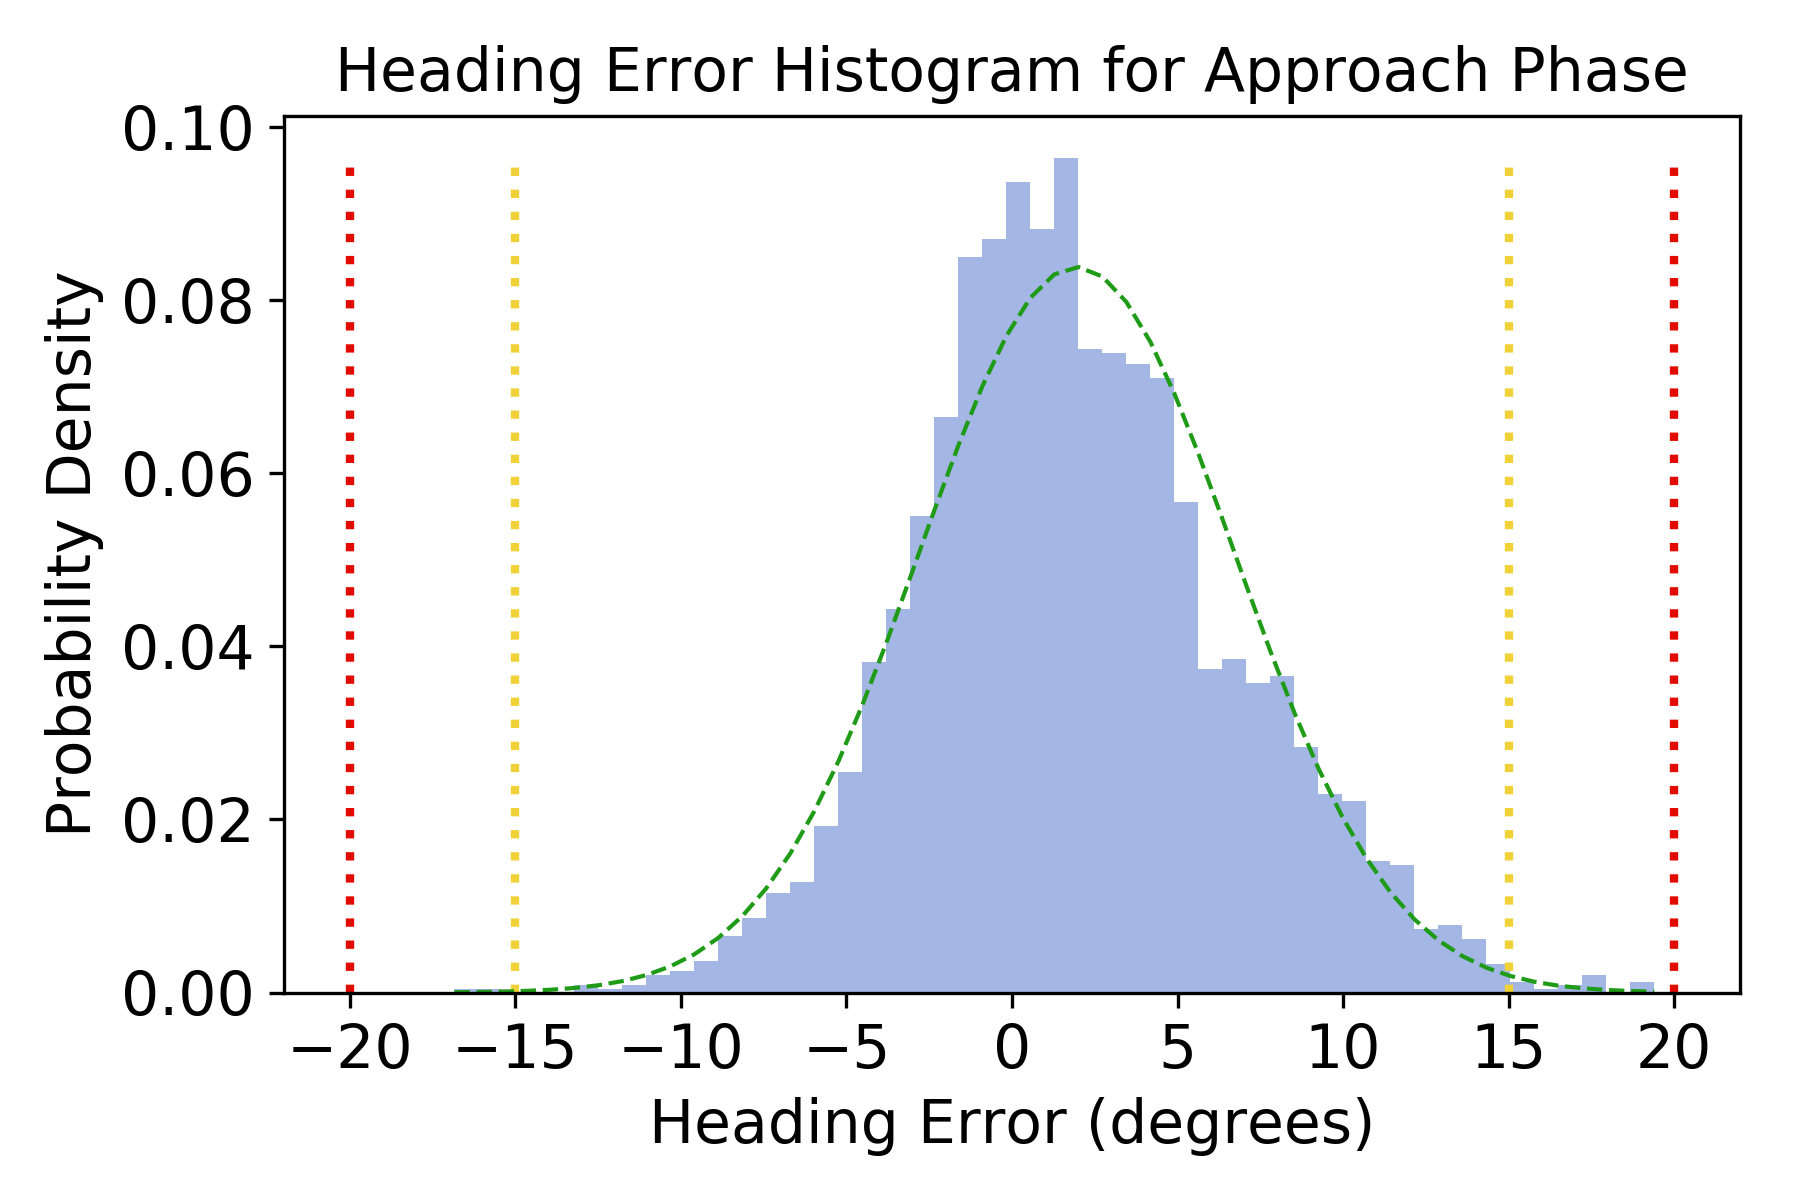
\includegraphics[width=\linewidth]{revised_heading_hist}
            \caption{Histogram for heading error ($\mu = 1.958, \sigma = 4.761$).  The safe range is between -15 and 15 degrees.  The lower Risk Level 1 range is between -20 and -15 degrees, and the Risk Level 2 is anything less than -20 degrees.  The higher Risk Level 1 is between 15 and 20 degrees, and the Risk Level 2 is anything greater than 20 degrees.}
            \label{fig:revised_heading_hist}
		\end{figure}
        
        
        
        \begin{table}
        	\centering
            \caption{\small{blah}} \label{tab:metrics_values}
            \vspace{3pt}
            \begin{tabular}{@{} l l | l l @{}}
            \hline\noalign{\smallskip}
            \multicolumn{2}{c|}{\bfseries Event} & \bfseries Risk Level 1 & \bfseries Risk Level 2 \\
            \noalign{\smallskip}
            \hline
            \noalign{\smallskip}
            
            \multirow{2}{*}{Indicated Airspeed} & low  & N.A.     & 61 knots \\
                                                & high & 66 knots & 71 knots \\ 
			\midrule
            \multirow{2}{*}{Vertical speed} & low  & -800 ft/min & -1000 ft/min \\
                                            & high & -500 ft/min & -250 ft/min \\
            \midrule
            \multirow{2}{*}{Cross track error} & low  & -40 ft & -50 ft \\
                                               & high & 40 ft  & 50 ft \\
            \midrule
            \multirow{2}{*}{Heading error} & low  & $-15^\circ$ & $-20^\circ$ \\
                                           & high & $15^\circ$  & $20^\circ$ \\
            \midrule
            \end{tabular}
        \end{table}
            

%----------------------------------------
% GRADING METRICS: RESULTS
%----------------------------------------
\section{Grading Metrics:  Experiment Results}

	\note{Results found from using metrics on analysis results.}
    
    
%----------------------------------------
% WEB INTERFACE
%----------------------------------------
\section{Web Interface}

	This Section details the newly developed web pages for the NGAFID, which dynamically display results based on the user's chosen filters.  At the time of this writing, there have been new tools developed for the Approach, Final Turn, and self-defined glide path analyses.  Each tool will be discussed further in the subsequent Subsections.
    
    
    %----------
    % APPROACH
    %----------
    \subsection{Approach}
    
    	A new web page was implemented in the NGAFID for the purpose of dynamically displaying the Approach analysis results produced by the \toolname\ to users (\Cref{fig:approach_tool_screenshot}).  The results are given in four tabs, one for each parameter, as histograms over a specified date range.  A user is able to dynamically add additional date ranges, which will create an additional series in the chart for comparison.  This feature can be used to detect changes in trends over time.  A user is also, optionally, able to filter the results to an airport and further filter to a single runway.  This will allow users to identify trends that are potentially occurring at a specific runway but not at any other runways.
    
    	\begin{figure}
    		\centering
            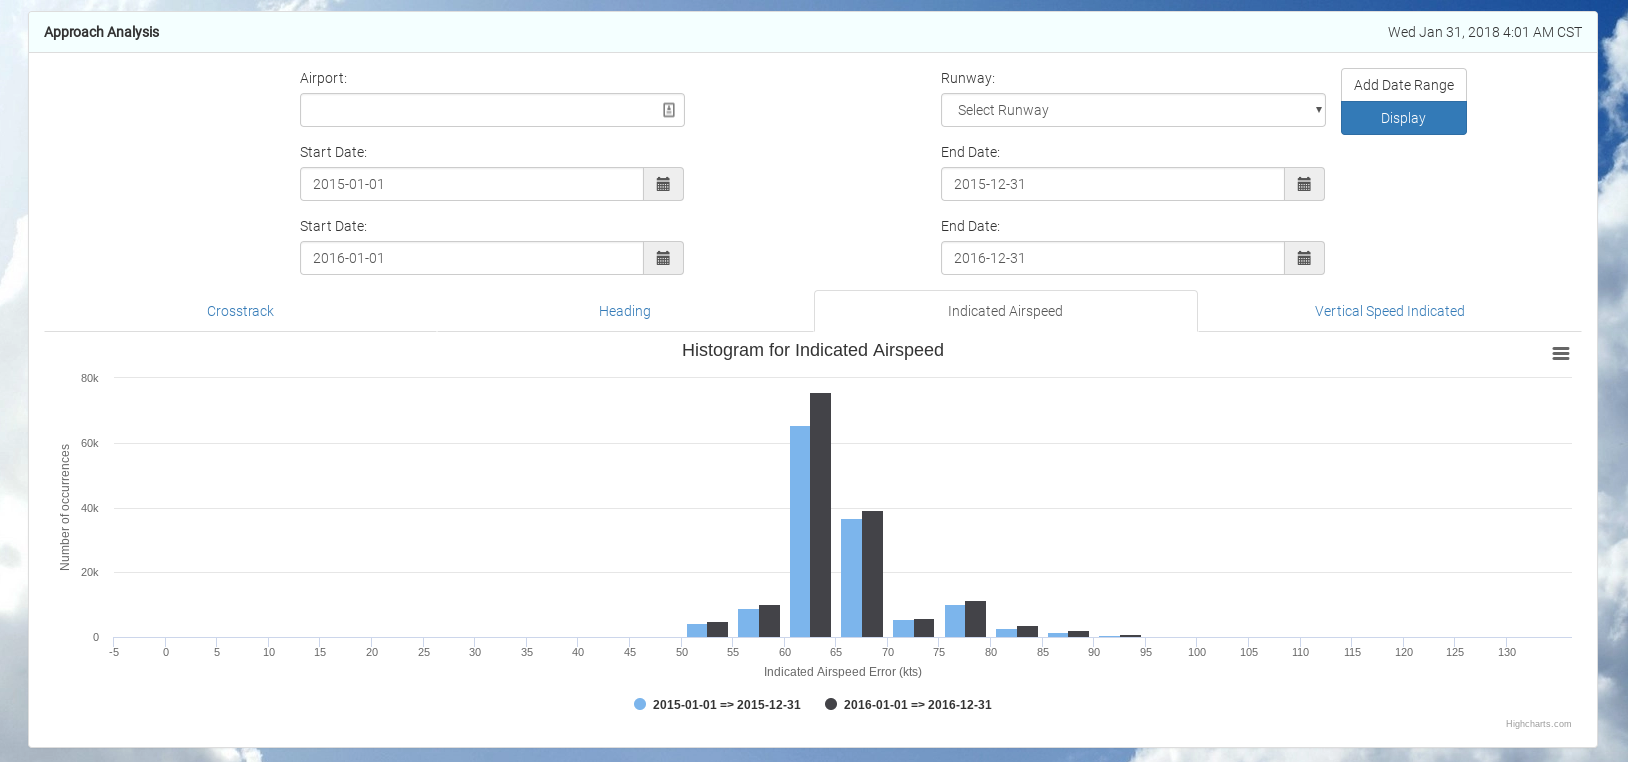
\includegraphics[width=\linewidth]{img/approach_tool_screenshot}
            \caption{A screenshot of the Approach analysis tool on the NGAFID.  It is showing the histogram for indicated airspeed error with two date range filters: 2015-01-01 to 2015-12-31 and 2016-01-01 to 2016-12-31.  The frequency of exceedances can be seen with all values that fall outside of the 55-75 knots range.}
            \label{fig:approach_tool_screenshot}
    	\end{figure}
    
    
    %----------
    % FINAL TURN
    %----------
    \subsection{Final Turn}
    
    	The tool developed for analyzing Final Turn phases in the NGAFID was implemented with two modes:  \textit{(i)} ``Single Flight'' and \textit{(ii)} ``Aggregate''.
    
    	For the ``Single Flight'' mode, the user can input an ID for a specific flight they'd like to analyze (\Cref{fig:single_ttf_screenshot}).  Once the user clicks the ``Display Single Flight'' button, the interactive map then dynamically transitions to the first approach for that flight.  The map will only display one approach at a time; although, there are tabs across the top for each approach which the user can choose.  Once a different tab is chosen, the map automatically transitions the view to that corresponding approach.  The flight path shows different color codings for the separate Final Turn, Approach, and Landing phases as well as different colors for the Final Turn specifically depending on the severity of the turn error.  A Level 1 turn error will be colored yellow, while a Level 2 turn error will be colored red.  If the turn error is less than the Level 1 criteria, it is colored green.  The user is also able to download a PNG screenshot of the map by clicking the ``Download PNG'' button.
        
        For the ``Aggregate'' mode; the user can choose a specific airport, runway, and month and year combination; which will then display all the approaches that occurred at the chosen runway during the chosen time-frame (\Cref{fig:agg_ttf_screenshot}).  This mode allows a user to see trends in Final Turn phases during a given time span.  This mode displays the same color code scheme as the ``Single Flight'' mode.
    
    	\begin{figure}
    		\centering
            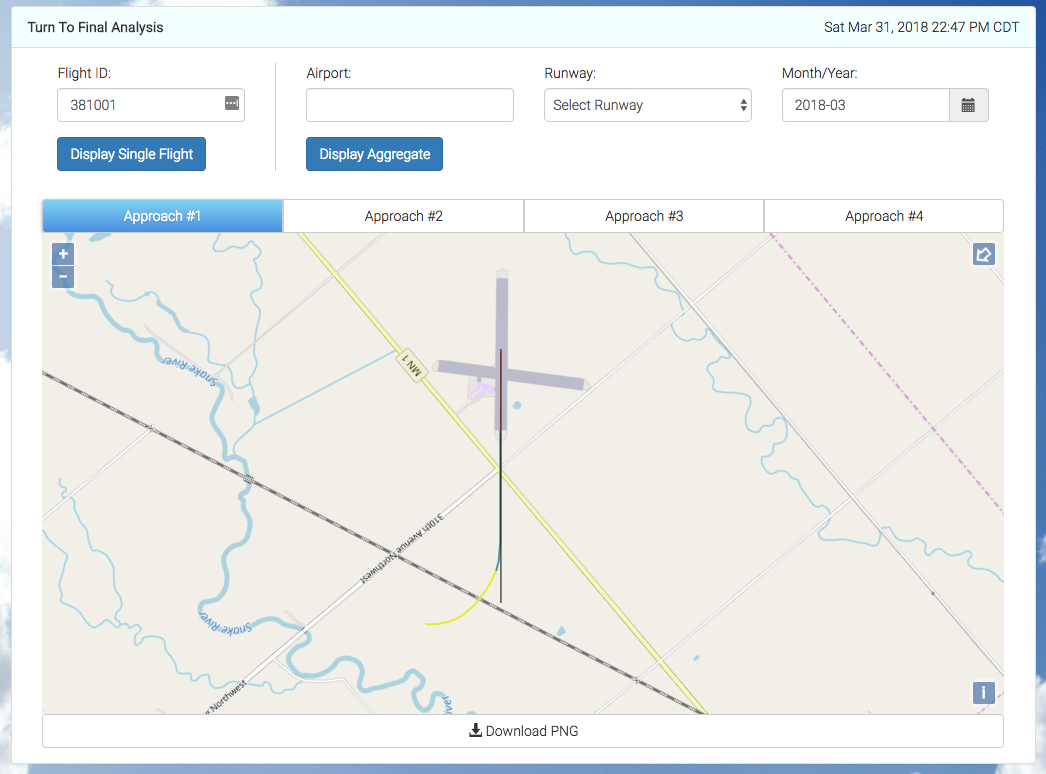
\includegraphics[width=\linewidth]{img/single_ttf_screenshot}
            \caption{A screenshot of the Final Turn analysis tool on the NGAFID in ``Single Flight'' mode.  It is currently showing Approach \#1 for Flight ID \#381001.  Approach \#1 shown here had a Level 1 (yellow color code) undershoot.}
            \label{fig:single_ttf_screenshot}
    	\end{figure}
        
        \begin{figure}
    		\centering
            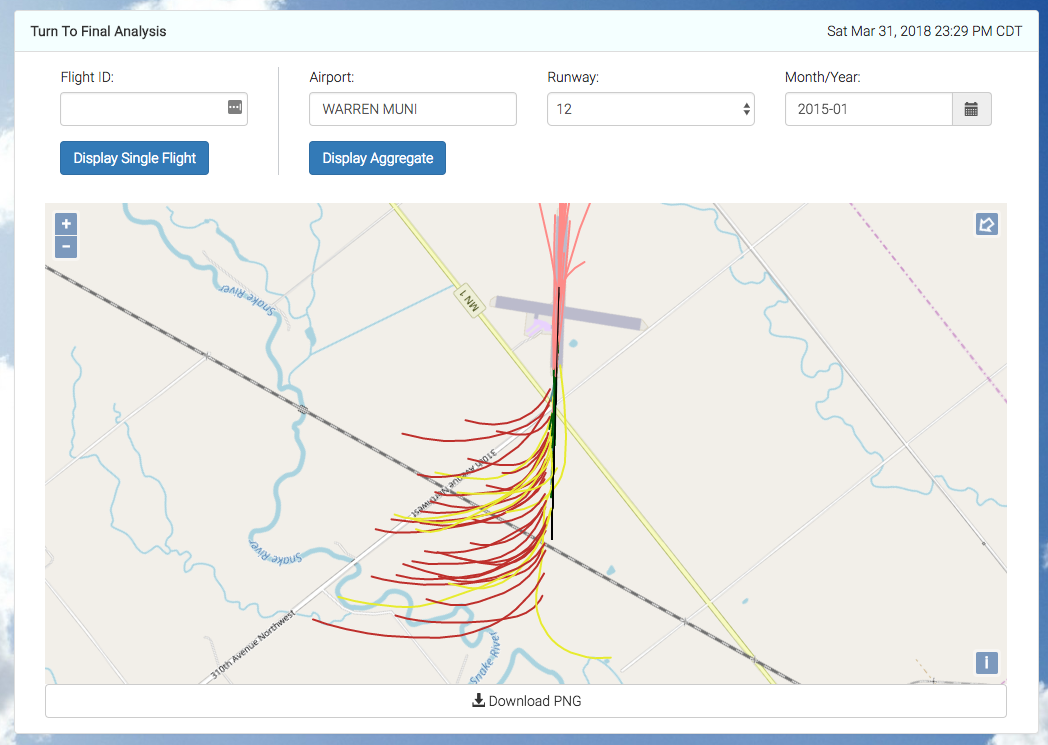
\includegraphics[width=\linewidth]{img/agg_ttf_screenshot}
            \caption{A screenshot of the Final Turn analysis tool on the NGAFID in ``Aggregate'' mode.  It is currently showing all approaches at the Warren Municipal Airport (KD37) for Runway 12 during the month of January 2015.  The many red and yellow lines coming in from the left side mean that a majority of the turns were Level 1 \& 2 undershoots.}
            \label{fig:agg_ttf_screenshot}
    	\end{figure}
    
    %----------
    % SELF-DEFINED
    %----------
    \subsection{Self-Defined Glide Path}
    
    	The tool implemented in the NGAFID for displaying the results of the self-defined glide path analysis currently only supports an aggregate mode (\Cref{fig:self_defined_screenshot}).  It works similarly to the Final Turn tool as the user chooses an airport, runway, and month and year combination.  This will then display a sideways histogram of all the approaches at the given runway during the given time-frame.  The y-axis shows glide path angles from $0^\circ$ to $10^\circ$ in $5^\circ$ increments, and the x-axis shows the number of occurrences that fell within each angle bin.  Lastly, the user can download an image of the displayed chart by clicking the ``hamburger'' menu button.
    
    	\begin{figure}
    		\centering
            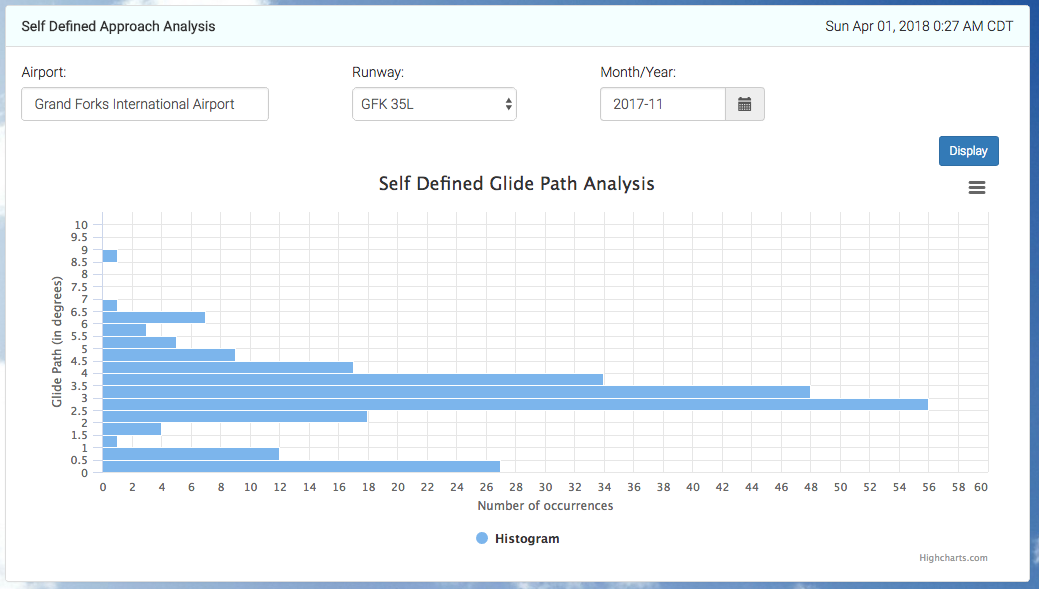
\includegraphics[width=\linewidth]{img/self_defined_screenshot}
            \caption{A screenshot of the Self-Defined Approach analysis tool on the NGAFID.  It is currently showing all approaches at the Grand Forks International Airport (KGFK) for Runway 35L during the month of November 2017.  It displays a sideways histogram with glide path angles on the y-axis and the number of occurrences for each angle on the x-axis.}
            \label{fig:self_defined_screenshot}
    	\end{figure}


%----------------------------------------
% PERFORMANCE
%----------------------------------------
\section{Performance}

	A secondary aspect of this research is to minimize the execution time so  the analysis only adds a minimal amount of time to a flight being imported into the NGAFID system.  The results of the benchmarking tests showed that the linearly executing application ran for an average of XXX.XXX seconds over the 100 randomly tested flights.  On the other hand, the parallel application ran for an average of XX.XXX seconds over the same flights.  This means the average per-flight execution times for the linear and parallel applications were X.XXX and X.XXX seconds, respectively.  As a result, the parallelized application had a XX.XXX\% speedup, which is fairly significant.  %A summary of the benchmarking tests and other relevant statistics are given in \Cref{tab:performance_results}.
    \note{Fill in timing results.}
    
    As further evidence, the parallel application was tested on a larger subset of flights to see if the average execution time remained stable, in which it was tested on 5,272 flights.  For this test, the parallel application was able to analyze the data and insert all the results into the database in XXXX.XXX seconds.  This gives a per-flight execution time of X.XXX seconds, which is slightly less than the average for 100 flights.  The reasoning behind this can most likely be attributed to the fact that spinning up the sub-processes creates a substantial overhead.  Thus, the longer the application is able to execute, the greater performance gain will be received.  This will, of course, start to show diminishing returns as with any other parallel computing application.
    
    
    \begin{table}[tb]
    	\centering
        \caption{\small{Performance of Linear v. Parallel Execution Times}} \label{tab:performance_results}
        \vspace{3pt}
        \begin{tabular}{@{} >{\centering\arraybackslash} m{.23\linewidth} S[table-format=3.3] S[table-format=2.3] @{}}
            \hline\noalign{\smallskip}
            \bfseries Run & \bfseries Linear (sec) & \bfseries Parallel (sec) \\
            \noalign{\smallskip}
            \hline
            \noalign{\smallskip}
             1 & 591.935 & 57.295 \\ \hline
             2 & 576.774 & 60.282 \\ \hline
             3 & 586.009 & 57.830 \\ \hline
             4 & 597.643 & 62.489 \\ \hline
             5 & 591.170 & 57.578 \\ \hline
             6 & 585.834 & 62.702 \\ \hline
             7 & 593.711 & 65.064 \\ \hline
             8 & 587.177 & 66.167 \\ \hline
             9 & 586.059 & 58.108 \\ \hline
            10 & 590.012 & 56.501 \\ \hline
            \hline
            \bfseries Average           & 588.632 & 60.402   \\ \hline
            \bfseries Latency / flight  &   5.886 &  0.604   \\ \hline
            \bfseries Speedup           &         & 90.255\% \\ \hline
        \end{tabular}
    \end{table}
    
    
    
    
\chapter{Conclusion} \label{ch:conclusion}




%----------------------------------------------------------------------------------------
%	THESIS CONTENT - APPENDICES
%----------------------------------------------------------------------------------------

\appendix

% Include the appendices of the thesis as separate files from the Appendices folder
% Uncomment the lines as you write the Appendices

% \chapter{Appendix Title Here} % Main appendix title
\label{app:appendix_a} % For referencing this appendix elsewhere, use \ref{AppendixA}

Write your Appendix content here.

%\input{Appendices/AppendixB}
%\input{Appendices/AppendixC}

\backmatter{}

%----------------------------------------------------------------------------------------
%	REFERENCES
%----------------------------------------------------------------------------------------

\bibliographystyle{IEEEtran}
\bibliography{bibliography}

\end{document}

